% ThinkAlgo — Đếm và Xác suất — Lớp 7
% Edition: teacher (with solutions), VI.  Generated by build_grade7.py — edit body/ and rebuild.
\documentclass[11pt]{article}
\newif\ifsol \soltrue
\usepackage{iftex}
\ifPDFTeX
  \usepackage[utf8]{inputenc}\usepackage[T5]{fontenc}
\else
  \usepackage{fontspec}
\fi
\usepackage[a4paper,top=2.95cm,headheight=1.5cm,headsep=0.45cm,bottom=3.1cm,left=1.9cm,right=1.9cm]{geometry}
\usepackage{amsmath,amssymb}
\usepackage{tikz}\usetikzlibrary{calc,shadows,shapes.geometric}
\usepackage[most]{tcolorbox}
\usepackage{enumitem}
\usepackage{array}
\usepackage{tabularx}
\usepackage{colortbl}
\usepackage{comment}
\usepackage{needspace}
\usepackage{fancyhdr}
\usepackage{fontawesome5}
\usepackage{graphicx}
\usepackage{microtype}
% PDF outline (bookmarks) so each chapter shows in the reader's outline — does not change the page layout
\usepackage[hidelinks,unicode,bookmarksnumbered=false,bookmarksopen=true,bookmarksopenlevel=0]{hyperref}
\usepackage{bookmark}
\usetikzlibrary{decorations.pathreplacing,arrows.meta,angles,quotes,patterns,positioning,through,intersections}

% ---------------- palette: navy family + subtle light tint; orange ONLY in the logo ----------------
% ----- EXACT palette from the user's original main (36).tex (vivid, not pale) -----
\definecolor{tmBlue}{RGB}{66,133,244}   % problem / header / section
\definecolor{tmGreen}{RGB}{52,168,83}   % solution
\definecolor{tmOrange}{RGB}{255,152,0}  % example
\colorlet{Navy}{tmBlue}                 % header rule / section heading / badge / divider
\definecolor{NavyD}{HTML}{222222}       % solution body text (dark, readable)
\colorlet{Gold}{Navy}
\colorlet{ProbBlue}{tmBlue}             % problem boxes
\colorlet{SolGreen}{tmGreen}            % solution boxes
\definecolor{AnsRed}{HTML}{E02424}      % vivid red for answers / totals
\definecolor{CardGreen}{HTML}{34A853}   % digit-card green
\definecolor{StarGold}{HTML}{F2B134}    % difficulty star (gold)
\definecolor{KidOrange}{HTML}{DE8A2C}   % logo accent only
\definecolor{Ink}{HTML}{1F2733}       % body text
\definecolor{Slate}{HTML}{5B6A82}     % muted labels
\definecolor{Line}{HTML}{C6D0DF}      % light hairlines / student boxes
\definecolor{Tint}{HTML}{EDF1F7}      % pale panel fill (worked solution / answer)
% aliases so older names keep working
\colorlet{TextDark}{Ink}\colorlet{TextGray}{Slate}\colorlet{Soft}{Slate}
\colorlet{CardLine}{Line}\colorlet{Teal}{Navy}\colorlet{ProbB}{Navy}\colorlet{SolG}{Navy}
% bright, kid-friendly colours for bar-model (sơ đồ đoạn thẳng) blocks
\definecolor{tmPurple}{RGB}{124,77,226}
\definecolor{tmTeal}{RGB}{0,150,136}
\definecolor{tmPink}{RGB}{233,30,99}
\AtBeginDocument{\color{Ink}}
\raggedbottom  % natural flow, even spacing (no stretched gaps)
\setlength{\parindent}{0pt}\setlength{\parskip}{0.18em}
\renewcommand{\arraystretch}{1.35}
\providecommand{\AnsWord}{Đáp số}

% ---------------- brand logo (original mark) ----------------
\newcommand{\logomark}[1]{\begin{tikzpicture}[baseline=-0.55ex,scale=#1]
  \draw[KidOrange,line width=1.5pt] (-0.27,0) .. controls (-0.27,0.23) and (0,0.23) .. (0,0)
        .. controls (0,-0.23) and (-0.27,-0.23) .. (-0.27,0);
  \draw[Navy,line width=1.5pt] (0.27,0) .. controls (0.27,0.23) and (0,0.23) .. (0,0)
        .. controls (0,-0.23) and (0.27,-0.23) .. (0.27,0);
\end{tikzpicture}}
% real brand logo image (gold infinity + "think algo" wordmark)
\newcommand{\logohead}{\IfFileExists{logo.png}{\includegraphics[height=1.35cm]{logo.png}}%
  {\raisebox{0.35cm}{\logomark{1.5}\hspace{0.5em}{\Large\bfseries\color{KidOrange}think\,\color{Navy}algo}}}}

% ---------------- running header (logo + Name/Date + topic) on EVERY page, single navy rule ----------------
\pagestyle{fancy}\fancyhf{}
\renewcommand{\headrulewidth}{1.4pt}\renewcommand{\footrulewidth}{0pt}
\renewcommand{\headrule}{{\color{Navy}\hrule height 1.3pt}}
\fancyhead[L]{\raisebox{-0.95cm}{\logohead}}
\fancyhead[R]{\setlength{\tabcolsep}{0pt}%
  \begin{tabular}{@{}r@{}}
    {\small\color{Ink}{\color{tmBlue}\faUserEdit}~\NameWord:~\rule{3.0cm}{0.5pt}\quad{\color{tmBlue}\faCalendarDay}~\DateWord:~\rule{1.9cm}{0.5pt}}\\[5pt]
    {\large\bfseries\color{Navy}\CurTopic}
  \end{tabular}}

% ---------------- footer (rounded page border + Topic/Grade + thinkalgo.com + page + tagline) ----------------
% NOTE: a remember-picture overlay must be placed DIRECTLY in \fancyfoot, NOT inside \def/\newcommand.
\fancyfoot[C]{\begin{tikzpicture}[remember picture, overlay]
  \draw[Navy!40, line width=1.4pt, rounded corners=12pt]
     ($(current page.north west)+(0.8cm,-0.8cm)$) rectangle ($(current page.south east)+(-0.8cm,0.45cm)$);
  \coordinate (FL) at ($(current page.south west)+(1.2cm, 2.18cm)$);
  \coordinate (FR) at ($(current page.south east)+(-1.2cm, 2.18cm)$);
  \draw[Navy!55, line width=1pt] (FL) -- (FR);
  \node[fill=white, draw=Navy, line width=1.2pt, rounded corners=8pt, font=\bfseries\small,
        text=Navy, inner xsep=11pt, inner ysep=4pt] at ($(current page.south)+(0,2.18cm)$) {{\color{tmBlue}\faGlobe}\ \ thinkalgo.com};
  \node[text=Slate, font=\footnotesize, anchor=north west, align=left, inner sep=0pt, text width=7.6cm]
        at ($(FL)+(0.1cm,-0.30cm)$) {{\color{tmBlue}\faTag}\ \TopicWord: \textbf{\color{Ink}\CurTopic}\\[1.5pt]{\color{tmBlue}\faGraduationCap}\ \DocGrade};
  \node[text=Slate, font=\footnotesize] at ($(current page.south)+(0,1.20cm)$) {\thepage};
  \node[text=Slate, font=\scriptsize, anchor=north east, align=right, inner sep=0pt, text width=7.4cm]
        at ($(FR)+(-0.1cm,-0.34cm)$) {{\normalsize\bfseries\color{Navy}ThinkAlgo}\ — From Math Thinking to Code};
\end{tikzpicture}}

% ---------------- page-1 lead-in (topic is already in the header; keep a slim spacer) ----------------
\newcommand{\titlehead}{\vspace*{-0.2cm}}
\providecommand{\CurTopic}{}

% chapter banner + sets the running-header topic. #1 = number, #2 = title
\newcommand{\chapterhead}[2]{\renewcommand{\CurTopic}{#2}%
  \setcounter{seccnt}{0}% each chapter is independent: section badges restart at 1
  \phantomsection\pdfbookmark[0]{#1. #2}{chap#1}\label{chap:#1}% add this chapter to the PDF outline + TOC ref
  \par\vspace{0.1cm}\noindent\begin{tikzpicture}[baseline=-0.5ex]
    \node[circle,fill=tmBlue,text=white,font=\Large\bfseries,minimum size=0.95cm,inner sep=0pt](cn){#1};
    \node[anchor=west,font=\LARGE\bfseries,text=tmBlue] at ([xshift=12pt]cn.east){#2};
  \end{tikzpicture}\par\vspace{4pt}\noindent\textcolor{tmBlue}{\rule{\linewidth}{2pt}}\par\vspace{0.5cm}}

% ---------------- section heading (outline navy number badge, no fill) ----------------
\newcounter{seccnt}
\newcommand{\shead}[1]{\par\vspace{0.7em}\refstepcounter{seccnt}%
  \noindent
\begin{tikzpicture}[baseline=-0.6ex]
    \node[circle,draw=Gold,line width=1.2pt,text=Gold,font=\bfseries,minimum size=1.05em,inner sep=1pt]{\theseccnt};
  \end{tikzpicture}\hspace{0.4em}{\large\bfseries\color{Navy} #1}\par\vspace{0.25em}}

% ============ boxes EXACTLY per the original main (36).tex: solid-blue PROBLEM, solid-orange EXAMPLE,
%              outline-green SOLUTION, all with drop shadow + rounded corners ============
% ---------------- knowledge box: white, tmBlue border + left accent + drop shadow ----------------
\newtcolorbox{knowbox}{enhanced,breakable,colback=white,colframe=tmBlue!70,boxrule=0.9pt,arc=5pt,
  left=12pt,right=11pt,top=6pt,bottom=6pt,drop shadow,
  borderline west={3.5pt}{0pt}{tmBlue}}

% ---------------- EXAMPLE (Ví dụ): SOLID ORANGE tab, white text ----------------
\newtcolorbox{exbox}[1]{enhanced,breakable,colback=white,colframe=tmOrange,boxrule=1pt,arc=5pt,
  left=12pt,right=11pt,top=14pt,bottom=7pt,drop shadow,
  attach boxed title to top left={xshift=10pt,yshift=-\tcboxedtitleheight/2},
  boxed title style={colback=tmOrange,colframe=tmOrange,arc=4pt,boxrule=0pt,drop shadow},
  title={#1},fonttitle=\bfseries\color{white}}
\newcommand{\guide}{\par\vspace{2pt}{\bfseries\color{tmBlue}\GuideWord}\par\nopagebreak}

% ---------------- PROBLEM (Bài): SOLID BLUE tab, white text ----------------
\newtcolorbox{probbox}[2]{enhanced,breakable,colback=white,colframe=tmBlue,boxrule=1pt,arc=5pt,
  left=12pt,right=10pt,top=14pt,bottom=7pt,drop shadow,
  attach boxed title to top left={xshift=10pt,yshift=-\tcboxedtitleheight/2},
  boxed title style={colback=tmBlue,colframe=tmBlue,arc=4pt,boxrule=0pt,drop shadow},
  fonttitle=\bfseries\color{white},title={\ProbWord\ #1\ifx\relax#2\relax\else#2\fi}}

% ---------------- SOLUTION (Lời giải): OUTLINE GREEN tab (white fill, green border + text) ----------------
% Teacher: a green tcolorbox. Student: the body is dropped entirely (comment pkg — robust with tables/\\).
\ifsol
  \newtcolorbox{solbox}{enhanced,breakable,colback=white,colframe=tmGreen,boxrule=1pt,arc=5pt,
    left=12pt,right=10pt,top=14pt,bottom=7pt,drop shadow,
    attach boxed title to top left={xshift=10pt,yshift=-\tcboxedtitleheight/2},
    boxed title style={colback=white,colframe=tmGreen,boxrule=1pt,arc=4pt,drop shadow},
    fonttitle=\bfseries\color{tmGreen!88!black},title={\SolTitle},before upper={\color{NavyD}}}
\else
  \excludecomment{solbox}
\fi

% ---------------- answer highlight: label green, value RED ----------------
\newcommand{\ans}[1]{\par\smallskip{\bfseries\color{tmGreen!88!black}\AnsWord:}\ {\bfseries\color{AnsRed}#1}\par}

% ---------------- digit cards (exact original style: fill=c!10, border=c!60!black, drop shadow) ----------------
% \digitcards{0/gray,1/cyan,2/green,3/cyan} : value/colour pairs
\newcommand{\digitcards}[1]{\begin{center}\begin{tikzpicture}[scale=0.7,transform shape,font=\sffamily]
  \def\dx{0}\foreach \v/\c in {#1}{
    \node[draw=\c!60!black,line width=1.5pt,fill=\c!10,rounded corners=4pt,
          minimum width=1cm,minimum height=1.4cm,drop shadow] at (\dx,0){\Huge\bfseries \v};
    \pgfmathsetmacro\dx{\dx+1.5}\xdef\dx{\dx}}
\end{tikzpicture}\end{center}}

% ---------------- student working space (white, light border) ----------------
\newcommand{\worksp}[1]{\ifsol\else\begin{tcolorbox}[colback=white,colframe=Line,boxrule=0.8pt,
  arc=5pt,height=\dimexpr#1+0.05cm\relax,left=8pt,right=8pt,top=4pt,bottom=4pt]{\footnotesize\color{Slate}\itshape\WorkWord}\end{tcolorbox}\fi}

% ---------------- \probsol{solution} : Teacher shows the green solution box; Student shows a BLANK
%   "Bài làm" box whose height matches that solution's height (writing room = work needed), so both
%   versions have identical per-problem height and paginate the same. ----------------
\newsavebox{\solmeasure}\newlength{\solht}
\newcommand{\probsol}[1]{%
  \begin{lrbox}{\solmeasure}\begin{minipage}{\dimexpr\linewidth-24pt\relax}#1\end{minipage}\end{lrbox}%
  \ifsol
    \begin{solbox}#1\end{solbox}%
  \else
    \setlength{\solht}{\dimexpr\ht\solmeasure+\dp\solmeasure+0.85cm\relax}%
    \ifdim\solht<1.35cm\setlength{\solht}{1.35cm}\fi
    \ifdim\solht>\StudentMaxWork\setlength{\solht}{\StudentMaxWork}\fi
    \begin{tcolorbox}[colback=white,colframe=Line,boxrule=0.8pt,arc=5pt,
      left=8pt,right=8pt,top=4pt,bottom=4pt,height=\solht]{\footnotesize\color{Slate}\itshape\WorkWord}\end{tcolorbox}%
  \fi}

% ---------------- practice divider: blue left accent bar, no fill ----------------
\newcommand{\dividerbar}[1]{\par\vspace{0.6em}\noindent
  \begin{tcolorbox}[enhanced,frame hidden,interior hidden,borderline west={5pt}{0pt}{ProbBlue},
    colback=white,left=12pt,right=12pt,top=5pt,bottom=5pt,arc=4pt]
  {\large\bfseries\color{ProbBlue} #1}\end{tcolorbox}\vspace{0.4em}}

% place-value choice-count diagram (Cambridge style): #1 = "label/count/note/color" list, #2 = result
% notes must NOT contain commas or slashes (they separate \foreach fields)
\newcommand{\countboxes}[2]{\begin{center}\begin{tikzpicture}[scale=0.62,transform shape,font=\sffamily]
  \def\xx{0}%
  \foreach \lab/\cnt/\note/\col [count=\i] in {#1}{%
    \ifnum\i>1\relax \node[text=gray,font=\Huge] at (\xx-1.8,0){$\times$};\fi
    \node[draw=\col!65,fill=\col!8,rounded corners=3pt,line width=1pt,minimum width=2.7cm,minimum height=1.7cm] at (\xx,0){};
    \node[text=\col!85,font=\bfseries] at (\xx,0.58){\lab};
    \node[text=\col!88,font=\Huge\bfseries] at (\xx,-0.1){\cnt};
    \node[text=gray,font=\scriptsize] at (\xx,-1.05){\note};
    \pgfmathsetmacro\xx{\xx+3.6}\xdef\xx{\xx}}%
  \node[text=gray,font=\Huge] at (\xx-1.8,0){$=$};
  \node[text=red,font=\Huge\bfseries] at (\xx,0){#2};
\end{tikzpicture}\end{center}}

% ======== bar model (sơ đồ đoạn thẳng): lightly-rounded blocks, darker border, tiny gaps, bright colours ========
% one block: \blk{x1}{x2}{yc}{height}{colour}{label}  (a small gap is left on each side)
\newcommand{\blk}[6]{%
  \draw[rounded corners=1.3pt,fill=#5!16,draw=#5!80!black,line width=1pt]
    (#1+0.045,#3-#4/2) rectangle (#2-0.045,#3+#4/2);
  \node[font=\small\bfseries,text=#5!52!black] at ({(#1+#2)/2},#3){#6};}
% measurement with a double-headed ARROW (not a brace) + label above the span: \brcup{x1}{x2}{y}{label}
\newcommand{\brcup}[4]{%
  \draw[<->,>=stealth,tmBlue!72!black,line width=0.7pt] (#1+0.05,#3)--(#2-0.05,#3);
  \node[above=-1.5pt,font=\footnotesize,text=tmBlue!58!black] at ({(#1+#2)/2},#3){#4};}
% measurement with a double-headed ARROW + label below the span: \brcdn{x1}{x2}{y}{label}
\newcommand{\brcdn}[4]{%
  \draw[<->,>=stealth,tmBlue!72!black,line width=0.7pt] (#1+0.05,#3)--(#2-0.05,#3);
  \node[below=-1.5pt,font=\footnotesize,text=tmBlue!58!black] at ({(#1+#2)/2},#3){#4};}
% row label at the left of a bar: \rowlab{x}{y}{text}
\newcommand{\rowlab}[3]{\node[anchor=east,font=\small\bfseries,text=Ink] at (#1,#2){#3};}
% vertical right-pointing CURLY BRACE spanning two stacked bars: \vbrace{x}{ytop}{ybot}{label}
\newcommand{\vbrace}[4]{%
  \pgfmathsetmacro\ym{(#2+#3)/2}%
  \draw[tmBlue!72!black,line width=0.9pt,line cap=round]
    (#1,#2) .. controls (#1+0.18,#2) and (#1+0.18,#2-0.18) .. (#1+0.18,#2-0.22)
    -- (#1+0.18,{\ym+0.22})
    .. controls (#1+0.18,\ym) and (#1+0.30,{\ym+0.08}) .. (#1+0.42,\ym)
    .. controls (#1+0.30,{\ym-0.08}) and (#1+0.18,\ym) .. (#1+0.18,{\ym-0.22})
    -- (#1+0.18,#3+0.22)
    .. controls (#1+0.18,#3+0.18) and (#1+0.18,#3) .. (#1,#3);
  \node[right=4pt,font=\footnotesize,text=tmBlue!58!black] at (#1+0.42,\ym){#4};}
% blank 3x3 grid for a problem statement (student fills it in)
\newcommand{\blankgrid}{
\begin{tikzpicture}[font=\sffamily]
  \foreach \r in {0,1,2}{\foreach \c in {0,1,2}{
    \draw[rounded corners=1.3pt,fill=Tint,draw=Slate!55,line width=0.9pt]
      (\c+0.05,\r+0.05) rectangle (\c+0.95,\r+0.95);}}
\end{tikzpicture}}
% wrapper: LEFT-aligned (not centred), a little air above/below
\newenvironment{barfig}{\par\vspace{3pt}\noindent\kern0.35cm\begin{tikzpicture}[font=\sffamily,>=stealth]}%
  {\end{tikzpicture}\par\vspace{3pt}}
% wrapper: CENTRED (for illustrative diagrams in theory / examples)
\newenvironment{barfigC}{\par\vspace{3pt}\begin{center}\begin{tikzpicture}[font=\sffamily,>=stealth]}%
  {\end{tikzpicture}\end{center}\vspace{2pt}}

% ---------------- difficulty stars (nicely drawn) : \stars{1}=hard, \stars{2}=very hard ----------------
\newcommand{\diffstar}{\tikz[baseline=-0.55ex]{\node[star,star points=5,star point ratio=0.46,
  draw=StarGold!72!black,fill=StarGold,line width=0.3pt,inner sep=1.75pt]{};}}
\newcommand{\stars}[1]{\ifcase#1\or\kern2pt\diffstar\or\kern2pt\diffstar\kern1.5pt\diffstar\fi}

\newcommand{\nd}[1]{\overline{#1}}

% number line: #1 last index, #2 ticks "i/label", #3 open (excluded) indices, #4 filled (solution) indices
\newcommand{\numlinex}[4]{\begin{center}\begin{tikzpicture}[x=1.55cm,>=stealth]
  \draw[->,thick,Navy](-0.45,0)--(#1+0.45,0);
  \foreach \i/\lab in {#2}{\draw[Navy,line width=0.8pt](\i,0.08)--(\i,-0.08);
     \node[below,font=\small,text=Ink]at(\i,-0.1){\lab};}
  \foreach \i in {#3}{\draw[Navy,fill=white,line width=1pt](\i,0)circle(2.3pt);}
  \foreach \i in {#4}{\fill[KidOrange](\i,0)circle(2.7pt);}
\end{tikzpicture}\end{center}}


% ======================================================================
% Grade 7 additions (shared by all four editions)
% ======================================================================
% student edition: blank "work" box height = min(solution height, this cap)
\newlength{\StudentMaxWork}\setlength{\StudentMaxWork}{7.5cm}

% ThinkAlgo tip box (label set per language by \TipWord)
\newtcolorbox{tipbox}{enhanced,breakable,colback=StarGold!8,colframe=StarGold!75!black,boxrule=1pt,arc=4pt,
  left=11pt,right=10pt,top=6pt,bottom=6pt,
  before upper={\textbf{\color{StarGold!65!black}\faLightbulb\ \TipWord}\ }}

% "Recall" box: re-states a piece of theory inside a solution / example
\newtcolorbox{recallbox}{enhanced,breakable,colback=tmBlue!5,colframe=tmBlue!45,boxrule=0.6pt,arc=3pt,
  left=8pt,right=8pt,top=4pt,bottom=4pt,
  before upper={\textbf{\color{tmBlue!80!black}\faBookOpen\ \RecallWord}\ }}

% "Why is it true? / Proof" box
\newtcolorbox{proofbox}{enhanced,breakable,colback=tmPurple!4,colframe=tmPurple!45,boxrule=0.6pt,arc=3pt,
  left=8pt,right=8pt,top=4pt,bottom=4pt,
  before upper={\textbf{\color{tmPurple!85!black}\faSearch\ \ProofWord}\ },
  after upper={\hfill$\square$}}

% "Common mistake" box
\newtcolorbox{warnbox}{enhanced,breakable,colback=AnsRed!4,colframe=AnsRed!45,boxrule=0.6pt,arc=3pt,
  left=8pt,right=8pt,top=4pt,bottom=4pt,
  before upper={\textbf{\color{AnsRed!85!black}\faExclamationTriangle\ \WarnWord}\ }}

% "Note for parents" box (short hint on how to explain the idea at home)
\newtcolorbox{parentbox}{enhanced,breakable,colback=tmTeal!5,colframe=tmTeal!50,boxrule=0.6pt,arc=3pt,
  left=8pt,right=8pt,top=4pt,bottom=4pt,
  before upper={\textbf{\color{tmTeal!80!black}\faUsers\ \ParentWord}\ }}

% numbered step inside a solution:  \step{1}{Short title}  -> "Bước 1. Short title"
\newcommand{\step}[2]{\par\smallskip\noindent{\bfseries\color{tmBlue!85!black}\StepWord~#1.}\ {\bfseries #2}\par\nopagebreak}
% verification line:  \verify{...}
\newcommand{\verify}[1]{\par\smallskip\noindent{\bfseries\color{tmGreen!80!black}\faCheckCircle\ \CheckWord}\ #1\par}

% multiple-choice options
% \choices{..}{..}{..}{..}{..}      : five short options on one line
% \choicesII{..}{..}{..}{..}{..}    : two/three per line (medium length)
% \choicesL{..}{..}{..}{..}{..}     : one option per line (long text)
\newcommand{\choices}[5]{\par\smallskip\noindent
  \begin{tabularx}{\linewidth}{@{}XXXXX@{}}(A)\ #1&(B)\ #2&(C)\ #3&(D)\ #4&(E)\ #5\end{tabularx}\par}
\newcommand{\choicesII}[5]{\par\smallskip\noindent
  \begin{tabularx}{\linewidth}{@{}XXX@{}}(A)\ #1&(B)\ #2&(C)\ #3\\(D)\ #4&(E)\ #5&\end{tabularx}\par}
\newcommand{\choicesL}[5]{\par\smallskip\noindent
  \begin{tabular}{@{}l@{}}(A)\ #1\\(B)\ #2\\(C)\ #3\\(D)\ #4\\(E)\ #5\end{tabular}\par}

% centred figure inside a problem / solution
\newenvironment{figC}{\par\vspace{2pt}\begin{center}\begin{tikzpicture}[font=\sffamily\small,>=stealth,line join=round]}%
  {\end{tikzpicture}\end{center}\vspace{1pt}}

\def\DocGrade{Lớp 7}
\def\ProbWord{Bài}
\def\SolWord{Lời giải.}
\def\GuideWord{Hướng dẫn giải.}
\def\PageWord{Trang}
\def\NameWord{Họ và tên}
\def\DateWord{Ngày}
\def\SolTitle{Lời giải chi tiết}
\def\WorkWord{Bài làm:}
\def\TopicWord{Chủ đề}
\def\AnsWord{Đáp số}
\def\TipWord{Mẹo ThinkAlgo.}
\def\RecallWord{Nhắc lại kiến thức.}
\def\ProofWord{Vì sao lại đúng?}
\def\WarnWord{Lỗi thường gặp.}
\def\ParentWord{Gợi ý cho phụ huynh.}
\def\StepWord{Bước}
\def\CheckWord{Thử lại:}

\def\DocTopic{Đếm và Xác suất}
\begin{document}
\titlehead
\chapterhead{3}{Đếm và Xác suất}

% ---------------- part a ----------------
% ======================================================================
% Chủ đề 3 -- Đếm và Xác suất -- phần a (lý thuyết, ví dụ, bài 1--15)
% ======================================================================
% helper: bánh xe quay 6 ô bằng nhau, nhãn theo chiều kim đồng hồ bắt đầu từ ô trên-trái
\providecommand{\cpSpinSix}[6]{%
  \foreach \a in {90,150,210,270,330,30}{\draw[Ink,line width=0.8pt] (0,0)--(\a:1.1);}
  \draw[Ink,line width=1pt] (0,0) circle (1.1);
  \node[font=\itshape\large] at (120:0.72){#1};
  \node[font=\itshape\large] at (60:0.72){#2};
  \node[font=\itshape\large] at (0:0.72){#3};
  \node[font=\itshape\large] at (-60:0.72){#4};
  \node[font=\itshape\large] at (-120:0.72){#5};
  \node[font=\itshape\large] at (180:0.72){#6};
  \draw[-{Stealth[length=7pt]},line width=1.6pt,Ink] (0,0)--(266:0.98);
  \fill[Ink] (0,0) circle (1.6pt);}
% helper: một hình bát giác đều có tâm (#1,#2), bề rộng 1
\providecommand{\cpOct}[2]{%
  \draw[Ink,line width=0.8pt,fill=tmBlue!8] (#1-0.2071,#2+0.5)--(#1+0.2071,#2+0.5)--(#1+0.5,#2+0.2071)--(#1+0.5,#2-0.2071)
     --(#1+0.2071,#2-0.5)--(#1-0.2071,#2-0.5)--(#1-0.5,#2-0.2071)--(#1-0.5,#2+0.2071)--cycle;}
% helper: ô vuông nhỏ (hình thoi) nằm giữa bốn bát giác, tâm (#1,#2)
\providecommand{\cpDia}[2]{%
  \draw[Ink,line width=0.8pt,fill=tmOrange!35] (#1,#2+0.2929)--(#1+0.2929,#2)--(#1,#2-0.2929)--(#1-0.2929,#2)--cycle;}

\begin{knowbox}
\textbf{Ý tưởng lớn.} Trong chủ đề này, mọi bài toán đều quay về \emph{một kỹ năng gốc}: \textbf{đếm cho đúng} -- không sót, không trùng.
\begin{itemize}[leftmargin=1.2em,itemsep=1pt,topsep=2pt]
\item \textbf{Đếm} trả lời câu hỏi ``\emph{có bao nhiêu?}'': bao nhiêu số, bao nhiêu cách xếp chỗ, bao nhiêu hình chữ nhật trong hình vẽ, bao nhiêu que tính\ldots
\item \textbf{Xác suất} trả lời câu hỏi ``\emph{khả năng xảy ra là bao nhiêu?}''. Khi mọi kết quả đều có khả năng như nhau, ta chỉ cần \emph{đếm hai lần}:
\[
\text{Xác suất}=\frac{\text{số kết quả thuận lợi}}{\text{số tất cả các kết quả có thể}} .
\]
\item Công cụ đếm của chúng ta: \textbf{liệt kê có hệ thống}, \textbf{bảng}, \textbf{sơ đồ cây}, \textbf{quy tắc nhân}, \textbf{chia trường hợp} (quy tắc cộng), \textbf{tìm quy luật} và \textbf{lập luận loại trừ}.
\end{itemize}
Ba câu hỏi luôn tự đặt ra trước khi làm bài: \emph{(1) Tất cả có bao nhiêu khả năng? (2) Các khả năng đó có ``công bằng'' (đồng khả năng) không? (3) Trong đó có bao nhiêu khả năng thỏa mãn yêu cầu?}
\end{knowbox}

\begin{figC}
\node[draw=tmBlue,fill=tmBlue!10,rounded corners=4pt,line width=1pt,minimum width=3.2cm,minimum height=0.9cm,font=\sffamily\bfseries] (D) at (0,0) {ĐẾM ĐÚNG};
\node[draw=tmGreen,fill=tmGreen!10,rounded corners=4pt,line width=1pt,minimum width=3.2cm,minimum height=0.9cm,font=\sffamily\bfseries] (X) at (6,0) {XÁC SUẤT};
\draw[->,line width=1.2pt,Ink] (D)--node[above,font=\footnotesize]{thuận lợi : tất cả}(X);
\foreach \t/\y in {Liệt kê -- bảng/1.9,Sơ đồ cây/1.2,Quy tắc nhân/0.5,Chia trường hợp/-0.2,Tìm quy luật/-0.9,Lập luận loại trừ/-1.6}{
  \node[draw=tmOrange,fill=tmOrange!10,rounded corners=3pt,font=\footnotesize,minimum width=2.9cm] at (-4.3,\y-0.15) (n) {\t};
  \draw[->,tmOrange!80!black] (n.east)--(D.west);}
\end{figC}
\vspace{0.3cm}

% ----------------------------------------------------------------------
\shead{Phép thử, kết quả, biến cố và xác suất}
\begin{knowbox}
\textbf{Các khái niệm.}
\begin{itemize}[leftmargin=1.2em,itemsep=1pt,topsep=2pt]
\item \textbf{Phép thử ngẫu nhiên} là một hành động mà ta biết trước \emph{các kết quả có thể}, nhưng không biết trước \emph{kết quả nào sẽ xảy ra}. Ví dụ: gieo một con xúc xắc, tung một đồng xu, quay một bánh xe, bốc một viên bi trong túi mà không nhìn.
\item \textbf{Tập kết quả có thể} là danh sách \emph{tất cả} các kết quả. Gieo xúc xắc: $\{1;2;3;4;5;6\}$ -- có $6$ kết quả. Tung đồng xu: $\{\text{sấp};\ \text{ngửa}\}$ -- có $2$ kết quả.
\item \textbf{Biến cố} là một ``sự kiện'' mà ta quan tâm, ví dụ ``gieo được số chẵn''. Những kết quả làm cho biến cố xảy ra gọi là \textbf{kết quả thuận lợi} cho biến cố. Biến cố ``gieo được số chẵn'' có $3$ kết quả thuận lợi: $2;4;6$.
\item Các kết quả gọi là \textbf{đồng khả năng} nếu không kết quả nào ``dễ xảy ra hơn'' kết quả khác (xúc xắc cân đối, đồng xu cân đối, các ô bánh xe bằng nhau, các viên bi giống hệt nhau về hình dạng).
\end{itemize}
\textbf{Công thức xác suất} (khi các kết quả đồng khả năng):
\[
P(\text{biến cố})=\frac{\text{số kết quả thuận lợi cho biến cố}}{\text{số tất cả các kết quả có thể}} .
\]
\textbf{Tính chất.} Vì số kết quả thuận lợi nằm từ $0$ đến số tất cả các kết quả nên luôn có $0\le P\le 1$.
\begin{itemize}[leftmargin=1.2em,itemsep=1pt,topsep=2pt]
\item $P=0$: biến cố \emph{không thể} (ví dụ gieo xúc xắc được số $7$).
\item $P=1$: biến cố \emph{chắc chắn} (ví dụ gieo xúc xắc được số nhỏ hơn $7$).
\end{itemize}
\end{knowbox}

\begin{proofbox}
Vì sao lại là phép chia? Giả sử có $n$ kết quả đồng khả năng. ``Cơ hội'' tổng cộng là $1$ (chắc chắn có một kết quả xảy ra) được chia \emph{đều} cho $n$ kết quả, nên mỗi kết quả có xác suất $\dfrac{1}{n}$. Nếu biến cố có $k$ kết quả thuận lợi, ta cộng $k$ phần bằng nhau: $\dfrac1n+\dfrac1n+\dots+\dfrac1n=\dfrac{k}{n}$.
\end{proofbox}

\begin{figC}
\begin{scope}
\cpSpinSix{1}{2}{3}{4}{5}{6}
\node[font=\footnotesize,align=center] at (0,-1.55){Bánh xe $6$ ô bằng nhau:\\ mỗi ô có xác suất $\frac16$};
\end{scope}
\begin{scope}[xshift=5cm]
\draw[Ink,line width=1pt,rounded corners=6pt] (-1.3,1)--(-1.2,-1)--(1.2,-1)--(1.3,1);
\foreach \x/\y/\c in {-0.8/-0.7/AnsRed,-0.3/-0.7/AnsRed,0.2/-0.7/tmOrange,0.7/-0.7/tmOrange,-0.55/-0.25/tmOrange,
   -0.05/-0.25/tmOrange,0.45/-0.25/tmOrange,-0.3/0.2/tmBlue,0.2/0.2/tmBlue,0.7/0.2/tmBlue,-0.8/0.2/tmBlue}{
  \shade[ball color=\c] (\x,\y) circle (0.22);}
\node[font=\footnotesize,align=center] at (0,-1.55){Túi có $2$ đỏ, $5$ vàng, $4$ xanh:\\ $P(\text{đỏ})=\frac{2}{11}$};
\end{scope}
\end{figC}

\begin{warnbox}
\textbf{Đếm \emph{đồ vật}, không đếm \emph{loại}.} Túi trên có $3$ \emph{màu} nhưng có tới $11$ \emph{viên bi}. Xác suất bốc được bi đỏ là $\dfrac{2}{11}$, \textbf{không phải} $\dfrac13$. Mỗi viên bi mới là một kết quả đồng khả năng; ba màu thì không đồng khả năng (màu vàng có nhiều bi hơn nên dễ được bốc hơn).
\end{warnbox}

\begin{warnbox}
\textbf{Chỉ dùng công thức khi các kết quả đồng khả năng.} Bánh xe có ô to ô nhỏ thì các ô \emph{không} đồng khả năng. Khi đó xác suất rơi vào một ô bằng \emph{phần của cả hình tròn} mà ô đó chiếm, tức là $\dfrac{\text{số đo góc ở tâm của ô}}{360^\circ}$. Ví dụ ô có góc $90^\circ$ thì xác suất là $\dfrac{90}{360}=\dfrac14$.
\end{warnbox}

\begin{tipbox}
Trong câu hỏi trắc nghiệm, đáp án có thể viết ở dạng \emph{chưa rút gọn}, ví dụ $\dfrac{2}{6}$ thay vì $\dfrac13$. Hãy so sánh giá trị của phân số chứ đừng chỉ so sánh ``mặt chữ''. Ngược lại, khi tự trình bày, em nên rút gọn kết quả cuối cùng.
\end{tipbox}

% ----------------------------------------------------------------------
\shead{Xác suất của biến cố đối. Tìm số lượng khi biết xác suất}
\begin{knowbox}
\textbf{Biến cố đối.} Biến cố ``\emph{không} xảy ra $A$'' gọi là biến cố đối của $A$. Ta có
\[
P(\text{không } A)=1-P(A).
\]
Ví dụ: gieo xúc xắc, $P(\text{được số }6)=\dfrac16$ nên $P(\text{không được số }6)=1-\dfrac16=\dfrac56$.

\medskip
\textbf{Tìm số lượng khi biết xác suất.} Từ công thức xác suất ta suy ra
\[
\text{số kết quả thuận lợi}=P\times\text{số tất cả các kết quả}.
\]
Ví dụ: túi có $20$ viên kẹo, xác suất bốc được kẹo chanh là $\dfrac{3}{4}$ thì số kẹo chanh là $20\times\dfrac34=15$ viên.

\medskip
\textbf{Khi số lượng thay đổi} (bốc ra rồi \emph{không trả lại}, ăn mất, thêm vào\ldots): phải \textbf{đếm lại cả tử số lẫn mẫu số} trước khi tính xác suất của lần tiếp theo.
\end{knowbox}

\begin{proofbox}
Giả sử có $n$ kết quả, trong đó $k$ kết quả thuận lợi cho $A$. Mỗi kết quả còn lại (có $n-k$ kết quả) đều làm cho $A$ \emph{không} xảy ra. Vậy
$P(\text{không }A)=\dfrac{n-k}{n}=\dfrac{n}{n}-\dfrac{k}{n}=1-P(A)$.
\end{proofbox}

\begin{warnbox}
Một bạn có hộp $10$ bi đỏ và $10$ bi xanh. Bạn lấy ra $1$ bi xanh và \emph{không trả lại}. Hỏi xác suất lần sau lấy được bi đỏ?
\begin{itemize}[leftmargin=1.2em,itemsep=1pt,topsep=2pt]
\item \textbf{Sai:} ``vẫn là $\dfrac{10}{20}$'' (quên rằng hộp đã bớt đi một viên).
\item \textbf{Đúng:} còn $19$ viên, trong đó vẫn đủ $10$ viên đỏ, nên xác suất là $\dfrac{10}{19}$.
\end{itemize}
\end{warnbox}

\begin{parentbox}
Hãy làm thí nghiệm thật với kẹo hoặc nắp chai nhiều màu: cho vào túi vải, cùng con đếm ``có tất cả bao nhiêu cái, bao nhiêu cái màu đỏ'', rồi lấy ra một cái và hỏi lại hai câu đó. Trẻ sẽ tự thấy cả tử số lẫn mẫu số đều thay đổi.
\end{parentbox}

% ----------------------------------------------------------------------
\shead{Liệt kê có hệ thống: danh sách, bảng và sơ đồ cây}
\begin{knowbox}
Khi số khả năng không quá lớn, cách chắc chắn nhất là \textbf{liệt kê hết}. Muốn liệt kê không sót, không trùng, ta cần \textbf{một trật tự}:
\begin{itemize}[leftmargin=1.2em,itemsep=1pt,topsep=2pt]
\item \textbf{Danh sách theo thứ tự} (từ nhỏ đến lớn, theo bảng chữ cái\ldots). Ví dụ các số có hai chữ số khác nhau lập từ $1;2;3$: $12;13;21;23;31;32$ -- xếp theo chữ số hàng chục.
\item \textbf{Bảng hai chiều} khi phép thử gồm \emph{hai bước} (gieo hai con xúc xắc, chọn một món chính và một món tráng miệng\ldots): mỗi hàng ứng với một kết quả của bước 1, mỗi cột ứng với một kết quả của bước 2, mỗi ô là một kết quả chung.
\item \textbf{Sơ đồ cây} khi có \emph{hai, ba, bốn bước liên tiếp}: mỗi bước tỏa ra các nhánh; mỗi ``đường đi'' từ gốc tới ngọn là một kết quả.
\end{itemize}
\end{knowbox}

\textbf{Bảng gieo hai con xúc xắc (một đỏ, một xanh).} Mỗi ô ghi \emph{tổng} hai số. Có $6$ hàng và $6$ cột nên có $6\times 6=36$ kết quả đồng khả năng.
\begin{figC}
\node[font=\bfseries\footnotesize,text=AnsRed] at (-0.15,0.75) {đỏ $\downarrow$};
\node[font=\bfseries\footnotesize,text=tmBlue] at (2.1,1.05) {xanh $\rightarrow$};
\foreach \c in {1,...,6}{\node[draw=tmBlue,fill=tmBlue!15,minimum size=0.62cm,font=\bfseries] at (\c*0.62,0.4) {\c};}
\foreach \r in {1,...,6}{\node[draw=AnsRed,fill=AnsRed!12,minimum size=0.62cm,font=\bfseries] at (0,0.4-\r*0.62) {\r};
  \foreach \c in {1,...,6}{\pgfmathtruncatemacro\s{\r+\c}%
    \ifnum\s=7 \def\fc{tmOrange!35}\else\def\fc{white}\fi
    \node[draw=Line,fill=\fc,minimum size=0.62cm] at (\c*0.62,0.4-\r*0.62) {\s};}}
\node[font=\footnotesize,align=left,anchor=west] at (4.6,-1.7) {Các ô tô màu cam: tổng bằng $7$.\\ Có $6$ ô như vậy, nên\\ $P(\text{tổng}=7)=\dfrac{6}{36}=\dfrac16$.};
\end{figC}

\begin{warnbox}
\textbf{(1; 2) và (2; 1) là hai kết quả khác nhau!} Đỏ ra $1$, xanh ra $2$ khác với đỏ ra $2$, xanh ra $1$. Nếu chỉ đếm ``cặp số'' mà không phân biệt thứ tự thì các cặp \emph{không} còn đồng khả năng nữa (cặp $\{1;2\}$ có $2$ cách xảy ra, còn cặp $\{1;1\}$ chỉ có $1$ cách). Vì thế các tổng $2;3;\dots;12$ \emph{không} đồng khả năng: tổng $7$ có $6$ cách, còn tổng $2$ chỉ có $1$ cách.
\end{warnbox}

\textbf{Sơ đồ cây khi tung một đồng xu ba lần} (S: sấp, N: ngửa). Mỗi lần có $2$ nhánh, nên có $2\times2\times2=8$ đường đi -- tức $8$ kết quả đồng khả năng.
\begin{center}\begin{tikzpicture}[font=\sffamily\small,grow'=right,level distance=2.1cm,
  every node/.style={circle,draw=tmBlue,fill=tmBlue!10,inner sep=1.5pt,minimum size=0.55cm,font=\footnotesize\bfseries},
  level 1/.style={sibling distance=2.6cm},level 2/.style={sibling distance=1.3cm},level 3/.style={sibling distance=0.65cm},
  edge from parent/.style={draw=Ink!70,line width=0.7pt}]
\node[fill=Ink!10,draw=Ink] {Gốc}
  child {node {S}
    child {node {S} child {node {S}} child {node {N}}}
    child {node {N} child {node {S}} child {node {N}}}}
  child {node {N}
    child {node {S} child {node {S}} child {node {N}}}
    child {node {N} child {node {S}} child {node {N}}}};
\foreach \y/\t in {2.275/SSS,1.625/SSN,0.975/SNS,0.325/SNN,-0.325/NSS,-0.975/NSN,-1.625/NNS,-2.275/NNN}{
  \node[draw=none,fill=none,font=\footnotesize,anchor=west] at (6.7,\y) {\t};}
\node[draw=none,fill=none,font=\footnotesize] at (2.1,-2.8) {lần 1};
\node[draw=none,fill=none,font=\footnotesize] at (4.2,-2.8) {lần 2};
\node[draw=none,fill=none,font=\footnotesize] at (6.3,-2.8) {lần 3};
\end{tikzpicture}\end{center}
Ví dụ: biến cố ``có đúng hai lần sấp'' gồm SSN, SNS, NSS -- $3$ kết quả, nên xác suất là $\dfrac38$.

\begin{tipbox}
Bài toán ``đi trên lưới bằng cách tung đồng xu'' (sấp thì đi lên, ngửa thì sang phải) thực chất là bài toán đếm dãy sấp/ngửa: sau $4$ lần tung có $2^4=16$ dãy đồng khả năng, và \emph{điểm đến} chỉ phụ thuộc vào \emph{số lần sấp}, không phụ thuộc thứ tự.
\end{tipbox}

% ----------------------------------------------------------------------
\shead{Quy tắc nhân và quy tắc cộng}
\begin{knowbox}
\textbf{Quy tắc nhân.} Nếu một công việc gồm hai bước liên tiếp, bước 1 có $m$ cách làm, và \emph{với mỗi} cách làm bước 1 thì bước 2 có $n$ cách làm, thì cả công việc có $m\times n$ cách. (Với ba, bốn bước: nhân tiếp.)

\medskip
\textbf{Quy tắc cộng (chia trường hợp).} Nếu các cách làm được chia thành những trường hợp \emph{không chồng lên nhau}: trường hợp 1 có $a$ cách, trường hợp 2 có $b$ cách, \ldots thì tổng số cách là $a+b+\dots$

\medskip
\textbf{Các dạng hay gặp với chữ số.}
\begin{itemize}[leftmargin=1.2em,itemsep=1pt,topsep=2pt]
\item Lập số có $3$ chữ số từ $3$ chữ số khác $0$ cho trước, \emph{không lặp}: $3\times2\times1=6$ số.
\item Lập số có $3$ chữ số từ $3$ chữ số khác $0$ cho trước, \emph{được lặp}: $3\times3\times3=27$ số.
\item Chữ số đầu tiên (hàng cao nhất) \textbf{không được là $0$}: có $9$ lựa chọn ($1$ đến $9$); các hàng khác có $10$ lựa chọn ($0$ đến $9$).
\item \textbf{Số đối xứng} (đọc xuôi hay ngược đều như nhau) có $3$ chữ số có dạng $\overline{aba}$: chọn $a$ có $9$ cách, chọn $b$ có $10$ cách, chữ số cuối bị ``ép'' phải bằng $a$ (chỉ $1$ cách). Có $9\times10=90$ số.
\end{itemize}
\end{knowbox}

\countboxes{hàng trăm/9/từ 1 đến 9/tmBlue,hàng chục/10/từ 0 đến 9/tmOrange,hàng đơn vị/1/bằng hàng trăm/tmGreen}{90}
\vspace{-6pt}
\begin{center}\footnotesize Số các số đối xứng có ba chữ số: $9\times 10\times 1=90$.\end{center}

\begin{proofbox}
Vì sao quy tắc nhân đúng? Vẽ một bảng có $m$ hàng (các cách làm bước 1) và $n$ cột (các cách làm bước 2). Mỗi ô của bảng là \emph{đúng một} cách làm cả công việc, và mỗi cách làm cả công việc nằm ở \emph{đúng một} ô. Bảng có $m$ hàng, mỗi hàng $n$ ô, nên có $m\times n$ ô. Sơ đồ cây cũng cho cùng kết quả: $m$ nhánh lớn, mỗi nhánh lớn tỏa ra $n$ nhánh nhỏ.
\end{proofbox}

\begin{knowbox}
\textbf{Chọn hai đồ vật (không kể thứ tự).} Chọn $2$ bạn trong $n$ bạn để đi trực nhật: nếu kể thứ tự (người thứ nhất, người thứ hai) thì có $n\times(n-1)$ cách; nhưng mỗi cặp bạn được đếm \emph{hai lần} (An--Bình và Bình--An), nên số cặp là
\[
\frac{n\times(n-1)}{2}.
\]
Ví dụ: có $\dfrac{10\times9}{2}=45$ cặp số khác nhau lấy từ $10$ số.
\end{knowbox}

\begin{warnbox}
\textbf{Đếm trùng.} Khi đề hỏi ``bao nhiêu \emph{cặp}'', ``bao nhiêu \emph{nhóm}'' (không quan tâm ai trước ai sau) mà em dùng quy tắc nhân theo thứ tự, mỗi nhóm bị đếm nhiều lần -- phải chia đi. Ngược lại, khi đề hỏi về \emph{số} (có thứ tự chữ số) hay \emph{xếp hàng} thì thứ tự là quan trọng, \emph{không} chia.
\end{warnbox}

\begin{tipbox}
Khi chia trường hợp, hãy hỏi: ``Các trường hợp có \emph{phủ hết} mọi khả năng chưa? Có \emph{chồng lên nhau} không?'' Ví dụ để tổng $m+n$ là số chẵn thì $m$, $n$ phải \emph{cùng lẻ} hoặc \emph{cùng chẵn} -- hai trường hợp này tách rời nhau và phủ hết mọi khả năng.
\end{tipbox}

% ----------------------------------------------------------------------
\shead{Lập luận loại trừ: xếp chỗ ngồi và tô màu}
\begin{knowbox}
Có những bài không hỏi ``bao nhiêu'' mà hỏi ``\emph{ai có thể}, \emph{ai không thể}'', ``\emph{cần ít nhất bao nhiêu}''. Khi đó ta dùng \textbf{lập luận}:
\begin{itemize}[leftmargin=1.2em,itemsep=1pt,topsep=2pt]
\item \textbf{Vẽ sơ đồ} các vị trí (ghế, ô, mặt hình\ldots) rồi điền thử.
\item Hai người \textbf{phải ngồi cạnh nhau} thì xem họ như \textbf{một khối} chiếm hai ghế liền nhau.
\item Muốn chứng tỏ ``\emph{X có thể} ngồi ghế giữa'': chỉ cần \textbf{đưa ra một cách xếp} thỏa mãn mọi điều kiện.
\item Muốn chứng tỏ ``\emph{X không thể} ngồi ghế giữa'': \textbf{giả sử} X ngồi ghế giữa rồi chỉ ra rằng \emph{mọi} cách xếp còn lại đều vi phạm điều kiện (dẫn đến điều vô lý). Đây gọi là \textbf{phương pháp phản chứng}.
\item Bài ``cần \emph{ít nhất} bao nhiêu'' gồm \textbf{hai phần}: (1) chỉ ra một cách làm với số đó; (2) giải thích vì sao ít hơn thì không làm được.
\end{itemize}
\end{knowbox}

\begin{figC}
\foreach \i in {1,...,5}{\draw[tmBlue,line width=1pt,fill=tmBlue!8,rounded corners=3pt] (\i*1.3-0.5,0) rectangle (\i*1.3+0.5,0.7);
  \node[font=\footnotesize] at (\i*1.3,-0.3){ghế \i};}
\draw[tmOrange,line width=1.4pt,rounded corners=5pt] (3*1.3-0.62,-0.12) rectangle (3*1.3+0.62,0.82);
\node[font=\footnotesize\bfseries,text=tmOrange!80!black] at (3*1.3,1.1){ghế giữa};
\draw[decorate,decoration={brace,amplitude=5pt,mirror},Ink] (1*1.3-0.5,-0.55)--(2*1.3+0.5,-0.55) node[midway,below=5pt,font=\footnotesize]{hai ghế bên trái};
\draw[decorate,decoration={brace,amplitude=5pt,mirror},Ink] (4*1.3-0.5,-0.55)--(5*1.3+0.5,-0.55) node[midway,below=5pt,font=\footnotesize]{hai ghế bên phải};
\end{figC}
Nhận xét quan trọng: khi một người đã ngồi ghế giữa, bốn ghế còn lại tách thành \emph{hai cặp ghế liền nhau} (ghế 1--2 và ghế 4--5). Hai ghế ở hai bên ghế giữa (ghế 2 và ghế 4) \emph{không} cạnh nhau.

\begin{knowbox}
\textbf{Tô màu sao cho hai phần kề nhau khác màu.} Hai mặt của hình lập phương ``kề nhau'' nếu chúng có chung một cạnh. Mỗi mặt kề với $4$ mặt và \emph{không} kề với đúng $1$ mặt -- mặt \textbf{đối diện}. Hình lập phương có $3$ cặp mặt đối diện (trên--dưới, trước--sau, trái--phải).
\begin{itemize}[leftmargin=1.2em,itemsep=1pt,topsep=2pt]
\item \emph{Đủ $3$ màu:} tô mỗi cặp mặt đối diện một màu; hai mặt cùng màu thì đối diện nên không kề nhau.
\item \emph{Không thể ít hơn $3$ màu:} ba mặt gặp nhau tại một đỉnh thì đôi một kề nhau, nên phải có ba màu khác nhau.
\end{itemize}
\end{knowbox}

\begin{tipbox}
Với câu hỏi trắc nghiệm ``Ai \emph{không thể}\ldots?'', em có thể làm ngược: với từng phương án, thử tìm \emph{một} cách xếp hợp lệ. Phương án nào tìm được cách xếp thì loại; phương án còn lại chính là đáp án -- nhưng nhớ giải thích vì sao nó thật sự không xếp được.
\end{tipbox}

% ----------------------------------------------------------------------
\shead{Đếm các hình trong một hình vẽ}
\begin{knowbox}
\textbf{Nguyên tắc.} Đếm hình là một bài toán liệt kê. Để không sót, không trùng, ta \textbf{chia theo loại} (theo kích thước, theo vị trí) rồi \textbf{cộng lại}.

\medskip
\textbf{Mẹo ``chọn hai đường''.} Một hình chữ nhật trong lưới được xác định hoàn toàn bởi \emph{hai đường kẻ ngang} (cạnh trên, cạnh dưới) và \emph{hai đường kẻ dọc} (cạnh trái, cạnh phải). Vì vậy:
\begin{itemize}[leftmargin=1.2em,itemsep=1pt,topsep=2pt]
\item Dải gồm $1$ hàng và $n$ ô có $n+1$ đường dọc; số hình chữ nhật là số cách chọn $2$ đường dọc:
$\dfrac{(n+1)\times n}{2}$. Ví dụ dải $4$ ô: $\dfrac{5\times4}{2}=10$ hình chữ nhật.
\item Lưới có $a$ đường ngang và $b$ đường dọc (kẻ suốt) có
$\dfrac{a(a-1)}{2}\times\dfrac{b(b-1)}{2}$ hình chữ nhật (quy tắc nhân!).
\item Cách đếm này cũng đúng với \emph{hình bình hành} trong lưới có các đường xiên song song với nhau.
\end{itemize}
\end{knowbox}

\begin{figC}
\begin{scope}
\foreach \i in {0,...,4}{\draw[Ink,line width=1pt] (\i,0)--(\i,1); \node[font=\footnotesize,text=tmBlue] at (\i,-0.3){\pgfmathtruncatemacro\k{\i+1}\k};}
\draw[Ink,line width=1pt] (0,0)--(4,0) (0,1)--(4,1);
\fill[tmOrange,opacity=0.3] (1,0) rectangle (3,1);
\node[font=\footnotesize,align=center] at (2,-0.95){Chọn đường dọc $2$ và $4$\\ $\Rightarrow$ hình chữ nhật tô cam};
\end{scope}
\begin{scope}[xshift=6cm]
\foreach \x in {0,1,2,3}{\draw[Ink,line width=1pt] (\x,0)--(\x,2);}
\foreach \y in {0,1,2}{\draw[Ink,line width=1pt] (0,\y)--(3,\y);}
\fill[tmGreen,opacity=0.3] (1,0) rectangle (3,2);
\node[font=\footnotesize,align=center] at (1.5,-0.7){$3$ đường ngang, $4$ đường dọc:\\ $3\times 6=18$ hình chữ nhật};
\end{scope}
\end{figC}

\begin{proofbox}
Vì sao dải $n$ ô có $\dfrac{(n+1)\times n}{2}$ hình chữ nhật? Chọn cạnh trái: $n+1$ cách; chọn cạnh phải (khác cạnh trái): $n$ cách -- được $(n+1)\times n$ cách \emph{có thứ tự}. Nhưng chọn ``đường 2 rồi đường 4'' hay ``đường 4 rồi đường 2'' cho cùng một hình, nên mỗi hình bị đếm $2$ lần; chia cho $2$. Đếm theo kích thước cũng ra cùng kết quả: với dải $4$ ô có $4$ hình rộng $1$ ô, $3$ hình rộng $2$ ô, $2$ hình rộng $3$ ô, $1$ hình rộng $4$ ô, tổng $4+3+2+1=10$.
\end{proofbox}

\begin{warnbox}
Khi các hình \textbf{chồng lên nhau một phần} (không phải lưới kẻ suốt), mẹo ``chọn hai đường'' \emph{không dùng được} vì nhiều đoạn kẻ không chạy hết. Phải kiểm tra từng hình: \textbf{cả bốn cạnh có thật sự được vẽ không?} Đừng đếm những ``hình chữ nhật tưởng tượng'' mà một cạnh bị thiếu.
\end{warnbox}

\begin{knowbox}
\textbf{Đếm trong hình lát gạch.} Hình lát bằng bát giác đều và hình vuông nhỏ: nếu có $m$ hàng, mỗi hàng $n$ bát giác thì có $m\times n$ bát giác. Mỗi hình vuông nhỏ nằm ở chỗ \emph{bốn bát giác gặp nhau}; giữa $n$ cột có $n-1$ khe, giữa $m$ hàng có $m-1$ khe, nên có $(m-1)\times(n-1)$ hình vuông.
\end{knowbox}
\begin{figC}
\foreach \i in {0,1,2}{\foreach \j in {0,1}{\cpOct{\i}{\j}}}
\foreach \i in {0.5,1.5}{\cpDia{\i}{0.5}}
\node[font=\footnotesize,align=left,anchor=west] at (3,0.5){$2$ hàng, $3$ cột: $2\times3=6$ bát giác,\\ $(2-1)\times(3-1)=2$ hình vuông.};
\end{figC}

% ----------------------------------------------------------------------
\shead{Đếm theo quy luật: dãy số cách đều, tốc độ đều}
\begin{knowbox}
\textbf{Đếm số các số nguyên từ $a$ đến $b$} (kể cả $a$ và $b$): có $b-a+1$ số. Ví dụ từ $1$ đến $11$ có $11$ số, trong đó có $6$ số lẻ ($1;3;5;7;9;11$) và $5$ số chẵn.

\medskip
\textbf{Dãy cách đều} (mỗi số hơn số trước một lượng $d$ không đổi):
\[
\text{số số hạng}=\frac{\text{số cuối}-\text{số đầu}}{d}+1,\qquad
\text{tổng}=\frac{(\text{số đầu}+\text{số cuối})\times\text{số số hạng}}{2}.
\]

\textbf{Đại lượng thay đổi đều theo thời gian} (đi đều, chảy đều, đếm đều\ldots):
$\text{lượng}=\text{tốc độ}\times\text{thời gian}$. Ví dụ mỗi phút có $3$ con cừu đi qua thì trong $14$ phút có $3\times14=42$ con.

\medskip
\textbf{Hình xếp bằng que.} Đếm riêng \emph{que nằm ngang} và \emph{que đứng} rồi cộng lại -- thường dễ hơn đếm từng ô.

\medskip
\textbf{Sự kiện lặp lại theo chu kỳ.} Một việc lặp lại sau mỗi $a$ phút, việc khác sau mỗi $b$ phút; nếu cùng bắt đầu một lúc thì chúng lại trùng nhau sau mỗi $\text{BCNN}(a,b)$ phút.
\end{knowbox}

\begin{proofbox}
\textbf{Cách cộng của Gauss.} Tính $S=1+2+3+\dots+10$. Viết tổng hai lần, một lần xuôi, một lần ngược:
\[
\begin{array}{rcccccc}
S&=&1&+\;2&+\;3&+\dots+&10\\
S&=&10&+\;9&+\;8&+\dots+&1\\ \hline
2S&=&11&+\;11&+\;11&+\dots+&11
\end{array}
\]
Có $10$ cột, mỗi cột có tổng $11$, nên $2S=10\times11=110$ và $S=55$. Tổng quát: tổng $=\dfrac{(\text{số đầu}+\text{số cuối})\times\text{số số hạng}}{2}$.
\end{proofbox}

\begin{warnbox}
\textbf{Lỗi ``lệch một''.} Từ $3$ đến $10$ có $10-3+1=8$ số, \emph{không phải} $7$. Hàng rào dài $10$ m, cứ $1$ m cắm một cọc (cắm cả hai đầu) thì cần $11$ cọc, không phải $10$. Hãy thử với ví dụ nhỏ để kiểm tra công thức.
\end{warnbox}

\begin{parentbox}
Với các bài ``que tính'', hãy cho con xếp thật bằng tăm cho hình nhỏ ($1$ ô, $2$ ô, $3$ ô\ldots), ghi số que vào bảng, rồi hỏi: ``mỗi lần thêm một ô thì thêm mấy que?''. Trẻ tự tìm ra quy luật sẽ nhớ lâu hơn nhiều so với học thuộc công thức.
\end{parentbox}

\begin{knowbox}
\textbf{Tóm tắt: nhìn dấu hiệu, chọn công cụ.}\par\smallskip
\begin{tabularx}{\linewidth}{@{}>{\raggedright\arraybackslash}X>{\raggedright\arraybackslash}X@{}}
\textbf{Dấu hiệu trong đề} & \textbf{Công cụ nên dùng}\\ \hline
``lấy ngẫu nhiên một\ldots'', ``xác suất là bao nhiêu'' & đếm tổng số và số thuận lợi, rồi chia\\
biết xác suất, hỏi số lượng & số thuận lợi $=P\times$ tổng\\
đã lấy ra/ăn mất rồi mới lấy tiếp & đếm lại cả tử số và mẫu số\\
``ít nhất một'', ``không phải'' & biến cố đối: $1-P$\\
hai xúc xắc, hai lựa chọn độc lập & bảng hai chiều\\
tung đồng xu nhiều lần, nhiều bước liên tiếp & sơ đồ cây\\
``lập được bao nhiêu số'', ``bao nhiêu cách'' & quy tắc nhân (vị trí có điều kiện chọn trước)\\
``bao nhiêu cặp'' (không kể thứ tự) & quy tắc nhân rồi chia $2$\\
điều kiện kiểu ``hoặc\ldots hoặc\ldots'' & chia trường hợp, cộng lại\\
``ai có thể / không thể'' & thử một cách xếp / phản chứng\\
``bao nhiêu hình\ldots'' & chia theo kích thước, hoặc chọn hai đường\\
hàng ghế, que tính, tốc độ đều & tìm quy luật, dãy cách đều\\
\end{tabularx}
\end{knowbox}

% ======================================================================
% VÍ DỤ
% ======================================================================
\begin{exbox}{Ví dụ 1}
Một hộp có $3$ viên bi đỏ, $5$ viên bi xanh và $4$ viên bi vàng; các viên bi có cùng kích thước. Lấy ngẫu nhiên một viên bi.
\begin{enumerate}[label=\alph*),leftmargin=1.5em,itemsep=0pt,topsep=2pt]
\item Tính xác suất lấy được bi xanh.
\item Tính xác suất lấy được viên bi \emph{không} phải màu đỏ.
\item Tính xác suất lấy được bi màu tím.
\end{enumerate}
\guide
\step{1}{Đếm tất cả các kết quả có thể}
Mỗi viên bi là một kết quả, và vì các viên bi giống nhau về kích thước nên các kết quả đồng khả năng. Tổng số bi: $3+5+4=12$. Vậy có $12$ kết quả có thể.
\step{2}{Câu a}
Có $5$ viên bi xanh, tức $5$ kết quả thuận lợi.
$P(\text{xanh})=\dfrac{5}{12}$.
\step{3}{Câu b -- dùng biến cố đối}
$P(\text{đỏ})=\dfrac{3}{12}=\dfrac14$, nên $P(\text{không đỏ})=1-\dfrac14=\dfrac34$.

\emph{Cách khác (đếm trực tiếp):} bi không đỏ gồm $5$ xanh và $4$ vàng, tức $9$ viên; $P=\dfrac{9}{12}=\dfrac34$. Hai cách cho cùng kết quả.
\step{4}{Câu c}
Trong hộp không có viên bi tím nào: $0$ kết quả thuận lợi. $P(\text{tím})=\dfrac{0}{12}=0$ -- đây là biến cố không thể.
\ans{a) $\frac{5}{12}$;\quad b) $\frac34$;\quad c) $0$.}
\end{exbox}

\begin{exbox}{Ví dụ 2}
Một túi có $30$ viên kẹo, gồm kẹo dâu và kẹo cam. Lấy ngẫu nhiên một viên thì xác suất được kẹo dâu là $\dfrac25$.
\begin{enumerate}[label=\alph*),leftmargin=1.5em,itemsep=0pt,topsep=2pt]
\item Trong túi có bao nhiêu viên kẹo dâu, bao nhiêu viên kẹo cam?
\item Bạn An lấy ra $2$ viên kẹo dâu và ăn luôn. Sau đó Bình lấy ngẫu nhiên một viên từ túi. Tính xác suất Bình lấy được kẹo dâu.
\end{enumerate}
\guide
\step{1}{Tìm số kẹo dâu}
\begin{recallbox}Số kết quả thuận lợi $=$ xác suất $\times$ số tất cả các kết quả.\end{recallbox}
Số kẹo dâu: $30\times\dfrac25=\dfrac{30\times 2}{5}=\dfrac{60}{5}=12$ viên. Số kẹo cam: $30-12=18$ viên.

\emph{Kiểm tra:} $\dfrac{12}{30}=\dfrac{2}{5}$ \checkmark.
\step{2}{Đếm lại sau khi An ăn $2$ viên}
\begin{center}
\begin{tabular}{|l|c|c|c|}\hline
 & kẹo dâu & kẹo cam & tổng \\ \hline
Lúc đầu & $12$ & $18$ & $30$\\ \hline
Sau khi An ăn $2$ viên dâu & $12-2=10$ & $18$ & $30-2=28$\\ \hline
\end{tabular}
\end{center}
\step{3}{Tính xác suất cho Bình}
$P(\text{dâu})=\dfrac{10}{28}=\dfrac{5}{14}$.
\begin{warnbox}Đừng trả lời $\dfrac{10}{30}$: An đã ăn mất $2$ viên nên tổng số kẹo (mẫu số) cũng giảm theo.\end{warnbox}
\ans{a) $12$ kẹo dâu, $18$ kẹo cam;\quad b) $\frac{5}{14}$.}
\end{exbox}

\begin{exbox}{Ví dụ 3}
Gieo đồng thời một con xúc xắc đỏ và một con xúc xắc xanh (đều cân đối). Tính xác suất của các biến cố:
\begin{enumerate}[label=\alph*),leftmargin=1.5em,itemsep=0pt,topsep=2pt]
\item Tổng hai số chấm bằng $8$.
\item Hai con xúc xắc ra cùng một số.
\item Tổng hai số chấm lớn hơn hoặc bằng $10$.
\end{enumerate}
\guide
\step{1}{Lập bảng tất cả các kết quả}
Hàng là số của xúc xắc đỏ, cột là số của xúc xắc xanh, mỗi ô ghi tổng. Bảng có $6\times6=36$ ô, ứng với $36$ kết quả đồng khả năng.
\begin{figC}
\foreach \c in {1,...,6}{\node[draw=tmBlue,fill=tmBlue!15,minimum size=0.6cm,font=\bfseries] at (\c*0.6,0.4) {\c};}
\foreach \r in {1,...,6}{\node[draw=AnsRed,fill=AnsRed!12,minimum size=0.6cm,font=\bfseries] at (0,0.4-\r*0.6) {\r};
  \foreach \c in {1,...,6}{\pgfmathtruncatemacro\s{\r+\c}%
    \def\fc{white}%
    \ifnum\s=8 \def\fc{tmOrange!40}\fi
    \ifnum\s>9 \def\fc{tmGreen!30}\fi
    \node[draw=Line,fill=\fc,minimum size=0.6cm] at (\c*0.6,0.4-\r*0.6) {\s};
    \ifnum\r=\c \draw[tmPurple,line width=1pt] (\c*0.6,0.4-\r*0.6) circle (0.24);\fi}}
\node[font=\footnotesize,align=left,anchor=west] at (4.4,-1.7) {\colorbox{tmOrange!40}{\strut\ \ } tổng bằng $8$ ($5$ ô)\\[2pt]
  {\color{tmPurple}$\bigcirc$} hai số bằng nhau ($6$ ô)\\[2pt] \colorbox{tmGreen!30}{\strut\ \ } tổng $\ge 10$ ($6$ ô)};
\end{figC}
\step{2}{Câu a}
Các ô có tổng $8$: $(2;6),(3;5),(4;4),(5;3),(6;2)$ -- $5$ kết quả (số đầu là xúc xắc đỏ). $P=\dfrac{5}{36}$.
\step{3}{Câu b}
Hai số bằng nhau nằm trên đường chéo: $(1;1),(2;2),\dots,(6;6)$ -- $6$ kết quả. $P=\dfrac{6}{36}=\dfrac16$.
\step{4}{Câu c}
Tổng $10$: $(4;6),(5;5),(6;4)$; tổng $11$: $(5;6),(6;5)$; tổng $12$: $(6;6)$. Tất cả $3+2+1=6$ kết quả. $P=\dfrac{6}{36}=\dfrac16$.
\begin{tipbox}Bảng $6\times6$ còn giúp thấy tính \emph{đối xứng}: số ô phía trên đường chéo (đỏ nhỏ hơn xanh) bằng số ô phía dưới đường chéo (đỏ lớn hơn xanh).\end{tipbox}
\ans{a) $\frac{5}{36}$;\quad b) $\frac16$;\quad c) $\frac16$.}
\end{exbox}

\begin{exbox}{Ví dụ 4}
Tung một đồng xu cân đối ba lần liên tiếp. Tính xác suất để:
a) có đúng hai lần xuất hiện mặt sấp;\quad b) có ít nhất một lần xuất hiện mặt sấp.
\guide
\step{1}{Vẽ sơ đồ cây và liệt kê}
Mỗi lần tung có $2$ kết quả (S hoặc N). Theo sơ đồ cây ở mục 3, có $2\times2\times2=8$ kết quả đồng khả năng:
\[
\text{SSS},\ \text{SSN},\ \text{SNS},\ \text{SNN},\ \text{NSS},\ \text{NSN},\ \text{NNS},\ \text{NNN}.
\]
\step{2}{Câu a}
Các kết quả có đúng hai chữ S: SSN, SNS, NSS -- $3$ kết quả. $P=\dfrac38$.
\step{3}{Câu b -- biến cố đối}
``Ít nhất một lần sấp'' có biến cố đối là ``không lần nào sấp'', tức chỉ có NNN ($1$ kết quả). Vậy
$P(\text{ít nhất một S})=1-\dfrac18=\dfrac78$.
\begin{tipbox}Gặp cụm từ ``\emph{ít nhất một}'', hãy nghĩ ngay đến biến cố đối ``\emph{không có cái nào}'' -- thường chỉ có rất ít kết quả nên dễ đếm.\end{tipbox}
\ans{a) $\frac38$;\quad b) $\frac78$.}
\end{exbox}

\begin{exbox}{Ví dụ 5}
Từ các chữ số $1;2;3;4$, có thể lập được bao nhiêu số có ba chữ số, nếu:
a) các chữ số được phép lặp lại;\quad b) các chữ số phải khác nhau;\quad c) các chữ số khác nhau và số đó là số chẵn?\\
d) Chọn ngẫu nhiên một số trong các số ở câu b). Tính xác suất số đó là số chẵn.
\guide
\step{1}{Câu a -- được lặp}
Hàng trăm: $4$ cách; hàng chục: vẫn $4$ cách; hàng đơn vị: $4$ cách. Theo quy tắc nhân: $4\times4\times4=64$ số.
\step{2}{Câu b -- không lặp}
\countboxes{hàng trăm/4/bất kỳ/tmBlue,hàng chục/3/khác hàng trăm/tmOrange,hàng đơn vị/2/khác hai số trên/tmGreen}{24}
Hàng trăm: $4$ cách. Hàng chục phải khác chữ số đã dùng: $3$ cách. Hàng đơn vị khác cả hai chữ số đã dùng: $2$ cách. Có $4\times3\times2=24$ số.
\step{3}{Câu c -- chẵn, không lặp: chọn hàng đơn vị TRƯỚC}
Số chẵn thì chữ số hàng đơn vị là $2$ hoặc $4$: $2$ cách. Sau đó hàng trăm chọn trong $3$ chữ số còn lại: $3$ cách; hàng chục: $2$ cách. Có $2\times3\times2=12$ số.
\begin{tipbox}Vị trí nào có \emph{điều kiện} (phải chẵn, phải khác $0$\ldots) thì \textbf{chọn trước}. Nếu chọn hàng trăm trước, số cách chọn hàng đơn vị lúc thì $1$, lúc thì $2$ (tùy hàng trăm đã lấy chữ số chẵn hay lẻ) -- rất dễ nhầm.\end{tipbox}
\step{4}{Câu d}
$P(\text{chẵn})=\dfrac{12}{24}=\dfrac12$.
\verify{Liệt kê các số bắt đầu bằng $1$: $123;124;132;134;142;143$ -- đúng $6=3\times2$ số, trong đó $124;132;134;142$ chẵn ($4$ số). Bốn chữ số đầu như nhau nên $4\times6=24$ số, \ldots\ khớp với câu b.}
\ans{a) $64$;\quad b) $24$;\quad c) $12$;\quad d) $\frac12$.}
\end{exbox}

\begin{exbox}{Ví dụ 6}
Bốn bạn An, Bình, Chi, Dũng ngồi trên bốn chiếc ghế xếp thành một hàng, đánh số $1;2;3;4$ từ trái sang phải. Biết rằng: Dũng ngồi ghế số $1$; Bình và Chi ngồi cạnh nhau; An không ngồi cạnh Bình; An không ngồi ghế số $4$. Hỏi ai ngồi ghế số $4$?
\guide
\step{1}{Xếp Dũng}
Dũng ở ghế $1$, còn ghế $2;3;4$ cho An, Bình, Chi.
\step{2}{Xét vị trí của An}
An không ngồi ghế $4$, nên An ngồi ghế $2$ hoặc ghế $3$.
\begin{itemize}[leftmargin=1.2em,itemsep=1pt,topsep=1pt]
\item \emph{Nếu An ngồi ghế $3$:} Bình và Chi chiếm ghế $2$ và $4$ -- hai ghế này không cạnh nhau, trái điều kiện ``Bình và Chi ngồi cạnh nhau''. Loại.
\item \emph{Nếu An ngồi ghế $2$:} Bình và Chi chiếm ghế $3$ và $4$ (cạnh nhau, tốt). An không được cạnh Bình, mà ghế $3$ cạnh ghế $2$, nên Bình không ngồi ghế $3$. Vậy Bình ngồi ghế $4$, Chi ngồi ghế $3$.
\end{itemize}
\begin{figC}
\foreach \i/\n/\c in {1/Dũng/tmPurple,2/An/tmOrange,3/Chi/tmGreen,4/Bình/tmBlue}{
  \draw[\c,line width=1pt,fill=\c!12,rounded corners=3pt] (\i*1.6-0.65,0) rectangle (\i*1.6+0.65,0.7);
  \node[font=\bfseries] at (\i*1.6,0.35){\n};\node[font=\footnotesize] at (\i*1.6,-0.3){ghế \i};}
\end{figC}
\verify{Dũng ghế $1$ \checkmark; Bình (ghế $4$) cạnh Chi (ghế $3$) \checkmark; An (ghế $2$) cạnh Dũng và Chi, không cạnh Bình \checkmark; An không ở ghế $4$ \checkmark.}
\ans{Bình ngồi ghế số $4$.}
\end{exbox}

\begin{exbox}{Ví dụ 7}
a) Hình bên trái là một dải gồm $4$ ô vuông. Có tất cả bao nhiêu hình chữ nhật (kể cả hình vuông)?\\
b) Hình bên phải là một lưới $2\times2$ ô vuông. Có bao nhiêu hình chữ nhật? Trong đó có bao nhiêu hình vuông?
\begin{figC}
\foreach \i in {0,...,4}{\draw[Ink,line width=1pt] (\i*0.8,0)--(\i*0.8,0.8);}
\draw[Ink,line width=1pt] (0,0)--(3.2,0) (0,0.8)--(3.2,0.8);
\begin{scope}[xshift=5.5cm]
\foreach \i in {0,1,2}{\draw[Ink,line width=1pt] (\i*0.8,0)--(\i*0.8,1.6) (0,\i*0.8)--(1.6,\i*0.8);}
\end{scope}
\end{figC}
\guide
\step{1}{Câu a -- đếm theo độ rộng}
Gọi độ rộng tính theo số ô:
\begin{center}
\begin{tabular}{|c|c|c|c|c|}\hline
Độ rộng & $1$ ô & $2$ ô & $3$ ô & $4$ ô\\ \hline
Số hình & $4$ & $3$ & $2$ & $1$\\ \hline
\end{tabular}
\end{center}
Tổng: $4+3+2+1=10$ hình. \emph{Kiểm tra bằng mẹo chọn hai đường dọc:} có $5$ đường dọc, số cách chọn $2$ đường là $\dfrac{5\times4}{2}=10$ \checkmark.
\step{2}{Câu b -- chọn hai đường ngang và hai đường dọc}
Lưới có $3$ đường ngang và $3$ đường dọc. Chọn $2$ đường ngang: $\dfrac{3\times2}{2}=3$ cách; chọn $2$ đường dọc: $3$ cách. Theo quy tắc nhân có $3\times3=9$ hình chữ nhật.
\step{3}{Đếm riêng hình vuông}
Hình vuông $1\times1$: $4$ hình; hình vuông $2\times2$: $1$ hình (cả lưới). Có $4+1=5$ hình vuông.
\verify{Đếm theo kích thước: $1\times1$: $4$; $1\times2$ (nằm ngang): $2$; $2\times1$ (đứng): $2$; $2\times2$: $1$. Tổng $4+2+2+1=9$ \checkmark.}
\ans{a) $10$ hình chữ nhật;\quad b) $9$ hình chữ nhật, trong đó $5$ hình vuông.}
\end{exbox}

\begin{exbox}{Ví dụ 8}
Dùng que tính xếp một hàng các ô vuông nối liền nhau như hình dưới.
\begin{figC}
\foreach \n/\x in {1/0,2/2,3/5}{
  \foreach \i in {0,...,\n}{\draw[tmOrange!80!black,line width=1.6pt,line cap=round] (\x+\i*0.7,0.05)--(\x+\i*0.7,0.65);}
  \foreach \i in {1,...,\n}{\draw[tmOrange!80!black,line width=1.6pt,line cap=round] (\x+\i*0.7-0.65,0)--(\x+\i*0.7-0.05,0) (\x+\i*0.7-0.65,0.7)--(\x+\i*0.7-0.05,0.7);}
  \node[font=\footnotesize] at (\x+\n*0.35,-0.35){\n\ ô};}
\end{figC}
a) Một hàng gồm $20$ ô vuông cần bao nhiêu que?\\
b) Bạn Lan lần lượt xếp riêng hàng $1$ ô, hàng $2$ ô, \ldots, hàng $10$ ô. Tổng cộng Lan dùng bao nhiêu que?
\guide
\step{1}{Tìm quy luật}
\begin{center}
\begin{tabular}{|c|c|c|c|c|}\hline
Số ô & $1$ & $2$ & $3$ & $n$\\ \hline
Số que & $4$ & $7$ & $10$ & $3n+1$\\ \hline
\end{tabular}
\end{center}
Giải thích: đếm riêng từng loại que. Que nằm ngang: mỗi ô có $1$ que trên và $1$ que dưới, tức $2n$ que. Que đứng: $n$ ô có $n+1$ que đứng (giống $n$ khoảng cần $n+1$ cọc). Tổng $2n+(n+1)=3n+1$.
\step{2}{Câu a}
$n=20$: $3\times20+1=61$ que.
\step{3}{Câu b -- tổng của dãy cách đều}
Số que lần lượt là $4;7;10;\dots;31$ (hàng $10$ ô cần $3\times10+1=31$ que). Đây là dãy cách đều $3$, có $10$ số hạng.
\begin{recallbox}Tổng dãy cách đều $=\dfrac{(\text{số đầu}+\text{số cuối})\times\text{số số hạng}}{2}$.\end{recallbox}
Tổng: $\dfrac{(4+31)\times10}{2}=\dfrac{350}{2}=175$ que.
\verify{$4+7+10+13+16+19+22+25+28+31$: ghép cặp đầu--cuối $4+31=7+28=10+25=13+22=16+19=35$, có $5$ cặp, $5\times35=175$ \checkmark.}
\ans{a) $61$ que;\quad b) $175$ que.}
\end{exbox}

% ======================================================================
\clearpage
\dividerbar{Luyện tập cơ bản}

% ---------------------------------------------------------------- Bài 1
\begin{probbox}{1}{\relax}
\begin{minipage}[t]{0.66\linewidth}\vspace{0pt}
Bánh xe quay ở hình bên được chia thành $6$ ô có kích thước bằng nhau, mỗi ô ghi một chữ cái. Quay bánh xe một lần. Xác suất để kim chỉ vào một ô có chữ $P$ là bao nhiêu?
\choices{$\dfrac{3}{6}$}{$\dfrac{4}{6}$}{$\dfrac{5}{6}$}{$\dfrac{2}{6}$}{$\dfrac{1}{6}$}
\end{minipage}\hfill
\begin{minipage}[t]{0.3\linewidth}\vspace{0pt}
\centering\begin{tikzpicture}[scale=0.95]\cpSpinSix{P}{R}{P}{Q}{R}{Q}\end{tikzpicture}
\end{minipage}
\end{probbox}
\probsol{
\textbf{Phân tích đề.} Bánh xe có $6$ ô \emph{bằng nhau}, nên khi quay, kim có khả năng dừng ở mỗi ô là như nhau (đồng khả năng). Ta cần tìm xác suất kim chỉ vào ô ghi chữ $P$.
\begin{recallbox}Khi các kết quả đồng khả năng: $P(\text{biến cố})=\dfrac{\text{số kết quả thuận lợi}}{\text{số tất cả các kết quả}}$.\end{recallbox}
\step{1}{Đếm tất cả các kết quả có thể}
Kim có thể dừng ở một trong $6$ ô, nên có $6$ kết quả có thể.
\step{2}{Đếm các kết quả thuận lợi}
Đọc các chữ trên bánh xe theo chiều kim đồng hồ, bắt đầu từ ô phía trên bên trái: $P,\ R,\ P,\ Q,\ R,\ Q$. Có đúng $2$ ô ghi chữ $P$ (ô trên-trái và ô bên phải).
\step{3}{Tính xác suất}
$P(\text{chữ }P)=\dfrac{2}{6}$ $\left(=\dfrac13\right)$.
\begin{warnbox}Có $3$ chữ cái khác nhau ($P$, $Q$, $R$) nhưng xác suất \emph{không} tính bằng ``$1$ chữ trên $3$ chữ''. Ở bài này tình cờ $\dfrac13=\dfrac26$ vì mỗi chữ xuất hiện đúng $2$ lần; nếu số ô của các chữ khác nhau thì cách nghĩ đó sẽ sai. Luôn đếm \emph{ô}, không đếm \emph{loại chữ}.\end{warnbox}
\verify{Mỗi chữ $P$, $Q$, $R$ chiếm $2$ ô: $\dfrac26+\dfrac26+\dfrac26=1$ -- tổng xác suất của mọi khả năng bằng $1$, hợp lý.}
Giá trị $\dfrac26$ trùng với phương án \textbf{(D)}. (Phương án (A) $\dfrac36$ là do đếm nhầm thành $3$ ô; (E) $\dfrac16$ là xác suất của \emph{một} ô cụ thể.)
\ans{(D) $\dfrac{2}{6}$}
}

% ---------------------------------------------------------------- Bài 2
\begin{probbox}{2}{\relax}
Dùng ba chữ số $4$, $7$ và $9$, mỗi chữ số dùng \emph{không quá một lần}, có thể lập được bao nhiêu số tự nhiên có ba chữ số khác nhau?
\choices{$6$}{$3$}{$5$}{$12$}{$9$}
\end{probbox}
\probsol{
\textbf{Phân tích đề.} Số có ba chữ số, dùng đúng ba chữ số $4;7;9$, không chữ số nào lặp lại. Vậy mỗi số là một \emph{cách sắp xếp} ba chữ số này vào ba hàng: trăm, chục, đơn vị.
\step{1}{Cách 1 -- liệt kê có hệ thống}
Xếp theo chữ số hàng trăm (từ nhỏ đến lớn):
\begin{itemize}[leftmargin=1.2em,itemsep=0pt,topsep=1pt]
\item Hàng trăm là $4$: hai chữ số còn lại $7;9$ xếp được $479$ và $497$.
\item Hàng trăm là $7$: $749$ và $794$.
\item Hàng trăm là $9$: $947$ và $974$.
\end{itemize}
Có $2+2+2=6$ số.
\step{2}{Cách 2 -- quy tắc nhân}
\begin{recallbox}Quy tắc nhân: một việc gồm nhiều bước liên tiếp, mỗi bước có một số cách (không phụ thuộc cách chọn ở bước trước) thì số cách làm cả việc bằng \emph{tích} các số cách đó.\end{recallbox}
\countboxes{hàng trăm/3/4 hoặc 7 hoặc 9/tmBlue,hàng chục/2/2 chữ số còn lại/tmOrange,hàng đơn vị/1/chữ số cuối cùng/tmGreen}{6}
Hàng trăm: $3$ cách chọn. Hàng chục: chỉ còn $2$ chữ số chưa dùng, $2$ cách. Hàng đơn vị: còn đúng $1$ chữ số, $1$ cách. Số các số: $3\times2\times1=6$.
\begin{warnbox}Nếu cho phép lặp chữ số thì mới có $3\times3\times3=27$ số (như $444$, $477$\ldots). Đề bài cấm lặp, nên sau mỗi bước số lựa chọn giảm đi $1$.\end{warnbox}
\verify{Sáu số $479;497;749;794;947;974$ đều khác nhau và đều dùng đủ ba chữ số. Hai cách cho cùng kết quả.}
Đáp số $6$ là phương án \textbf{(A)}. (Phương án (B) $3$ chỉ là số chữ số được cho.)
\ans{(A) $6$}
}

% ---------------------------------------------------------------- Bài 3
\begin{probbox}{3}{\relax}
Một phong bì đựng $2$ hạt hướng dương, $3$ hạt đậu xanh và $4$ hạt bí ngô. Bạn Chi lấy ngẫu nhiên một hạt trong phong bì. Xác suất để Chi lấy được hạt hướng dương là bao nhiêu?
\choices{$\dfrac{2}{9}$}{$\dfrac{5}{9}$}{$\dfrac{9}{7}$}{$\dfrac{7}{9}$}{$\dfrac{1}{9}$}
\end{probbox}
\probsol{
\textbf{Phân tích đề.} Phong bì có ba loại hạt với số lượng khác nhau. Chi lấy ngẫu nhiên \emph{một hạt}: mỗi hạt có cơ hội được lấy như nhau, nên mỗi \emph{hạt} là một kết quả đồng khả năng.
\step{1}{Đếm tất cả các kết quả có thể}
Tổng số hạt: $2+3+4=9$ hạt, tức $9$ kết quả.
\step{2}{Đếm các kết quả thuận lợi}
Có $2$ hạt hướng dương, nên có $2$ kết quả thuận lợi.
\step{3}{Tính xác suất}
\begin{recallbox}$P=\dfrac{\text{số kết quả thuận lợi}}{\text{số tất cả các kết quả}}$.\end{recallbox}
$P(\text{hướng dương})=\dfrac{2}{9}$.
\begin{warnbox}Có $3$ \emph{loại} hạt nhưng đáp số không phải $\dfrac13$, vì loại hạt bí ngô có nhiều hạt hơn nên dễ được lấy hơn. Cũng nhớ rằng xác suất không bao giờ lớn hơn $1$, nên phương án (C) $\dfrac97$ chắc chắn sai.\end{warnbox}
\verify{$P(\text{hướng dương})+P(\text{đậu xanh})+P(\text{bí ngô})=\dfrac29+\dfrac39+\dfrac49=\dfrac99=1$.}
Kết quả $\dfrac29$ là phương án \textbf{(A)}. (Phương án (D) $\dfrac79$ là xác suất \emph{không} lấy được hạt hướng dương.)
\ans{(A) $\dfrac{2}{9}$}
}

% ---------------------------------------------------------------- Bài 4
\begin{probbox}{4}{\relax}
Một rạp chiếu phim có $11$ hàng ghế, được đánh số từ $1$ đến $11$. Mỗi hàng mang số lẻ có $15$ ghế, mỗi hàng mang số chẵn có $16$ ghế. Rạp có tất cả bao nhiêu ghế?
\choices{$176$}{$186$}{$165$}{$170$}{$171$}
\end{probbox}
\probsol{
\textbf{Phân tích đề.} Số ghế của một hàng phụ thuộc vào số thứ tự của hàng là lẻ hay chẵn. Vậy ta cần biết: trong các số từ $1$ đến $11$ có bao nhiêu số lẻ, bao nhiêu số chẵn.
\step{1}{Đếm số hàng lẻ và số hàng chẵn}
Các hàng lẻ: $1;3;5;7;9;11$ -- có $6$ hàng.\\
Các hàng chẵn: $2;4;6;8;10$ -- có $5$ hàng.\\
Kiểm tra: $6+5=11$ hàng \checkmark.
\begin{figC}
\foreach \i in {1,...,11}{\pgfmathtruncatemacro\m{mod(\i,2)}%
  \ifnum\m=1 \def\cc{tmBlue}\else\def\cc{tmOrange}\fi
  \draw[\cc,line width=0.9pt,fill=\cc!15,rounded corners=2pt] (\i*0.75-0.33,0) rectangle (\i*0.75+0.33,0.55);
  \node[font=\footnotesize\bfseries] at (\i*0.75,0.275){\i};}
\node[font=\footnotesize,text=tmBlue!80!black,anchor=west] at (9,0.55){hàng lẻ: $15$ ghế};
\node[font=\footnotesize,text=tmOrange!80!black,anchor=west] at (9,0.05){hàng chẵn: $16$ ghế};
\end{figC}
\begin{warnbox}Đừng chia đôi $11$ hàng thành ``$5{,}5$ hàng lẻ và $5{,}5$ hàng chẵn''. Dãy bắt đầu \emph{và} kết thúc bằng số lẻ ($1$ và $11$), nên số lẻ nhiều hơn số chẵn đúng $1$.\end{warnbox}
\step{2}{Tính số ghế ở các hàng lẻ}
$6\times15=90$ ghế.
\step{3}{Tính số ghế ở các hàng chẵn}
$5\times16=80$ ghế.
\step{4}{Cộng lại}
Tổng số ghế: $90+80=170$ ghế.
\verify{\emph{Cách khác -- ghép cặp:} ghép hàng $1$ với hàng $2$, hàng $3$ với hàng $4$, \ldots, hàng $9$ với hàng $10$: được $5$ cặp, mỗi cặp có $15+16=31$ ghế, tức $5\times31=155$ ghế; còn lại hàng $11$ có $15$ ghế. Tổng $155+15=170$ \checkmark.}
Đáp số $170$ là phương án \textbf{(D)}. (Nếu nhầm thành $5$ hàng lẻ và $6$ hàng chẵn sẽ được $171$ -- phương án (E), một ``bẫy'' rất hay gặp.)
\ans{(D) $170$}
}

% ---------------------------------------------------------------- Bài 5
\begin{probbox}{5}{\relax}
Trong buổi liên hoan của lớp, mỗi bạn lần lượt bốc ngẫu nhiên một món quà đã được gói kín trong một chiếc túi. Các món quà chỉ gồm sách và máy tính cầm tay; trong túi có tất cả $27$ món quà. Bạn Mai được bốc đầu tiên. Biết rằng xác suất để Mai bốc được sách là $\dfrac23$. Hỏi trong túi có bao nhiêu cuốn sách?
\choices{$15$}{$9$}{$21$}{$7$}{$18$}
\end{probbox}
\probsol{
\textbf{Phân tích đề.} Bài toán ``ngược'': biết \emph{xác suất} và \emph{tổng số} món quà, cần tìm \emph{số kết quả thuận lợi} (số sách). Vì Mai bốc đầu tiên nên trong túi còn đủ $27$ món.
\begin{recallbox}Từ $P=\dfrac{\text{số kết quả thuận lợi}}{\text{số tất cả các kết quả}}$ suy ra: số kết quả thuận lợi $=P\times$ số tất cả các kết quả.\end{recallbox}
\step{1}{Gọi số sách là ẩn}
Gọi số sách là $s$. Xác suất bốc được sách là $\dfrac{s}{27}$. Theo đề bài: $\dfrac{s}{27}=\dfrac23$.
\step{2}{Tìm $s$}
$s=27\times\dfrac23=\dfrac{27\times2}{3}=\dfrac{54}{3}=18$.

\emph{Cách nghĩ bằng sơ đồ:} $\dfrac23$ nghĩa là chia $27$ món quà thành $3$ phần bằng nhau, mỗi phần $27:3=9$ món; sách chiếm $2$ phần, tức $2\times 9=18$ cuốn.
\begin{figC}
\blk{0}{3}{0}{0.6}{tmBlue}{9 sách}\blk{3}{6}{0}{0.6}{tmBlue}{9 sách}\blk{6}{9}{0}{0.6}{tmOrange}{9 máy tính}
\brcup{0}{9}{0.5}{$27$ món quà}
\brcdn{0}{6}{-0.5}{$\frac23$ là sách: $18$ cuốn}
\end{figC}
\verify{Có $18$ sách và $27-18=9$ máy tính. Xác suất bốc được sách: $\dfrac{18}{27}=\dfrac{18:9}{27:9}=\dfrac23$ \checkmark.}
\begin{warnbox}Số $9$ ở phương án (B) là số \emph{máy tính}, không phải số sách -- đọc kỹ câu hỏi trước khi chọn.\end{warnbox}
Đáp số $18$ là phương án \textbf{(E)}.
\ans{(E) $18$}
}

% ---------------------------------------------------------------- Bài 6
\begin{probbox}{6}{\relax}
Một thùng trái cây có $20$ quả táo, $10$ quả cam và không có loại quả nào khác. Lấy ngẫu nhiên một quả từ thùng. Xác suất để lấy được quả cam là bao nhiêu?
\choices{$\dfrac{1}{10}$}{$\dfrac{1}{20}$}{$\dfrac{1}{30}$}{$\dfrac{1}{3}$}{$\dfrac{2}{3}$}
\end{probbox}
\probsol{
\textbf{Phân tích đề.} Mỗi quả trong thùng có cơ hội được lấy như nhau. Kết quả thuận lợi là lấy trúng một trong các quả cam.
\step{1}{Đếm tất cả các kết quả}
Tổng số quả: $20+10=30$ quả.
\step{2}{Đếm kết quả thuận lợi}
Có $10$ quả cam.
\step{3}{Tính và rút gọn}
\begin{recallbox}$P=\dfrac{\text{số kết quả thuận lợi}}{\text{số tất cả các kết quả}}$; rút gọn phân số bằng cách chia cả tử và mẫu cho ƯCLN của chúng.\end{recallbox}
$P(\text{cam})=\dfrac{10}{30}=\dfrac{10:10}{30:10}=\dfrac13$.
\begin{warnbox}Hai lỗi hay gặp: (1) lấy mẫu số là số táo ($20$) thay vì \emph{tổng số quả} ($30$), được $\dfrac{10}{20}$; (2) viết $\dfrac{1}{10}$ (phương án A) vì nghĩ ``có $10$ quả cam thì mỗi quả $\dfrac1{10}$''. Mẫu số luôn là \emph{tất cả} các kết quả.\end{warnbox}
\verify{$P(\text{táo})=\dfrac{20}{30}=\dfrac23$ và $\dfrac13+\dfrac23=1$ \checkmark. Cũng hợp lý: táo nhiều gấp đôi cam nên khả năng lấy được táo gấp đôi khả năng lấy được cam.}
Kết quả $\dfrac13$ là phương án \textbf{(D)}. (Phương án (E) $\dfrac23$ là xác suất lấy được táo.)
\ans{(D) $\dfrac13$}
}

% ---------------------------------------------------------------- Bài 7
\begin{probbox}{7}{\relax}
Một túi có $2$ quả bóng đỏ, $5$ quả bóng vàng và $4$ quả bóng xanh có cùng kích thước. Không nhìn vào túi, lấy ra một quả bóng. Xác suất để lấy được quả bóng vàng là
\choices{$\dfrac{2}{11}$}{$\dfrac{5}{11}$}{$\dfrac{4}{11}$}{$\dfrac{6}{11}$}{$\dfrac{7}{11}$}
\end{probbox}
\probsol{
\textbf{Phân tích đề.} ``Không nhìn'' và ``cùng kích thước'' bảo đảm mỗi quả bóng có cơ hội được lấy như nhau.
\step{1}{Đếm tất cả các kết quả}
Tổng số bóng: $2+5+4=11$ quả.
\step{2}{Đếm kết quả thuận lợi}
Có $5$ quả bóng vàng.
\step{3}{Tính xác suất}
\begin{recallbox}$P=\dfrac{\text{số kết quả thuận lợi}}{\text{số tất cả các kết quả}}$.\end{recallbox}
$P(\text{vàng})=\dfrac{5}{11}$ (phân số này đã tối giản vì $5$ và $11$ không có ước chung nào khác $1$).
\begin{figC}
\foreach \i in {1,2}{\shade[ball color=AnsRed] (\i*0.6,0) circle (0.22);}
\foreach \i in {3,...,7}{\shade[ball color=tmOrange] (\i*0.6+0.3,0) circle (0.22);\draw[tmOrange!70!black,line width=0.8pt] (\i*0.6+0.3,0) circle (0.27);}
\foreach \i in {8,...,11}{\shade[ball color=tmBlue] (\i*0.6+0.6,0) circle (0.22);}
\node[font=\footnotesize] at (3.9,-0.55){$5$ trong $11$ quả là bóng vàng};
\end{figC}
\verify{$\dfrac{2}{11}+\dfrac{5}{11}+\dfrac{4}{11}=\dfrac{11}{11}=1$ \checkmark.}
Các phương án nhiễu: (A) $\dfrac{2}{11}$ là xác suất bóng đỏ, (C) $\dfrac{4}{11}$ là xác suất bóng xanh, (D) $\dfrac{6}{11}$ là xác suất \emph{không} lấy được bóng vàng. Đáp án đúng là \textbf{(B)}.
\ans{(B) $\dfrac{5}{11}$}
}

% ---------------------------------------------------------------- Bài 8
\begin{probbox}{8}{\relax}
Em đang làm một bài kiểm tra trắc nghiệm. Ở một câu hỏi, em không biết đáp án nên chọn bừa một phương án. Nếu câu hỏi có năm phương án (A, B, C, D, E) và chỉ một phương án đúng, thì xác suất em đoán đúng là bao nhiêu?
\choices{$\dfrac{1}{5}$}{$\dfrac{5}{5}$}{$\dfrac{4}{5}$}{$\dfrac{2}{5}$}{$\dfrac{3}{5}$}
\end{probbox}
\probsol{
\textbf{Phân tích đề.} ``Chọn bừa'' nghĩa là chọn ngẫu nhiên: năm phương án có khả năng được chọn như nhau. Câu hỏi có đúng \emph{một} phương án đúng.
\step{1}{Đếm tất cả các kết quả}
Có $5$ phương án có thể chọn: A, B, C, D, E.
\step{2}{Đếm kết quả thuận lợi}
Chỉ có $1$ phương án đúng, nên có $1$ kết quả thuận lợi.
\step{3}{Tính xác suất}
\begin{recallbox}$P=\dfrac{\text{số kết quả thuận lợi}}{\text{số tất cả các kết quả}}$.\end{recallbox}
$P(\text{đúng})=\dfrac15$.
\begin{tipbox}Xác suất đoán \emph{sai} là $1-\dfrac15=\dfrac45$ -- phương án (C). Như vậy đoán bừa thì sai nhiều hơn đúng gấp $4$ lần. Còn (B) $\dfrac55=1$ nghĩa là ``chắc chắn đúng'' -- vô lý khi đoán bừa.\end{tipbox}
\verify{Nếu làm $100$ câu như vậy và đoán bừa tất cả, trung bình em đúng khoảng $100\times\dfrac15=20$ câu -- phù hợp với cảm nhận ``cứ $5$ câu thì đúng $1$''.}
Đáp án là \textbf{(A)}.
\ans{(A) $\dfrac15$}
}

% ---------------------------------------------------------------- Bài 9
\begin{probbox}{9}{\relax}
Một con xúc xắc cân đối có sáu mặt, các mặt ghi các số từ $1$ đến $6$. Gieo con xúc xắc một lần. Xác suất để mặt xuất hiện là số $5$ bằng bao nhiêu?
\choices{$\dfrac{2}{6}$}{$\dfrac{1}{6}$}{$\dfrac{5}{6}$}{$\dfrac{3}{6}$}{$\dfrac{4}{6}$}
\end{probbox}
\probsol{
\textbf{Phân tích đề.} Xúc xắc \emph{cân đối} nên sáu mặt có khả năng xuất hiện như nhau. Biến cố ta quan tâm: ``xuất hiện mặt số $5$''.
\step{1}{Liệt kê các kết quả có thể}
$\{1;\,2;\,3;\,4;\,5;\,6\}$ -- có $6$ kết quả đồng khả năng.
\step{2}{Đếm kết quả thuận lợi}
Chỉ có một mặt ghi số $5$: $1$ kết quả thuận lợi.
\step{3}{Tính xác suất}
\begin{recallbox}$P=\dfrac{\text{số kết quả thuận lợi}}{\text{số tất cả các kết quả}}$.\end{recallbox}
$P(\text{số }5)=\dfrac16$.
\begin{warnbox}Đừng nhầm ``con số $5$'' với ``số kết quả thuận lợi''. Nhiều bạn viết $\dfrac56$ (phương án C) vì thấy số $5$ trong đề. Số $5$ chỉ là \emph{tên} của mặt, còn số mặt mang tên đó chỉ là $1$. ($\dfrac56$ là xác suất gieo được số \emph{từ $1$ đến $5$}, hay số khác $6$.)\end{warnbox}
\verify{Mỗi mặt có xác suất $\dfrac16$, sáu mặt cộng lại được $\dfrac66=1$ \checkmark.}
Đáp án là \textbf{(B)}.
\ans{(B) $\dfrac16$}
}

% ---------------------------------------------------------------- Bài 10
\begin{probbox}{10}{\relax}
Năm bạn An, Hà, Chi, Minh và Tùng ngồi trên một hàng gồm năm ghế. Biết rằng An \emph{không} ngồi cạnh Hà, còn Chi ngồi cạnh Minh. Bạn nào \emph{không thể} ngồi ở ghế chính giữa?
\choices{An}{Hà}{Chi}{Minh}{Tùng}
\end{probbox}
\probsol{
\textbf{Phân tích đề.} Năm ghế xếp thành hàng, đánh số $1;2;3;4;5$ từ trái sang phải; ghế giữa là ghế $3$. Hai điều kiện: (i) An và Hà \emph{không} ngồi cạnh nhau; (ii) Chi và Minh ngồi cạnh nhau. Ta phải tìm bạn \emph{không bao giờ} có thể ngồi ghế $3$.
\begin{recallbox}Muốn chứng tỏ một bạn \emph{có thể} ngồi ghế giữa: chỉ cần chỉ ra \emph{một} cách xếp đúng mọi điều kiện. Muốn chứng tỏ một bạn \emph{không thể}: giả sử bạn đó ngồi ghế giữa rồi chỉ ra mọi cách xếp đều vi phạm điều kiện (phản chứng).\end{recallbox}
\step{1}{Bốn bạn An, Hà, Chi, Minh đều có thể ngồi giữa}
Ta đưa ra một cách xếp cho mỗi bạn (ghế $1\to5$):
\begin{center}
\begin{tabular}{|c|c|c|c|c|c|l|}\hline
Ai ngồi giữa & ghế 1 & ghế 2 & \textbf{ghế 3} & ghế 4 & ghế 5 & kiểm tra\\ \hline
An & Chi & Minh & \textbf{An} & Tùng & Hà & An (3), Hà (5) không cạnh nhau\\ \hline
Hà & Chi & Minh & \textbf{Hà} & Tùng & An & Hà (3), An (5) không cạnh nhau\\ \hline
Chi & An & Minh & \textbf{Chi} & Tùng & Hà & Chi (3) cạnh Minh (2)\\ \hline
Minh & An & Chi & \textbf{Minh} & Tùng & Hà & Minh (3) cạnh Chi (2)\\ \hline
\end{tabular}
\end{center}
Trong cả bốn cách, Chi và Minh luôn cạnh nhau, An và Hà luôn bị tách xa (An ở ghế $1$ hoặc $3$, Hà ở ghế $5$, hoặc ngược lại). Vậy loại các phương án (A), (B), (C), (D).
\step{2}{Chứng tỏ Tùng không thể ngồi giữa}
Giả sử Tùng ngồi ghế $3$. Bốn ghế còn lại tách thành hai cặp ghế liền nhau: cặp trái (ghế $1$--$2$) và cặp phải (ghế $4$--$5$). Chú ý ghế $2$ và ghế $4$ \emph{không} cạnh nhau (bị Tùng ngăn cách).
\begin{figC}
\foreach \i/\n/\c in {1/?/tmBlue,2/?/tmBlue,3/Tùng/tmOrange,4/?/tmGreen,5/?/tmGreen}{
  \draw[\c,line width=1pt,fill=\c!12,rounded corners=3pt] (\i*1.5-0.6,0) rectangle (\i*1.5+0.6,0.65);
  \node[font=\bfseries] at (\i*1.5,0.33){\n};\node[font=\footnotesize] at (\i*1.5,-0.28){ghế \i};}
\draw[decorate,decoration={brace,amplitude=5pt,mirror},Ink] (0.9,-0.5)--(3.6,-0.5) node[midway,below=5pt,font=\footnotesize]{cặp trái};
\draw[decorate,decoration={brace,amplitude=5pt,mirror},Ink] (5.4,-0.5)--(8.1,-0.5) node[midway,below=5pt,font=\footnotesize]{cặp phải};
\end{figC}
\begin{itemize}[leftmargin=1.2em,itemsep=1pt,topsep=1pt]
\item Chi và Minh phải ngồi cạnh nhau, mà hai ghế cạnh nhau (không tính ghế của Tùng) chỉ có thể là ghế $1$--$2$ hoặc ghế $4$--$5$. Vậy Chi và Minh chiếm trọn một cặp.
\item Khi đó An và Hà buộc phải ngồi ở cặp còn lại -- tức là \emph{cạnh nhau}. Điều này trái với điều kiện ``An không ngồi cạnh Hà''.
\end{itemize}
Vậy giả sử là sai: Tùng không thể ngồi ghế giữa.
\begin{warnbox}Đừng chọn đáp án chỉ vì ``thử vài cách thấy không được''. Với câu ``không thể'', phải lập luận rằng \emph{mọi} cách đều không được, như Bước 2.\end{warnbox}
\verify{Có thể kiểm tra bằng cách liệt kê toàn bộ $5\times4\times3\times2\times1=120$ cách xếp: không có cách hợp lệ nào đặt Tùng ở ghế giữa, còn mỗi bạn khác đều có cách hợp lệ.}
Đáp án là \textbf{(E)}.
\ans{(E) Tùng}
}

% ---------------------------------------------------------------- Bài 11
\begin{probbox}{11}{\relax}
Một hộp kẹo dẻo có $15$ viên màu đỏ, $20$ viên màu xanh dương và $16$ viên màu xanh lá. Bạn Khoa lấy một viên màu xanh lá và ăn luôn. Sau đó Khoa lấy tiếp một viên màu xanh dương và cũng ăn luôn. Nếu mỗi viên kẹo còn lại trong hộp có khả năng được chọn như nhau, thì xác suất để viên kẹo tiếp theo Khoa lấy là màu đỏ bằng bao nhiêu?
\choices{$\dfrac{15}{31}$}{$\dfrac{34}{49}$}{$\dfrac{15}{49}$}{$\dfrac{2}{7}$}{$\dfrac{1}{15}$}
\end{probbox}
\probsol{
\textbf{Phân tích đề.} Hộp kẹo đã bị ăn mất $2$ viên trước lần lấy mà ta quan tâm. Vì vậy phải \emph{đếm lại} số kẹo trong hộp ngay trước lần lấy thứ ba.
\begin{recallbox}Khi đồ vật bị lấy ra và không trả lại, phải cập nhật cả \emph{số kết quả thuận lợi} (tử số) lẫn \emph{tổng số kết quả} (mẫu số) trước khi tính xác suất lần tiếp theo.\end{recallbox}
\step{1}{Số kẹo lúc đầu}
$15+20+16=51$ viên.
\step{2}{Số kẹo sau khi Khoa ăn $2$ viên}
\begin{center}
\begin{tabular}{|l|c|c|c|c|}\hline
 & đỏ & xanh dương & xanh lá & tổng\\ \hline
Lúc đầu & $15$ & $20$ & $16$ & $51$\\ \hline
Sau khi ăn $1$ xanh lá & $15$ & $20$ & $15$ & $50$\\ \hline
Sau khi ăn $1$ xanh dương & $15$ & $19$ & $15$ & $49$\\ \hline
\end{tabular}
\end{center}
Số kẹo đỏ không đổi ($15$ viên) vì Khoa chưa ăn viên đỏ nào; tổng số kẹo giảm còn $49$.
\step{3}{Tính xác suất}
$P(\text{đỏ})=\dfrac{15}{49}$.
\begin{warnbox}Hai cách sai thường gặp: (1) quên trừ kẹo đã ăn, được $\dfrac{15}{51}$ (không có trong các phương án -- dấu hiệu để tự kiểm tra lại!); (2) chỉ so sánh kẹo đỏ với kẹo xanh lá còn lại, được $\dfrac{15}{31}$ (phương án A). Mẫu số phải là \emph{tất cả} kẹo còn trong hộp.\end{warnbox}
\verify{$P(\text{đỏ})+P(\text{không đỏ})=\dfrac{15}{49}+\dfrac{19+15}{49}=\dfrac{15}{49}+\dfrac{34}{49}=1$ \checkmark. (Nhân tiện: $\dfrac{34}{49}$ ở phương án (B) là xác suất \emph{không} được kẹo đỏ.)}
Đáp án là \textbf{(C)}.
\ans{(C) $\dfrac{15}{49}$}
}

% ---------------------------------------------------------------- Bài 12
\begin{probbox}{12}{\relax}
Bạn Nam đếm số cừu trong một đàn khi chúng đi qua đường. Đàn cừu bắt đầu qua đường lúc $14\,h\,00$, đều đặn mỗi phút có $3$ con đi qua. Đếm được $42$ con thì Nam ngủ quên. Nam ngủ đúng một tiếng rưỡi rồi tỉnh dậy, và đúng lúc đó, số cừu đã qua đường kể từ $14\,h\,00$ vừa bằng một nửa cả đàn. Hỏi cả đàn có bao nhiêu con cừu?
\choices{$630$}{$621$}{$582$}{$624$}{$618$}
\end{probbox}
\probsol{
\textbf{Phân tích đề.} Cừu đi qua \emph{đều}, $3$ con mỗi phút. Thời gian từ $14\,h\,00$ đến lúc Nam tỉnh dậy gồm hai đoạn: thời gian Nam đếm $42$ con, và thời gian Nam ngủ ($1$ giờ $30$ phút). Số cừu đi qua trong cả khoảng đó bằng \emph{nửa đàn}.
\begin{recallbox}Đại lượng thay đổi đều: lượng $=$ tốc độ $\times$ thời gian, nên thời gian $=$ lượng $:$ tốc độ.\end{recallbox}
\step{1}{Thời gian Nam đếm $42$ con}
$42:3=14$ phút. Vậy Nam ngủ quên lúc $14\,h\,14$.
\step{2}{Thời gian Nam ngủ}
Một tiếng rưỡi $=60+30=90$ phút. Nam tỉnh dậy lúc $14\,h\,14+90$ phút $=15\,h\,44$.
\step{3}{Tổng thời gian từ $14\,h\,00$ đến lúc tỉnh}
$14+90=104$ phút.
\begin{figC}
\draw[->,line width=1pt,Ink] (0,0)--(10.8,0);
\fill[tmBlue!25] (0,-0.15) rectangle (1.4,0.15);\fill[tmOrange!30] (1.4,-0.15) rectangle (10.4,0.15);
\foreach \x/\t in {0/14\,h\,00,1.4/14\,h\,14,10.4/15\,h\,44}{\draw[Ink,line width=1pt] (\x,0.2)--(\x,-0.2);\node[below=3pt,font=\footnotesize] at (\x,-0.2){$\t$};}
\node[above,font=\footnotesize,text=tmBlue!80!black] at (0.7,0.2){đếm: $14$ phút};
\node[above,font=\footnotesize,text=tmOrange!80!black] at (5.9,0.2){ngủ: $90$ phút};
\end{figC}
\step{4}{Số cừu đã qua đường trong $104$ phút}
$3\times104=312$ con. (Hoặc: $42$ con lúc đếm $+\ 3\times90=270$ con lúc ngủ $=312$ con.)
\step{5}{Số cừu cả đàn}
$312$ con là một nửa đàn, nên cả đàn có $312\times2=624$ con.
\begin{warnbox}Đừng quên $42$ con đã đi qua \emph{trước} khi Nam ngủ. Nếu chỉ tính $270$ con lúc ngủ rồi nhân đôi sẽ được $540$ -- không khớp đề bài, vì đề nói số cừu qua đường ``kể từ $14\,h\,00$'' mới là nửa đàn.\end{warnbox}
\verify{Nửa đàn $=624:2=312$ con, cần $312:3=104$ phút, tức là từ $14\,h\,00$ đến $15\,h\,44$; trừ $14$ phút đếm còn đúng $90$ phút ngủ \checkmark.}
Đáp án là \textbf{(D)}.
\ans{(D) $624$}
}

% ---------------------------------------------------------------- Bài 13
\begin{probbox}{13}{\relax}
Một số nguyên dương gọi là \emph{số đối xứng} nếu đọc các chữ số của nó từ trái sang phải hay từ phải sang trái đều được cùng một số. Ví dụ $474$ và $222$ là các số đối xứng. Có bao nhiêu số đối xứng nằm giữa $100$ và $1000$?
\choices{$10$}{$90$}{$100$}{$900$}{$1000$}
\end{probbox}
\probsol{
\textbf{Phân tích đề.} Các số nằm giữa $100$ và $1000$ là các số có \emph{ba chữ số} ($101$ đến $999$; còn $100$ và $1000$ đều không phải số đối xứng nên có tính hay không cũng không ảnh hưởng). Số có ba chữ số $\overline{abc}$ là số đối xứng khi đọc ngược $\overline{cba}$ vẫn là chính nó, tức là $c=a$. Vậy số đối xứng có dạng $\overline{aba}$.
\step{1}{Chọn chữ số hàng trăm $a$}
$a$ là chữ số đầu tiên nên $a\neq0$: $a\in\{1;2;\dots;9\}$ -- có $9$ cách.
\step{2}{Chọn chữ số hàng chục $b$}
$b$ có thể là bất kỳ chữ số nào từ $0$ đến $9$ -- có $10$ cách.
\step{3}{Chữ số hàng đơn vị}
Chữ số hàng đơn vị bắt buộc bằng $a$ -- chỉ $1$ cách (không được chọn tự do).
\step{4}{Áp dụng quy tắc nhân}
\begin{recallbox}Quy tắc nhân: số cách $=$ tích số cách chọn ở từng bước.\end{recallbox}
\countboxes{hàng trăm a/9/từ 1 đến 9/tmBlue,hàng chục b/10/từ 0 đến 9/tmOrange,hàng đơn vị/1/phải bằng a/tmGreen}{90}
Có $9\times10\times1=90$ số đối xứng.
\verify{Liệt kê theo $a$: với $a=1$ có $101;111;121;\dots;191$ -- đúng $10$ số. Mỗi giá trị $a$ từ $1$ đến $9$ đều cho $10$ số như vậy, nên tổng là $9\times10=90$ \checkmark.}
\begin{warnbox}Phương án (D) $900$ là số \emph{tất cả} các số có ba chữ số (từ $100$ đến $999$), không phải số đối xứng. Phương án (C) $100$ có được nếu quên điều kiện $a\neq 0$ (đếm cả ``$010$'', ``$020$''\ldots vốn không phải số có ba chữ số).\end{warnbox}
Đáp án là \textbf{(B)}.
\ans{(B) $90$}
}

% ---------------------------------------------------------------- Bài 14
\begin{probbox}{14}{\relax}
\begin{minipage}[t]{0.5\linewidth}\vspace{0pt}
Hình bên được ghép chỉ từ các hình bát giác và các hình vuông nhỏ. Tỉ số giữa số hình bát giác và số hình vuông là
\choicesII{$1:1$}{$2:1$}{$25:12$}{$5:0$}{$5:3$}
\end{minipage}\hfill
\begin{minipage}[t]{0.46\linewidth}\vspace{0pt}
\centering\begin{tikzpicture}[scale=0.62]
\foreach \i in {0,...,4}{\foreach \j in {0,...,3}{\cpOct{\i}{\j}}}
\foreach \i in {0.5,1.5,2.5,3.5}{\foreach \j in {0.5,1.5,2.5}{\cpDia{\i}{\j}}}
\end{tikzpicture}
\end{minipage}
\end{probbox}
\probsol{
\textbf{Phân tích đề.} Ta phải đếm riêng số bát giác và số hình vuông rồi lập tỉ số (số bát giác : số hình vuông) và rút gọn.
\step{1}{Đếm số bát giác}
Các bát giác xếp thành $4$ hàng, mỗi hàng $5$ hình. Số bát giác: $4\times5=20$.
\step{2}{Đếm số hình vuông}
Mỗi hình vuông nhỏ nằm ở chỗ \emph{bốn} bát giác gặp nhau (giữa hai hàng liền nhau và giữa hai cột liền nhau).
\begin{itemize}[leftmargin=1.2em,itemsep=0pt,topsep=1pt]
\item Giữa $5$ cột bát giác có $5-1=4$ khe dọc.
\item Giữa $4$ hàng bát giác có $4-1=3$ khe ngang.
\end{itemize}
Số hình vuông: $3\times4=12$ (đúng bằng số hình vuông đếm trực tiếp trên hình: $3$ hàng, mỗi hàng $4$ hình).
\begin{warnbox}Ở mép ngoài của hình \emph{không} có hình vuông (chỗ lõm giữa hai bát giác ở mép không được đóng kín). Đừng đếm thêm những ``nửa hình vuông'' ở viền.\end{warnbox}
\step{3}{Lập và rút gọn tỉ số}
\begin{recallbox}Rút gọn tỉ số $a:b$ bằng cách chia cả hai số cho ƯCLN của chúng.\end{recallbox}
Tỉ số: $20:12$. ƯCLN$(20,12)=4$, nên $20:12=(20:4):(12:4)=5:3$.
\verify{$5:3$ nghĩa là cứ $5$ bát giác thì có $3$ hình vuông; $20=5\times4$ và $12=3\times4$ \checkmark.}
Các phương án nhiễu: (D) $5:0$ là quên đếm hình vuông; (C) $25:12$ là đếm sai số bát giác thành $5\times5$. Đáp án là \textbf{(E)}.
\ans{(E) $5:3$}
}

% ---------------------------------------------------------------- Bài 15
\begin{probbox}{15}{\relax}
\begin{minipage}[t]{0.52\linewidth}\vspace{0pt}
Hình bên gồm ba hình chữ nhật bằng nhau đặt chồng lên nhau. Hỏi trong hình có tất cả bao nhiêu hình chữ nhật (tính mọi kích thước)?
\choicesII{$11$}{$15$}{$7$}{$13$}{$9$}
\end{minipage}\hfill
\begin{minipage}[t]{0.44\linewidth}\vspace{0pt}
\centering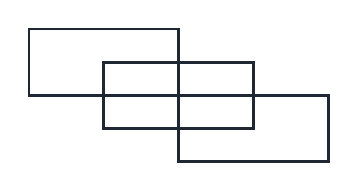
\begin{tikzpicture}[x=0.95cm,y=0.42cm]
\draw[Ink,line width=1pt] (0,2) rectangle (2,4);
\draw[Ink,line width=1pt] (1,1) rectangle (3,3);
\draw[Ink,line width=1pt] (2,0) rectangle (4,2);
\end{tikzpicture}
\end{minipage}
\end{probbox}
\probsol{
\textbf{Phân tích đề.} Ba hình chữ nhật bằng nhau, gọi là \textbf{I} (trên--trái), \textbf{II} (giữa) và \textbf{III} (dưới--phải). Các cạnh cắt nhau tạo ra thêm nhiều hình chữ nhật nhỏ. Ta phải đếm \emph{tất cả} các hình chữ nhật có đủ bốn cạnh được vẽ trên hình.
\step{1}{Quan sát kỹ hình vẽ}
Đặt tên các điểm như hình dưới. Để ý: cạnh dưới của hình I và cạnh trên của hình III nằm trên \emph{cùng một đường thẳng} và nối tiếp nhau tại điểm $O$ -- tâm của hình II. Tương tự cạnh phải của hình I và cạnh trái của hình III nối tiếp nhau tại $O$. Vì vậy bên trong hình II có một ``dấu cộng'' chia hình II thành $4$ ô nhỏ bằng nhau.
\begin{center}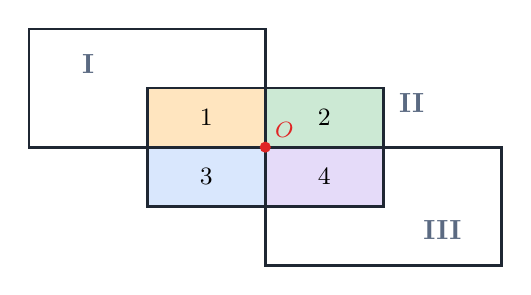
\begin{tikzpicture}[x=1.5cm,y=0.75cm,font=\sffamily\small]
\fill[tmOrange!25] (1,2) rectangle (2,3);\fill[tmGreen!25] (2,2) rectangle (3,3);
\fill[tmBlue!20] (1,1) rectangle (2,2);\fill[tmPurple!20] (2,1) rectangle (3,2);
\draw[Ink,line width=1pt] (0,2) rectangle (2,4);
\draw[Ink,line width=1pt] (1,1) rectangle (3,3);
\draw[Ink,line width=1pt] (2,0) rectangle (4,2);
\node at (1.5,2.5){$1$};\node at (2.5,2.5){$2$};\node at (1.5,1.5){$3$};\node at (2.5,1.5){$4$};
\fill[AnsRed] (2,2) circle (2pt);\node[above right,font=\footnotesize\bfseries,text=AnsRed] at (2,2){$O$};
\node[font=\bfseries,text=Slate] at (0.5,3.4){I};\node[font=\bfseries,text=Slate] at (3.5,0.6){III};
\node[font=\bfseries,text=Slate,anchor=west] at (3.05,2.75){II};
\end{tikzpicture}\end{center}
\step{2}{Đếm theo từng loại}
\begin{itemize}[leftmargin=1.2em,itemsep=1pt,topsep=1pt]
\item \textbf{Ba hình chữ nhật lớn ban đầu:} I, II, III -- $3$ hình.
\item \textbf{Bốn ô nhỏ} trong hình II (ô $1$, $2$, $3$, $4$) -- $4$ hình. Mỗi ô đều có đủ bốn cạnh: ví dụ ô $1$ có cạnh trên và cạnh trái là cạnh của hình II, cạnh dưới và cạnh phải là cạnh của hình I.
\item \textbf{Nửa hình II} (ghép hai ô cạnh nhau): ô $1+2$ (nửa trên), ô $3+4$ (nửa dưới), ô $1+3$ (nửa trái), ô $2+4$ (nửa phải) -- $4$ hình.
\end{itemize}
\step{3}{Kiểm tra không còn hình nào khác}
\begin{itemize}[leftmargin=1.2em,itemsep=1pt,topsep=1pt]
\item Phần của hình I nằm \emph{ngoài} hình II có dạng chữ L, và không có đoạn kẻ nào đi xuyên qua vùng đó. Một hình chữ nhật muốn chứa một phần vùng chữ L này thì phải lấy cạnh trái và cạnh trên của hình I làm cạnh của nó; hai cạnh này chỉ dài đúng bằng cạnh của hình I, nên hình chữ nhật đó chính là hình I. Tương tự, hình chữ nhật chứa một phần của III nằm ngoài II chỉ có thể là hình III.
\item Mọi hình chữ nhật còn lại phải nằm gọn trong hình II. Hình II cùng ``dấu cộng'' bên trong là một lưới $2\times2$ ô, và ở bước 2 ta đã kể đủ: $4$ ô, $4$ nửa và chính hình II.
\end{itemize}
\begin{warnbox}Đừng đếm hình chữ nhật lớn bao quanh cả ba hình (từ góc trên-trái của I đến góc dưới-phải của III): hình đó \emph{không} có cạnh nào được vẽ đầy đủ. Và cũng đừng bỏ sót các ô nhỏ do ``dấu cộng'' ở tâm tạo ra.\end{warnbox}
\step{4}{Cộng lại}
$3+4+4=11$ hình chữ nhật.
\verify{Đếm cách khác -- chỉ trong hình II (đây là một lưới $2\times2$ đầy đủ): theo Ví dụ 7 có $9$ hình chữ nhật (gồm $4$ ô, $4$ nửa và chính hình II). Cộng thêm hình I và hình III: $9+2=11$ \checkmark.}
Đáp án là \textbf{(A)}.
\ans{(A) $11$}
}

% ---------------- part b ----------------
% ================= Topic 3 (VI) -- part b: problems 16--30 =================
\providecommand{\cpTooth}[3]{% #1 rows, #2 columns, #3 unit (cm): grid of toothpicks
  \foreach \j in {0,...,#1}{\foreach \i in {1,...,#2}{
    \draw[tmOrange!85!black,line width=1.6pt,line cap=round]
      ({(\i-1)*#3+0.05},{\j*#3})--({\i*#3-0.05},{\j*#3});}}
  \foreach \j in {1,...,#1}{\foreach \i in {0,...,#2}{
    \draw[tmOrange!85!black,line width=1.6pt,line cap=round]
      ({\i*#3},{(\j-1)*#3+0.05})--({\i*#3},{\j*#3-0.05});}}}

\begin{probbox}{16}{\relax}
Trên lưới điểm ở hình bên, bạn Lan đứng ở điểm $A$. Lan tung một đồng xu cân đối để quyết định
cách di chuyển: nếu đồng xu ra mặt \emph{sấp} thì Lan đi \emph{lên} một điểm; nếu ra mặt \emph{ngửa}
thì Lan đi \emph{sang phải} một điểm. Sau đúng bốn lần tung, Lan sẽ dừng ở một trong năm điểm
$P$, $Q$, $R$, $S$, $T$. Xác suất để Lan dừng ở điểm $R$ là bao nhiêu?
\begin{figC}\begin{scope}[scale=0.8]
  \foreach \y in {0,...,4}{\pgfmathtruncatemacro\m{4-\y}
    \foreach \x in {0,...,\m}{\fill[Navy] (\x,\y) circle (2.6pt);}}
  \node[below left] at (0,0) {$A$};
  \node[above right] at (0,4) {$P$};\node[above right] at (1,3) {$Q$};
  \node[above right] at (2,2) {$R$};\node[above right] at (3,1) {$S$};
  \node[above right] at (4,0) {$T$};
  \fill[tmOrange] (0,0) circle (3.4pt);
\end{scope}\end{figC}
\choices{$\dfrac12$}{$\dfrac38$}{$\dfrac9{16}$}{$\dfrac7{16}$}{$\dfrac5{16}$}
\end{probbox}
\probsol{
\textbf{Phân tích đề.} Mỗi lần tung, Lan đi \emph{lên} ($\uparrow$, khi ra sấp) hoặc \emph{sang phải}
($\rightarrow$, khi ra ngửa). Sau $4$ lần tung, Lan đi đúng $4$ bước. Ta cần tính xác suất để
sau $4$ bước Lan đứng ở $R$.

\step{1}{Đếm tất cả các kết quả có thể}
Mỗi lần tung có $2$ kết quả (sấp hoặc ngửa), bốn lần tung liên tiếp cho
$2\times2\times2\times2=16$ dãy kết quả, ví dụ $\uparrow\rightarrow\rightarrow\uparrow$.
Vì đồng xu cân đối nên $16$ dãy này \emph{đồng khả năng}.
\begin{recallbox}\emph{Quy tắc nhân:} nếu việc thứ nhất có $a$ cách, việc thứ hai có $b$ cách, \dots{} thì
làm lần lượt các việc đó có $a\times b\times\cdots$ cách. \emph{Xác suất} của một biến cố (khi các kết
quả đồng khả năng) $=\dfrac{\text{số kết quả thuận lợi}}{\text{số kết quả có thể}}$.\end{recallbox}

\step{2}{Điểm cuối chỉ phụ thuộc vào số bước đi lên}
Nếu trong $4$ bước có $k$ bước đi lên thì có $4-k$ bước sang phải. Thứ tự các bước không làm thay
đổi điểm cuối. Đặt $A$ là gốc, ta có: $4$ lần lên $\to P$; $3$ lần lên $\to Q$;
$2$ lần lên $\to R$; $1$ lần lên $\to S$; $0$ lần lên $\to T$.
Vậy Lan dừng ở $R$ khi và chỉ khi có \textbf{đúng $2$ bước lên và $2$ bước sang phải}.

\step{3}{Liệt kê các dãy thuận lợi}
Ta chọn vị trí của hai bước $\uparrow$ trong bốn lượt (lượt 1, 2, 3, 4):
\[\uparrow\uparrow\rightarrow\rightarrow,\quad \uparrow\rightarrow\uparrow\rightarrow,\quad
\uparrow\rightarrow\rightarrow\uparrow,\quad \rightarrow\uparrow\uparrow\rightarrow,\quad
\rightarrow\uparrow\rightarrow\uparrow,\quad \rightarrow\rightarrow\uparrow\uparrow.\]
Có $6$ dãy (chọn $2$ lượt trong $4$ lượt: $\dfrac{4\times3}{2}=6$ cách).

\step{4}{Tính xác suất}
\[P(\text{dừng ở } R)=\frac{6}{16}=\frac38.\]

\step{5}{Một cách nhìn bằng hình: ghi số đường đi tới mỗi điểm}
Ghi vào mỗi điểm số dãy bước dẫn từ $A$ tới điểm đó. Mỗi điểm chỉ có thể tới từ điểm ngay bên trái hoặc
ngay bên dưới, nên số ở mỗi điểm $=$ tổng hai số ở bên trái và bên dưới (giống tam giác Pascal):
\begin{figC}\begin{scope}[scale=0.75]
  \foreach \x/\y/\n in {0/0/1,1/0/1,2/0/1,3/0/1,4/0/1,0/1/1,1/1/2,2/1/3,3/1/4,0/2/1,1/2/3,2/2/6,
     0/3/1,1/3/4,0/4/1}{
    \fill[tmBlue!12] (\x,\y) circle (9pt);
    \node[font=\small\bfseries,text=Navy] at (\x,\y) {\n};}
  \draw[AnsRed,thick] (2,2) circle (10pt);
  \node[right=10pt,text=AnsRed,font=\small] at (2,2) {$R$};
  \node[right=10pt,font=\small] at (4,0) {$T$};\node[right=10pt,font=\small] at (3,1) {$S$};
  \node[right=10pt,font=\small] at (1,3) {$Q$};\node[right=10pt,font=\small] at (0,4) {$P$};
\end{scope}\end{figC}
Trên đường chéo cuối: $1+4+6+4+1=16$ (đúng bằng tổng số dãy) và tại $R$ có số $6$.
\begin{warnbox}Năm điểm $P,Q,R,S,T$ \emph{không} đồng khả năng! Không được trả lời ``$1$ trong $5$ điểm nên
xác suất là $\frac15$''. Điểm ở giữa ($R$) có nhiều đường đi tới nhất; hai điểm ở đầu ($P$ và $T$) mỗi điểm chỉ có một đường.\end{warnbox}
\verify{Xác suất dừng ở các điểm $P,Q,R,S,T$ lần lượt là $\frac1{16},\frac4{16},\frac6{16},\frac4{16},\frac1{16}$;
tổng bằng $\frac{16}{16}=1$, hợp lý.}
Giá trị $\frac38=\frac6{16}$ là phương án \textbf{(B)}.
\ans{(B) $\dfrac38$}
}

\begin{probbox}{17}{\relax}
Người ta dùng các que tăm giống hệt nhau để xếp thành các lưới ô vuông như hình dưới. Chẳng hạn, lưới
$1\times10$ (gồm $1$ hàng, $10$ cột ô vuông) cần tất cả $31$ que tăm. Hỏi để xếp lưới $43\times10$
($43$ hàng, mỗi hàng $10$ ô) thì cần bao nhiêu que tăm?
\begin{figC}
  \begin{scope}[shift={(0,2.4)}]\cpTooth{1}{10}{0.42}\node[right] at (4.4,0.21) {$1\times10$};\end{scope}
  \begin{scope}[shift={(0,1.05)}]\cpTooth{2}{10}{0.42}\node[right] at (4.4,0.42) {$2\times10$};\end{scope}
  \begin{scope}[shift={(0,-0.6)}]\cpTooth{3}{10}{0.42}\node[right] at (4.4,0.63) {$3\times10$};\end{scope}
\end{figC}
\choices{$913$}{$860$}{$871$}{$903$}{$946$}
\end{probbox}
\probsol{
\textbf{Phân tích đề.} Lưới $43\times10$ có $43$ hàng ô vuông, mỗi hàng $10$ ô. Các que tăm nằm theo hai
hướng: \emph{nằm ngang} và \emph{thẳng đứng}. Ta đếm riêng từng loại rồi cộng lại (quy tắc cộng).

\step{1}{Kiểm tra cách đếm trên lưới $1\times10$}
\emph{Que nằm ngang:} lưới có $2$ đường kẻ ngang (cạnh trên và cạnh dưới), mỗi đường gồm $10$ que:
$2\times10=20$ que.
\emph{Que thẳng đứng:} có $11$ đường kẻ dọc ($10$ ô cần $11$ vách ngăn), mỗi đường gồm $1$ que:
$11\times1=11$ que. Tổng: $20+11=31$ que, đúng như đề cho.
\begin{recallbox}Một hàng có $10$ ô thì cần $10+1=11$ vách dọc (giống bài toán trồng cây: $10$ khoảng cách
thì có $11$ cây). Tương tự, $43$ hàng ô thì có $43+1=44$ đường kẻ ngang.\end{recallbox}

\step{2}{Đếm que nằm ngang của lưới $43\times10$}
Có $43+1=44$ đường kẻ ngang, mỗi đường dài $10$ que: $44\times10=440$ que.

\step{3}{Đếm que thẳng đứng của lưới $43\times10$}
Có $10+1=11$ đường kẻ dọc, mỗi đường dài $43$ que (mỗi hàng ô góp $1$ que): $11\times43=473$ que.

\step{4}{Cộng lại}
$440+473=913$ que tăm.

\step{5}{Cách thứ hai: thêm từng hàng}
Lưới $1\times10$ có $31$ que. Mỗi khi đặt thêm một hàng mới lên trên, ta cần thêm $10$ que nằm ngang
(cạnh trên của hàng mới) và $11$ que thẳng đứng, tức $21$ que (cạnh dưới đã có sẵn). Từ $1$ hàng lên
$43$ hàng phải thêm $42$ hàng:
\[31+42\times21=31+882=913.\]
\begin{warnbox}Không được lấy $43\times31=1333$: khi chồng các hàng lên nhau, hai hàng kề nhau \emph{dùng chung}
một dãy $10$ que nằm ngang, nên nhân như vậy là đếm trùng.\end{warnbox}
\verify{Theo công thức $(\text{số hàng}+1)\times10+11\times\text{số hàng}$: lưới $2\times10$ cần
$3\times10+11\times2=52$ que, lưới $3\times10$ cần $4\times10+11\times3=73$ que; đếm trực tiếp trên hình cũng
được $52$ và $73$. Hai cách tính cho cùng kết quả $913$.}
Vậy chọn \textbf{(A)}.
\ans{(A) $913$ que tăm}
}

\begin{probbox}{18}{\relax}
Ở căng-tin trường bạn Minh, món thịt có hai loại là thịt bò và thịt gà; trái cây có ba loại là táo, lê
và chuối. Minh được phát ngẫu nhiên một suất ăn gồm một món thịt và một loại trái cây. Xác suất để
suất ăn của Minh có chuối là
\choices{$\dfrac13$}{$\dfrac23$}{$\dfrac12$}{$\dfrac15$}{$\dfrac35$}
\end{probbox}
\probsol{
\textbf{Phân tích đề.} Một suất ăn $=$ (một món thịt, một loại trái cây). Suất ăn được chọn ngẫu nhiên
nên mọi suất ăn có thể đều đồng khả năng. Cần tìm xác suất suất ăn có chuối.

\step{1}{Liệt kê tất cả các suất ăn có thể}
Theo quy tắc nhân có $2\times3=6$ suất ăn. Ta lập bảng (hàng: thịt, cột: trái cây):
\begin{center}\begin{tabular}{|c|c|c|c|}\hline
 & Táo & Lê & \cellcolor{tmOrange!20}Chuối\\\hline
Bò & Bò--Táo & Bò--Lê & \cellcolor{tmOrange!20}Bò--Chuối\\\hline
Gà & Gà--Táo & Gà--Lê & \cellcolor{tmOrange!20}Gà--Chuối\\\hline
\end{tabular}\end{center}

\step{2}{Đếm các suất ăn có chuối}
Cột ``Chuối'' có $2$ suất: Bò--Chuối và Gà--Chuối.

\step{3}{Tính xác suất}
\[P(\text{có chuối})=\frac{2}{6}=\frac13.\]
\begin{recallbox}Rút gọn phân số: chia cả tử và mẫu cho ước chung lớn nhất: $\dfrac26=\dfrac{2:2}{6:2}=\dfrac13$.\end{recallbox}
\begin{tipbox}Món thịt không ảnh hưởng gì tới trái cây. Có thể nghĩ gọn: trái cây được chọn là một trong
$3$ loại đồng khả năng, chuối là $1$ trong $3$ loại, nên xác suất là $\frac13$.\end{tipbox}
\begin{warnbox}Đừng cộng ``$2$ loại thịt $+\,3$ loại trái cây $=5$'' rồi trả lời $\frac15$: số suất ăn là
$2\times3=6$ chứ không phải $2+3=5$.\end{warnbox}
\verify{Xác suất có táo, có lê, có chuối đều bằng $\frac13$; tổng $\frac13+\frac13+\frac13=1$.}
Vậy chọn \textbf{(A)}.
\ans{(A) $\dfrac13$}
}

\begin{probbox}{19}{\relax}
Người ta làm một con xúc xắc đặc biệt có sáu mặt, mỗi mặt ghi một số (các số có thể trùng nhau). Khi gieo
xúc xắc này, xác suất được một số chia hết cho $3$ là $\frac12$, còn xác suất được một số chẵn là $\frac13$.
Sáu số trên các mặt có thể là
\choicesII{$1,2,3,5,5,6$}{$1,2,3,3,5,6$}{$1,2,3,4,6,6$}{$1,2,3,3,4,6$}{$2,3,3,3,5,6$}
\end{probbox}
\probsol{
\textbf{Phân tích đề.} Xúc xắc có $6$ mặt đồng khả năng. Từ hai xác suất đã cho, ta suy ra \emph{số mặt}
ghi số chia hết cho $3$ và số mặt ghi số chẵn, rồi kiểm tra từng phương án.

\step{1}{Đổi xác suất thành số mặt}
\begin{recallbox}Với $6$ mặt đồng khả năng: $P=\dfrac{\text{số mặt thuận lợi}}{6}$, nên
số mặt thuận lợi $=P\times6$.\end{recallbox}
Số mặt chia hết cho $3$: $\frac12\times6=3$ mặt.\quad Số mặt chẵn: $\frac13\times6=2$ mặt.

Vậy ta cần: \textbf{đúng $3$ mặt chia hết cho $3$} và \textbf{đúng $2$ mặt chẵn}.

\step{2}{Kiểm tra từng phương án}
Trong các số từ $1$ đến $6$: các số chia hết cho $3$ là $3$ và $6$; các số chẵn là $2$, $4$, $6$.
Chú ý số $6$ vừa chẵn vừa chia hết cho $3$, nên phải đếm nó ở \emph{cả hai} cột.
\begin{center}\begin{tabular}{|c|c|c|c|c|}\hline
Phương án & Các mặt & Mặt chia hết cho $3$ & Mặt chẵn & Đạt?\\\hline
(A) & $1,2,3,5,5,6$ & $3,6$ \;($2$ mặt) & $2,6$ \;($2$ mặt) & Không\\\hline
\rowcolor{tmGreen!12}(B) & $1,2,3,3,5,6$ & $3,3,6$ \;($3$ mặt) & $2,6$ \;($2$ mặt) & Có\\\hline
(C) & $1,2,3,4,6,6$ & $3,6,6$ \;($3$ mặt) & $2,4,6,6$ \;($4$ mặt) & Không\\\hline
(D) & $1,2,3,3,4,6$ & $3,3,6$ \;($3$ mặt) & $2,4,6$ \;($3$ mặt) & Không\\\hline
(E) & $2,3,3,3,5,6$ & $3,3,3,6$ \;($4$ mặt) & $2,6$ \;($2$ mặt) & Không\\\hline
\end{tabular}\end{center}
\begin{warnbox}Nếu quên rằng $6$ là số chẵn, ta sẽ đếm sai số mặt chẵn của (D) thành $2$ và chọn nhầm (D).
Một số có thể thuộc nhiều nhóm cùng lúc!\end{warnbox}
\verify{Với (B): $P(\text{chia hết cho }3)=\frac36=\frac12$ và $P(\text{chẵn})=\frac26=\frac13$, đúng cả hai điều kiện.}
Chỉ có phương án \textbf{(B)} thoả mãn.
\ans{(B) $1,2,3,3,5,6$}
}

\begin{probbox}{20}{\stars{1}}
Ba tuyến xe buýt chạy trên các con đường như hình vẽ, cùng đi qua bến $X$ (các đoạn có cùng số vạch
nhỏ thì dài bằng nhau: $PX=XS$, $QX=XT$, $RX=XU$).
\begin{itemize}[leftmargin=1.2em,itemsep=1pt,topsep=2pt]
\item Xe $A$ chạy theo lộ trình $P\to X\to S\to X\to P$, mỗi vòng mất $12$ phút.
\item Xe $B$ chạy theo lộ trình $Q\to X\to T\to X\to Q$, mỗi vòng mất $20$ phút.
\item Xe $C$ chạy theo lộ trình $R\to X\to U\to X\to R$, mỗi vòng mất $28$ phút.
\end{itemize}
Lúc $13$\,h, ba xe $A$, $B$, $C$ lần lượt xuất phát từ $P$, $Q$, $R$. Mỗi xe chạy với vận tốc không đổi,
quay đầu ngay lập tức ở hai đầu lộ trình và chạy liên tục đến $23$\,h. Hỏi trong khoảng thời gian từ
$17$\,h đến $22$\,h, có bao nhiêu thời điểm mà có từ hai xe trở lên cùng có mặt tại bến $X$?
\begin{figC}\begin{scope}[scale=0.9]
  \draw[Ink,thick] (0,1.6)--(0,-1.6);\draw[Ink,thick] (-1.9,0)--(1.9,0);\draw[Ink,thick] (-2,-1.35)--(2,1.35);
  \foreach \p in {(0,1.6),(0,-1.6),(-1.9,0),(1.9,0),(-2,-1.35),(2,1.35),(0,0)}{\fill[Navy] \p circle (2pt);}
  \node[above] at (0,1.6) {$P$};\node[below] at (0,-1.6) {$S$};\node[left] at (-1.9,0) {$Q$};
  \node[right] at (1.9,0) {$T$};\node[below left] at (-2,-1.35) {$R$};\node[above right] at (2,1.35) {$U$};
  \node[below right] at (0.05,-0.02) {$X$};
  % ticks
  \draw[tmBlue,thick] (-0.12,0.8)--(0.12,0.8);\draw[tmBlue,thick] (-0.12,-0.8)--(0.12,-0.8);
  \foreach \s in {-1,1}{\draw[tmOrange,thick] (\s*0.95-0.04,-0.12)--(\s*0.95-0.04,0.12);
                        \draw[tmOrange,thick] (\s*0.95+0.04,-0.12)--(\s*0.95+0.04,0.12);}
  \foreach \s in {-1,1}{\foreach \d in {-0.09,0,0.09}{
     \draw[tmGreen!80!black,thick] ($(\s*1,\s*0.675)+(\d*0.829,\d*0.559)+(0.067,-0.1)$)--++(-0.134,0.2);}}
\end{scope}\end{figC}
\choices{$18$}{$19$}{$20$}{$21$}{$22$}
\end{probbox}
\probsol{
\textbf{Phân tích đề.} Ta đo thời gian bằng \emph{số phút kể từ $13$\,h} và gọi số đó là $t$. Cần tìm
những giá trị $t$ mà có ít nhất hai xe cùng ở $X$, với $t$ nằm trong khoảng từ $17$\,h đến $22$\,h.

\step{1}{Đổi khoảng thời gian cần xét ra số phút}
$17$\,h là $4$ giờ sau $13$\,h: $t=4\times60=240$. \quad $22$\,h là $9$ giờ sau $13$\,h: $t=9\times60=540$.
Vậy ta xét $240\le t\le540$.

\step{2}{Xe $A$ có mặt ở $X$ vào những lúc nào?}
Một vòng của xe $A$ gồm $4$ đoạn bằng nhau: $P\to X$, $X\to S$, $S\to X$, $X\to P$ (vì $PX=XS$).
Xe chạy đều nên mỗi đoạn mất $12:4=3$ phút. Xe $A$ tới $X$ ở cuối đoạn thứ nhất và cuối đoạn thứ ba
của mỗi vòng, tức là lúc
\[t=3,\ 9,\ 15,\ 21,\ 27,\ \dots\]
Đó chính là các \textbf{bội lẻ của $3$} ($3\times1$, $3\times3$, $3\times5$, \dots). Ở cuối đoạn thứ hai và thứ tư
xe ở $S$ hoặc $P$, không ở $X$.

\step{3}{Tương tự với xe $B$ và xe $C$}
Xe $B$: mỗi đoạn mất $20:4=5$ phút, xe ở $X$ lúc $t=5,15,25,35,\dots$ -- các \textbf{bội lẻ của $5$}.\\
Xe $C$: mỗi đoạn mất $28:4=7$ phút, xe ở $X$ lúc $t=7,21,35,49,\dots$ -- các \textbf{bội lẻ của $7$}.

\step{4}{Khi nào hai xe gặp nhau ở $X$?}
\begin{recallbox}Một số chia hết cho cả $3$ và $5$ thì chia hết cho $\text{BCNN}(3,5)=15$. Tương tự:
chia hết cho cả $3$ và $7$ $\Leftrightarrow$ chia hết cho $21$; chia hết cho cả $5$ và $7$ $\Leftrightarrow$
chia hết cho $35$.\end{recallbox}
Xe $A$ và xe $B$ cùng ở $X$ khi $t$ vừa là bội lẻ của $3$ vừa là bội lẻ của $5$, tức $t$ là \textbf{số lẻ chia hết cho $15$}
(bội lẻ của $15$). Tương tự: $A$ và $C$ gặp nhau khi $t$ là bội lẻ của $21$; $B$ và $C$ gặp nhau khi $t$ là bội lẻ của $35$.
\begin{proofbox}Bội lẻ của $15$ là số lẻ chia hết cho $15$, nên nó vừa là số lẻ chia hết cho $3$ (bội lẻ của $3$), vừa là
số lẻ chia hết cho $5$ (bội lẻ của $5$). Ngược lại, một số vừa là bội lẻ của $3$ vừa là bội lẻ của $5$ thì lẻ và chia
hết cho $15$.\end{proofbox}

\step{5}{Liệt kê trong khoảng $240\le t\le540$}
\begin{center}\begin{tabular}{|l|l|c|}\hline
Hai xe & Các giá trị $t$ (bội lẻ) & Số lần\\\hline
$A$ và $B$ ($15$) & $255, 285, 315, 345, 375, 405, 435, 465, 495, 525$ & $10$\\\hline
$A$ và $C$ ($21$) & $273, 315, 357, 399, 441, 483, 525$ & $7$\\\hline
$B$ và $C$ ($35$) & $245, 315, 385, 455, 525$ & $5$\\\hline
\end{tabular}\end{center}
(Ví dụ hàng đầu: $15\times17=255$ là bội lẻ đầu tiên lớn hơn $240$; sau đó cứ cộng thêm $30$, vì giữa hai
bội lẻ liên tiếp của $15$ cách nhau $2\times15=30$.)

\step{6}{Bỏ các thời điểm bị đếm trùng}
Cộng ba hàng được $10+7+5=22$, nhưng các thời điểm $315$ và $525$ xuất hiện ở \emph{cả ba hàng}
(đó là bội lẻ của $3\times5\times7=105$: lúc ấy cả ba xe cùng ở $X$). Mỗi thời điểm này bị đếm $3$ lần
trong khi chỉ được đếm $1$ lần, nên phải bớt $2+2=4$:
\[22-4=18 \text{ thời điểm.}\]
\begin{warnbox}Đề hỏi số \emph{thời điểm}, không phải số ``cặp xe gặp nhau''. Lúc ba xe cùng ở $X$ chỉ là
\emph{một} thời điểm. Cộng thẳng $10+7+5=22$ rồi chọn (E) là sai.\end{warnbox}
\verify{Đổi ra giờ: $17$\,h\,05; $17$\,h\,15; $17$\,h\,33; $17$\,h\,45; $18$\,h\,15; $18$\,h\,45; $18$\,h\,57;
$19$\,h\,15; $19$\,h\,25; $19$\,h\,39; $19$\,h\,45; $20$\,h\,15; $20$\,h\,21; $20$\,h\,35; $20$\,h\,45; $21$\,h\,03;
$21$\,h\,15; $21$\,h\,45 -- đếm được đúng $18$ thời điểm, tất cả đều nằm giữa $17$\,h và $22$\,h.}
Vậy chọn \textbf{(A)}.
\ans{(A) $18$}
}

\begin{probbox}{21}{\relax}
Mỗi mặt của một hình lập phương được sơn đúng một màu. Cần ít nhất bao nhiêu màu để sơn hình lập
phương sao cho hai mặt bất kì có chung một cạnh thì có màu khác nhau?
\choices{$2$}{$3$}{$4$}{$5$}{$6$}
\end{probbox}
\probsol{
\textbf{Phân tích đề.} Hai mặt ``có chung một cạnh'' là hai mặt kề nhau. Hai mặt đối diện (như mặt trên và
mặt dưới) không có cạnh chung nên được phép cùng màu. Ta cần (1) chỉ ra một cách tô dùng ít màu, và
(2) chứng minh không thể dùng ít màu hơn.

\step{1}{Hai màu là không đủ}
\begin{proofbox}Xét một đỉnh bất kì của hình lập phương, chẳng hạn đỉnh trên--trước--phải. Có ba mặt gặp nhau ở
đỉnh đó: mặt trên, mặt trước, mặt phải. Hai mặt bất kì trong ba mặt này đều có chung một cạnh, nên ba mặt
này phải có ba màu đôi một khác nhau. Do đó cần ít nhất $3$ màu.\end{proofbox}

\step{2}{Ba màu là đủ}
Tô \emph{hai mặt đối diện cùng một màu}: mặt trên và mặt dưới màu xanh dương, mặt trước và mặt sau màu
cam, mặt trái và mặt phải màu xanh lá. Mỗi mặt kề với $4$ mặt, đó chính là bốn mặt \emph{không} đối diện
với nó, và bốn mặt này mang hai màu kia. Vậy không có hai mặt kề nhau nào cùng màu.
\begin{figC}
  \begin{scope}
   \fill[tmOrange!55,draw=Ink,thick] (0,0)--(1.6,0)--(1.6,1.6)--(0,1.6)--cycle;
   \fill[tmBlue!55,draw=Ink,thick] (0,1.6)--(1.6,1.6)--(2.4,2.3)--(0.8,2.3)--cycle;
   \fill[tmGreen!55,draw=Ink,thick] (1.6,0)--(2.4,0.7)--(2.4,2.3)--(1.6,1.6)--cycle;
   \node at (0.8,0.8) {trước};\node at (1.2,1.95) {trên};\node[rotate=0] at (2,1.15) {phải};
  \end{scope}
  \begin{scope}[shift={(4,0.1)},scale=0.5]
   \foreach \x/\y/\c in {1/2/tmBlue,0/1/tmGreen,1/1/tmOrange,2/1/tmGreen,3/1/tmOrange,1/0/tmBlue}{
     \fill[\c!55,draw=Ink,thick] (\x,\y) rectangle ++(1,1);}
   \node[font=\scriptsize] at (2,-0.45) {hình khai triển};
  \end{scope}
\end{figC}

\step{3}{Kết luận}
Cần ít nhất $3$ màu (bước 1) và $3$ màu là đủ (bước 2), nên số màu nhỏ nhất là $3$.
\begin{warnbox}Chỉ tìm được một cách tô bằng $3$ màu thì \emph{chưa đủ} để khẳng định $3$ là nhỏ nhất; phải
giải thích vì sao $2$ màu không được (lập luận ba mặt chung đỉnh). Ngược lại, nghĩ rằng ``$6$ mặt phải có
$6$ màu'' là quên rằng mặt đối diện được phép cùng màu.\end{warnbox}
\verify{Trên hình khai triển, mỗi ô vuông chỉ chung cạnh với các ô khác màu (khi gấp lại, hai ô cùng màu
là hai mặt đối diện).}
Vậy chọn \textbf{(B)}.
\ans{(B) $3$ màu}
}

\begin{probbox}{22}{\relax}
Có bao nhiêu cặp số $(m,n)$ khác nhau lấy từ các số nguyên $1,2,3,\dots,20$ sao cho $m<n$ và $m+n$ là số chẵn?
\choices{$55$}{$90$}{$140$}{$110$}{$50$}
\end{probbox}
\probsol{
\textbf{Phân tích đề.} Ta chọn hai số khác nhau trong $20$ số; vì yêu cầu $m<n$ nên mỗi cặp hai số chỉ được
đếm \emph{một lần} (số nhỏ là $m$, số lớn là $n$). Điều kiện: tổng $m+n$ chẵn.

\step{1}{Khi nào tổng hai số là số chẵn?}
\begin{recallbox}chẵn $+$ chẵn $=$ chẵn;\quad lẻ $+$ lẻ $=$ chẵn;\quad chẵn $+$ lẻ $=$ lẻ.\end{recallbox}
Vậy $m+n$ chẵn khi và chỉ khi $m$ và $n$ \textbf{cùng tính chẵn lẻ} (cùng chẵn hoặc cùng lẻ).

\step{2}{Chia $20$ số thành hai nhóm}
Nhóm chẵn: $2,4,6,\dots,20$ -- có $10$ số.\quad Nhóm lẻ: $1,3,5,\dots,19$ -- có $10$ số.

\step{3}{Đếm số cặp trong nhóm chẵn}
Chọn số thứ nhất có $10$ cách, số thứ hai (khác số thứ nhất) có $9$ cách: $10\times9=90$ cách chọn \emph{có thứ tự}.
Nhưng mỗi cặp, ví dụ $\{2,4\}$, bị đếm hai lần ($2$ rồi $4$, hoặc $4$ rồi $2$), trong khi điều kiện $m<n$
chỉ cho phép một thứ tự $(2,4)$. Vậy số cặp là $\dfrac{10\times9}{2}=45$.
\begin{recallbox}Số cách chọn $2$ phần tử (không kể thứ tự) từ $k$ phần tử là $\dfrac{k\times(k-1)}{2}$.\end{recallbox}

\step{4}{Đếm số cặp trong nhóm lẻ và cộng lại}
Tương tự, nhóm lẻ cho $45$ cặp. Một cặp không thể vừa ở nhóm chẵn vừa ở nhóm lẻ, nên theo quy tắc cộng:
$45+45=90$ cặp.
\begin{warnbox}Quên chia cho $2$ sẽ được $90+90=180$ (không có trong đáp án); quên mất nhóm lẻ sẽ được
$45$. Hãy luôn tự hỏi: ``Mình có đếm một cặp hai lần không? Mình có bỏ sót trường hợp nào không?''\end{warnbox}
\verify{Đếm bằng phần bù: tổng số cặp $m<n$ là $\dfrac{20\times19}{2}=190$. Số cặp khác tính chẵn lẻ (một chẵn, một lẻ) là
$10\times10=100$. Vậy số cặp cùng tính chẵn lẻ là $190-100=90$. Khớp!}
Vậy chọn \textbf{(B)}.
\ans{(B) $90$ cặp}
}

\begin{probbox}{23}{\stars{1}}
Hai số nguyên dương có hai chữ số, khác nhau, được gọi là một \emph{cặp số đảo} nếu số này nhận được từ số kia bằng
cách đổi chỗ hai chữ số. Ví dụ: $52$ và $25$ là một cặp số đảo. Số $2015$ có một tính chất đặc biệt: nó bằng
tích của ba số nguyên tố khác nhau, trong đó có hai số tạo thành một cặp số đảo ($2015=5\times13\times31$).
Kể cả $2015$, có bao nhiêu số nguyên dương nhỏ hơn $10\,000$ có cùng tính chất này?
\choices{$18$}{$14$}{$20$}{$17$}{$19$}
\end{probbox}
\probsol{
\textbf{Phân tích đề.} Ta cần đếm các số $N<10\,000$ có dạng $N=p\times q\times r$, với $p,q,r$ là ba số nguyên
tố khác nhau, trong đó hai số (gọi là $p$ và $q$) là một cặp số đảo có hai chữ số. Kế hoạch: tìm tất cả các
cặp số đảo gồm hai số nguyên tố, rồi với mỗi cặp tìm các số nguyên tố thứ ba phù hợp.

\step{1}{Tìm các cặp số đảo mà cả hai số đều là số nguyên tố}
\begin{recallbox}Số nguyên tố là số tự nhiên lớn hơn $1$ chỉ có hai ước là $1$ và chính nó. Các số nguyên tố có
hai chữ số: $11, 13, 17, 19, 23, 29, 31, 37, 41, 43, 47, 53, 59, 61, 67, 71, 73, 79, 83, 89, 97$.\end{recallbox}
\begin{tipbox}Số đảo của $p$ có chữ số hàng đơn vị chính là chữ số hàng chục của $p$. Số nguyên tố có hai chữ số
phải tận cùng bằng $1,3,7$ hoặc $9$, nên chỉ cần xét các số nguyên tố bắt đầu bằng $1,3,7,9$:
$11,13,17,19,31,37,71,73,79,97$.\end{tipbox}
Kiểm tra số đảo của từng số:
\begin{center}\begin{tabular}{|c|c|c|c|c|c|c|c|c|c|c|}\hline
$p$ & $11$ & $13$ & $17$ & $19$ & $31$ & $37$ & $71$ & $73$ & $79$ & $97$\\\hline
số đảo & $11$ & $31$ & $71$ & $91$ & $13$ & $73$ & $17$ & $37$ & $97$ & $79$\\\hline
nguyên tố? & trùng & có & có & không & có & có & có & có & có & có\\\hline
\end{tabular}\end{center}
($91=7\times13$ không là số nguyên tố; $11$ đảo lại vẫn là $11$, không phải hai số \emph{khác nhau}.)
Vậy có đúng $4$ cặp: $\{13,31\}$, $\{17,71\}$, $\{37,73\}$, $\{79,97\}$.

\step{2}{Tính tích của mỗi cặp}
$13\times31=403$;\quad $17\times71=1207$;\quad $37\times73=2701$;\quad $79\times97=7663$.

\step{3}{Tìm số nguyên tố thứ ba $r$ cho từng cặp}
Cần $r$ là số nguyên tố, khác hai số của cặp, và tích $<10\,000$.
\begin{itemize}[leftmargin=1.2em,itemsep=1pt,topsep=2pt]
\item Cặp $\{13,31\}$: cần $403\times r<10\,000$. Vì $403\times24=9672$ và $403\times25=10\,075$ nên $r\le23$.
Các số nguyên tố $\le23$ là $2,3,5,7,11,13,17,19,23$; bỏ $13$ (đã có trong cặp): còn $8$ số, cho
$806;\ 1209;\ 2015;\ 2821;\ 4433;\ 6851;\ 7657;\ 9269$.
\item Cặp $\{17,71\}$: cần $1207\times r<10\,000$, mà $1207\times8=9656$, $1207\times9=10\,863$ nên $r\le8$:
$r\in\{2,3,5,7\}$, cho $2414;\ 3621;\ 6035;\ 8449$ ($4$ số).
\item Cặp $\{37,73\}$: $2701\times3=8103<10\,000$, $2701\times4>10\,000$ nên $r\in\{2,3\}$: $5402;\ 8103$ ($2$ số).
\item Cặp $\{79,97\}$: ngay cả $7663\times2=15\,326>10\,000$, nên không có số nào.
\end{itemize}

\step{4}{Kiểm tra không có số nào bị đếm hai lần và cộng lại}
\begin{proofbox}Mỗi số chỉ có một cách phân tích ra thừa số nguyên tố. Nếu một số xuất hiện ở hai danh sách thì
trong ba thừa số nguyên tố của nó có hai cặp số đảo khác nhau; hai cặp này phải dùng chung một số nguyên tố.
Nhưng nhìn bảng ở bước 1, mỗi số nguyên tố chỉ thuộc đúng một cặp. Vậy không có số nào bị đếm hai lần.\end{proofbox}
Tổng cộng: $8+4+2+0=14$ số.
\begin{warnbox}Hai lỗi hay gặp: (1) quên rằng số thứ ba phải \emph{khác} hai số của cặp, nên đếm thêm
$403\times13=5239=13\times13\times31$ (sai, vì $13$ lặp lại); (2) quên số nguyên tố $2$.\end{warnbox}
\verify{$2015=403\times5$ có trong danh sách. Kiểm tra vài số: $9269=13\times31\times23$, $8449=17\times71\times7$,
$8103=37\times73\times3$; tất cả đều nhỏ hơn $10\,000$.}
Vậy chọn \textbf{(B)}.
\ans{(B) $14$}
}

\begin{probbox}{24}{\relax}
Hình bên được ghép từ $8$ hình bình hành nhỏ giống hệt nhau. Kể cả $8$ hình bình hành nhỏ đó, trong
hình có tất cả bao nhiêu hình bình hành?
\begin{figC}
  \foreach \j in {0,1,2}{\draw[Ink,thick] (\j*0.55,\j*0.8)--(4.4+\j*0.55,\j*0.8);}
  \foreach \i in {0,...,4}{\draw[Ink,thick] (\i*1.1,0)--(\i*1.1+1.1,1.6);}
\end{figC}
\choices{$29$}{$30$}{$26$}{$27$}{$28$}
\end{probbox}
\probsol{
\textbf{Phân tích đề.} Hình gồm $2$ hàng, mỗi hàng $4$ hình bình hành nhỏ. Mỗi hình bình hành trong hình được
tạo bởi các đoạn thẳng có sẵn: hai cạnh nằm trên \emph{đường nằm ngang}, hai cạnh nằm trên \emph{đường xiên}.

\step{1}{Đếm các đường thẳng của hình}
Đánh số: có $3$ đường nằm ngang (đáy, giữa, trên) và $5$ đường xiên (song song với nhau).
\begin{figC}
  \foreach \j/\l in {0/1,1/2,2/3}{\draw[tmBlue,thick] (\j*0.55,\j*0.8)--(4.4+\j*0.55,\j*0.8);
     \node[left,text=tmBlue,font=\scriptsize] at (\j*0.55,\j*0.8) {ngang \l};}
  \foreach \i in {0,...,4}{\draw[tmOrange,thick] (\i*1.1,0)--(\i*1.1+1.1,1.6);
     \pgfmathtruncatemacro\k{\i+1}\node[below,text=tmOrange!80!black,font=\scriptsize] at (\i*1.1,0) {x\k};}
  \fill[tmGreen!30,opacity=0.7] (1.1,0)--(3.3,0)--(3.85,0.8)--(1.65,0.8)--cycle;
\end{figC}
Ví dụ: hình bình hành tô xanh lá được xác định bởi đường ngang $1$, ngang $2$ và đường xiên x$2$, x$4$.

\step{2}{Mỗi hình bình hành ứng với một cách chọn $2$ đường ngang và $2$ đường xiên}
Chọn $2$ trong $3$ đường ngang làm cạnh dưới và cạnh trên, chọn $2$ trong $5$ đường xiên làm cạnh trái và cạnh phải,
ta được đúng một hình bình hành; ngược lại mỗi hình bình hành trong hình cho đúng một cách chọn như vậy.
\begin{recallbox}Số cách chọn $2$ đường trong $k$ đường là $\dfrac{k\times(k-1)}{2}$.\end{recallbox}
Chọn $2$ đường ngang: $\dfrac{3\times2}{2}=3$ cách. \quad Chọn $2$ đường xiên: $\dfrac{5\times4}{2}=10$ cách.

\step{3}{Áp dụng quy tắc nhân}
Số hình bình hành: $3\times10=30$.

\step{4}{Kiểm tra bằng cách đếm theo kích thước}
Gọi hình bình hành ``cao $a$, rộng $b$'' là hình gồm $a$ hàng và $b$ cột hình nhỏ:
\begin{center}\begin{tabular}{|c|c|c|c|c|c|}\hline
 & rộng $1$ & rộng $2$ & rộng $3$ & rộng $4$ & Cộng\\\hline
cao $1$ (có $2$ vị trí theo hàng) & $2\times4=8$ & $2\times3=6$ & $2\times2=4$ & $2\times1=2$ & $20$\\\hline
cao $2$ (có $1$ vị trí theo hàng) & $4$ & $3$ & $2$ & $1$ & $10$\\\hline
\end{tabular}\end{center}
\begin{warnbox}Đừng chỉ đếm $8$ hình nhỏ cộng vài hình lớn ``dễ thấy''. Hãy đếm có hệ thống: theo kích thước
(bảng trên) hoặc theo cách chọn các đường thẳng.\end{warnbox}
\verify{Tổng theo bảng: $20+10=30$, trùng với cách tính $3\times10$.}
Vậy chọn \textbf{(B)}.
\ans{(B) $30$ hình bình hành}
}

\begin{probbox}{25}{\stars{1}}
Trong một cái lọ có $2$ viên bi đỏ và $2$ viên bi xanh, ngoài ra không có viên bi nào khác. Bạn Hoa lấy ngẫu
nhiên cùng lúc $2$ viên bi từ lọ. Nếu hai viên cùng màu, Hoa bỏ ra ngoài một viên và trả viên kia vào lọ.
Nếu hai viên khác màu, Hoa bỏ viên bi đỏ ra ngoài và trả viên bi xanh vào lọ. Hoa làm như vậy tất cả ba lần.
Xác suất để viên bi cuối cùng còn lại trong lọ là bi đỏ bằng
\choices{$\dfrac12$}{$\dfrac14$}{$\dfrac23$}{$\dfrac13$}{$0$}
\end{probbox}
\probsol{
\textbf{Phân tích đề.} Mỗi lần lấy, trong lọ bớt đi đúng $1$ viên bi. Sau $3$ lần, từ $4$ viên còn lại $1$ viên.
Ta theo dõi \emph{trạng thái} của lọ, viết (số bi đỏ, số bi xanh), bắt đầu từ $(2\text{Đ},2\text{X})$.

\step{1}{Lần lấy thứ nhất, từ $(2\text{Đ},2\text{X})$}
Gọi các bi là Đ$_1$, Đ$_2$, X$_1$, X$_2$. Có $6$ cách lấy $2$ viên, đồng khả năng:
Đ$_1$Đ$_2$;\ X$_1$X$_2$;\ Đ$_1$X$_1$;\ Đ$_1$X$_2$;\ Đ$_2$X$_1$;\ Đ$_2$X$_2$.
\begin{itemize}[leftmargin=1.2em,itemsep=1pt,topsep=2pt]
\item Hai bi đỏ ($1$ cách): bỏ $1$ bi đỏ $\to(1\text{Đ},2\text{X})$.
\item Hai bi xanh ($1$ cách): bỏ $1$ bi xanh $\to(2\text{Đ},1\text{X})$.
\item Khác màu ($4$ cách): bỏ bi đỏ $\to(1\text{Đ},2\text{X})$.
\end{itemize}
Vậy sau lần $1$: trạng thái $(1\text{Đ},2\text{X})$ với xác suất $\frac56$, trạng thái $(2\text{Đ},1\text{X})$ với xác suất $\frac16$.

\step{2}{Lần lấy thứ hai}
Từ $(1\text{Đ},2\text{X})$: có $3$ cách lấy; $2$ cách khác màu $\to(0\text{Đ},2\text{X})$; $1$ cách hai bi xanh $\to(1\text{Đ},1\text{X})$.\\
Từ $(2\text{Đ},1\text{X})$: có $3$ cách lấy; $1$ cách hai bi đỏ $\to(1\text{Đ},1\text{X})$; $2$ cách khác màu $\to(1\text{Đ},1\text{X})$.
Vậy từ $(2\text{Đ},1\text{X})$ chắc chắn sang $(1\text{Đ},1\text{X})$.

\step{3}{Lần lấy thứ ba}
Từ $(0\text{Đ},2\text{X})$: lấy hai bi xanh, bỏ một $\to(0\text{Đ},1\text{X})$.\\
Từ $(1\text{Đ},1\text{X})$: lấy hai bi khác màu, bỏ bi đỏ $\to(0\text{Đ},1\text{X})$.
\begin{figC}
  \tikzset{st/.style={draw=tmBlue,fill=tmBlue!8,rounded corners=3pt,inner sep=3pt,font=\footnotesize}}
  \node[st] (a) at (0,0) {$2$Đ, $2$X};
  \node[st] (b) at (2.8,0.9) {$1$Đ, $2$X};\node[st] (c) at (2.8,-0.9) {$2$Đ, $1$X};
  \node[st] (d) at (5.6,0.9) {$0$Đ, $2$X};\node[st] (e) at (5.6,-0.9) {$1$Đ, $1$X};
  \node[st,draw=AnsRed,fill=AnsRed!8] (f) at (8.2,0) {$0$Đ, $1$X};
  \draw[->,thick,Slate] (a)--node[above,font=\scriptsize]{$\frac56$}(b);
  \draw[->,thick,Slate] (a)--node[below,font=\scriptsize]{$\frac16$}(c);
  \draw[->,thick,Slate] (b)--node[above,font=\scriptsize]{$\frac23$}(d);
  \draw[->,thick,Slate] (b)--node[above right,font=\scriptsize,pos=0.3]{$\frac13$}(e);
  \draw[->,thick,Slate] (c)--node[below,font=\scriptsize]{$1$}(e);
  \draw[->,thick,Slate] (d)--node[above,font=\scriptsize]{$1$}(f);
  \draw[->,thick,Slate] (e)--node[below,font=\scriptsize]{$1$}(f);
  \node[font=\scriptsize,text=Slate] at (1.4,-1.7) {lần 1};\node[font=\scriptsize,text=Slate] at (4.2,-1.7) {lần 2};
  \node[font=\scriptsize,text=Slate] at (6.9,-1.7) {lần 3};
\end{figC}
Mọi nhánh đều kết thúc ở $(0\text{Đ},1\text{X})$: viên bi cuối cùng \textbf{luôn} là bi xanh.

\step{4}{Giải thích vì sao -- không cần vẽ cây}
\begin{proofbox}Hãy nhìn vào số bi xanh. Mỗi khi trong hai viên lấy ra có ít nhất một bi xanh, Hoa luôn trả lại vào lọ một
bi xanh (nếu hai bi xanh thì trả một viên; nếu khác màu thì trả viên xanh). Số bi xanh chỉ giảm khi lấy được hai bi xanh,
và khi đó vẫn còn lại ít nhất viên vừa trả vào. Vậy trong lọ \emph{luôn còn ít nhất một bi xanh}. Khi chỉ còn một viên, viên đó phải
là bi xanh.\end{proofbox}
Do đó biến cố ``viên còn lại là bi đỏ'' là \emph{biến cố không thể}, có xác suất bằng $0$.
\begin{recallbox}Biến cố không thể (không bao giờ xảy ra) có xác suất $0$; biến cố chắc chắn có xác suất $1$.\end{recallbox}
\begin{warnbox}Thấy ``$2$ đỏ, $2$ xanh'' rồi đoán ngay xác suất $\frac12$ là bẫy: luật bỏ bi \emph{không đối xứng}
giữa hai màu (khi khác màu thì luôn bỏ bi đỏ).\end{warnbox}
\verify{Tổng xác suất tới trạng thái cuối $(0\text{Đ},1\text{X})$: $\frac56\cdot\frac23+\frac56\cdot\frac13+\frac16\cdot1=\frac{10}{18}+\frac{5}{18}+\frac{3}{18}=1$.}
Vậy chọn \textbf{(E)}.
\ans{(E) $0$}
}

\begin{probbox}{26}{\stars{1}}
Trên lưới ô vuông $10\times10$ ở hình bên, cho tam giác $FGH$. Điểm $P$ có thể là bất kì điểm nào trong
$41$ giao điểm của các đường kẻ lưới nằm \emph{bên trong} (không nằm trên cạnh) tam giác $FGH$. Với mỗi vị trí của $P$,
ta có đúng ba tam giác: $FPG$, $GPH$, $HPF$. Trong tất cả $41\times3=123$ tam giác đó, có bao nhiêu tam giác có diện
tích bằng đúng một nửa diện tích tam giác $FGH$?
\begin{figC}\begin{scope}[scale=0.3]
  \draw[Line,thin] (0,0) grid (10,10);
  \draw[Ink,line width=1.3pt] (0,0)--(10,0)--(5,10)--cycle;
  \node[above,font=\scriptsize] at (5,10) {$F$};\node[below left,font=\scriptsize] at (0,0) {$G$};
  \node[below right,font=\scriptsize] at (10,0) {$H$};
\end{scope}\end{figC}
\choices{$5$}{$7$}{$3$}{$11$}{$9$}
\end{probbox}
\probsol{
\textbf{Phân tích đề.} Lấy cạnh mỗi ô vuông làm đơn vị và đặt $G$ ở góc dưới trái. Khi đó $G$, $H$ ở hai góc dưới
($GH=10$), $F$ ở chính giữa cạnh trên. Mỗi điểm lưới được gọi tên bằng hai số (số ô sang phải, số ô lên trên); ví dụ
$G=(0,0)$, $H=(10,0)$, $F=(5,10)$.

\step{1}{Tính diện tích tam giác $FGH$ và một nửa của nó}
\begin{recallbox}Diện tích tam giác $=\dfrac12\times\text{cạnh đáy}\times\text{chiều cao tương ứng}$.\end{recallbox}
$S_{FGH}=\frac12\times10\times10=50$. Một nửa là $25$.

\step{2}{Tam giác $GPH$: dễ nhất}
Tam giác $GPH$ có đáy $GH=10$ và chiều cao là khoảng cách từ $P$ xuống $GH$, tức là ``độ cao'' $h$ của $P$
(số ô tính từ đáy). $S_{GPH}=\frac12\times10\times h=5h$. Ta cần $5h=25$, tức $h=5$: $P$ nằm trên đường kẻ ngang
thứ $5$. Ở độ cao $5$ (giữa chiều cao), tam giác rộng bằng một nửa đáy, từ vị trí $2{,}5$ đến $7{,}5$. Các điểm lưới
nằm \emph{bên trong} trên đoạn đó là $(3,5),(4,5),(5,5),(6,5),(7,5)$: có $\mathbf{5}$ điểm.

\step{3}{Tam giác $FPG$: dùng đường thẳng song song}
\begin{recallbox}Các tam giác có chung đáy và có đỉnh thứ ba nằm trên một đường thẳng song song với đáy thì có
cùng chiều cao, nên có diện tích bằng nhau.\end{recallbox}
Gọi $M=(5,0)$ là trung điểm của $GH$. Tam giác $FMG$ có đáy $GM=5$, chiều cao $10$, nên $S_{FMG}=\frac12\times5\times10=25$.
Vậy mọi điểm $P$ nằm trên đường thẳng đi qua $M$ và song song với $FG$ đều cho $S_{FPG}=25$.
\begin{proofbox}Nếu $P$ nằm xa $FG$ hơn đường thẳng đó thì chiều cao của tam giác $FPG$ (ứng với đáy $FG$) lớn hơn, nên
diện tích lớn hơn $25$; nếu nằm gần $FG$ hơn thì diện tích nhỏ hơn $25$. Vậy $S_{FPG}=25$ \emph{chỉ khi} $P$ nằm trên
đường thẳng ấy.\end{proofbox}
Cạnh $FG$ đi từ $(0,0)$ tới $(5,10)$: cứ sang phải $1$ ô thì lên $2$ ô. Đường song song qua $M=(5,0)$ cũng vậy:
đi qua $(5,0)$, $(6,2)$, $(7,4)$ rồi gặp cạnh $FH$ tại $(7{,}5;\,5)$ (trung điểm của $FH$). Các điểm lưới nằm
\emph{bên trong} tam giác là $(6,2)$ và $(7,4)$: có $\mathbf{2}$ điểm. ($M$ nằm trên cạnh $GH$ nên bị loại.)

\step{4}{Tam giác $HPF$: đối xứng}
Hình đối xứng qua đường thẳng đứng đi qua $F$, nên tương tự có $\mathbf{2}$ điểm: $(4,2)$ và $(3,4)$.
\begin{figC}\begin{scope}[scale=0.42]
  \draw[Line,thin] (0,0) grid (10,10);
  \draw[Ink,line width=1.2pt] (0,0)--(10,0)--(5,10)--cycle;
  \draw[tmBlue,line width=1.2pt] (2.5,5)--(7.5,5);
  \draw[tmOrange,line width=1.2pt] (5,0)--(7.5,5);\draw[tmGreen!80!black,line width=1.2pt] (5,0)--(2.5,5);
  \foreach \p in {(3,5),(4,5),(5,5),(6,5),(7,5)}{\fill[tmBlue] \p circle (5pt);}
  \foreach \p in {(6,2),(7,4)}{\fill[tmOrange] \p circle (5pt);}
  \foreach \p in {(4,2),(3,4)}{\fill[tmGreen!80!black] \p circle (5pt);}
  \node[above,font=\scriptsize] at (5,10) {$F$};\node[below left,font=\scriptsize] at (0,0) {$G$};
  \node[below right,font=\scriptsize] at (10,0) {$H$};\node[below,font=\scriptsize] at (5,0) {$M$};
  \node[right,font=\scriptsize,text=tmBlue,align=left] at (10.4,6) {xanh dương: $S_{GPH}=25$};
  \node[right,font=\scriptsize,text=tmOrange!80!black] at (10.4,4.6) {cam: $S_{FPG}=25$};
  \node[right,font=\scriptsize,text=tmGreen!70!black] at (10.4,3.2) {xanh lá: $S_{HPF}=25$};
\end{scope}\end{figC}

\step{5}{Cộng lại}
Số tam giác có diện tích $25$: $5+2+2=9$. (Một điểm $P$ không thể cho hai tam giác cùng có diện tích $25$, vì khi đó tam giác
thứ ba có diện tích $50-25-25=0$, mà $P$ nằm hẳn bên trong. Nên không có tam giác nào bị đếm thiếu hay trùng.)
\verify{Với $P=(6,2)$: tam giác $FPG$ nằm trong hình chữ nhật từ $(0,0)$ đến $(6,10)$, diện tích $60$. Cắt bỏ ba tam giác
vuông: $\frac12\times6\times2=6$, $\frac12\times1\times8=4$ và $\frac12\times5\times10=25$. Còn lại $60-6-4-25=25$. Đúng!}
Vậy chọn \textbf{(E)}.
\ans{(E) $9$ tam giác}
}

\begin{probbox}{27}{\relax}
Người ta xếp $100$ điểm thành một lưới vuông $10\times10$ như hình bên. Điểm $P$ đã được đánh dấu. Chọn ngẫu nhiên một
điểm $Q$ trong $99$ điểm còn lại. Xác suất để đoạn thẳng $PQ$ nằm ngang hoặc thẳng đứng là
\begin{figC}\begin{scope}[scale=0.38]
  \foreach \x in {0,...,9}{\foreach \y in {0,...,9}{\fill[Navy] (\x,\y) circle (3.2pt);}}
  \fill[white] (6,3) circle (6pt);\draw[tmOrange,line width=1.2pt] (6,3) circle (6pt);
  \node[above right,font=\scriptsize,text=tmOrange!80!black] at (6,3) {$P$};
\end{scope}\end{figC}
\choices{$\dfrac2{11}$}{$\dfrac15$}{$\dfrac1{10}$}{$\dfrac4{25}$}{$\dfrac5{33}$}
\end{probbox}
\probsol{
\textbf{Phân tích đề.} $Q$ được chọn ngẫu nhiên trong $99$ điểm (không tính $P$), các điểm đồng khả năng.
Đoạn $PQ$ nằm ngang khi $Q$ cùng hàng với $P$; thẳng đứng khi $Q$ cùng cột với $P$.

\step{1}{Số kết quả có thể}
Có $100-1=99$ cách chọn $Q$.

\step{2}{Số kết quả thuận lợi}
Hàng chứa $P$ có $10$ điểm, trừ $P$ còn $9$ điểm. Cột chứa $P$ có $10$ điểm, trừ $P$ còn $9$ điểm.
Một điểm khác $P$ không thể vừa cùng hàng vừa cùng cột với $P$ (điểm duy nhất như thế là chính $P$), nên
không có điểm nào bị đếm hai lần: tổng cộng $9+9=18$ điểm.
\begin{figC}\begin{scope}[scale=0.3]
  \foreach \x in {0,...,9}{\foreach \y in {0,...,9}{\fill[Slate!50] (\x,\y) circle (3pt);}}
  \foreach \x in {0,...,9}{\fill[tmBlue] (\x,3) circle (5pt);}
  \foreach \y in {0,...,9}{\fill[tmGreen!80!black] (6,\y) circle (5pt);}
  \fill[white] (6,3) circle (6pt);\draw[tmOrange,line width=1.2pt] (6,3) circle (6pt);
  \node[right,font=\scriptsize,text=tmBlue] at (10,3) {$9$ điểm cùng hàng};
  \node[above,font=\scriptsize,text=tmGreen!70!black] at (6,9.3) {$9$ điểm cùng cột};
\end{scope}\end{figC}

\step{3}{Tính xác suất}
\[P=\frac{18}{99}=\frac{18:9}{99:9}=\frac{2}{11}.\]
\begin{warnbox}Mẫu số là $99$ chứ không phải $100$, vì $Q$ phải khác $P$. Dùng $100$ sẽ ra $\frac{18}{100}$, không có trong
các phương án. Cũng đừng đếm $10+10=20$ điểm (tính cả $P$ hai lần).\end{warnbox}
\begin{tipbox}Vị trí của $P$ trên lưới không quan trọng: điểm nào cũng có đúng $9$ điểm cùng hàng và $9$ điểm cùng cột.\end{tipbox}
\verify{$\frac2{11}\times99=18$, đúng bằng số điểm thuận lợi.}
Vậy chọn \textbf{(A)}.
\ans{(A) $\dfrac2{11}$}
}

\begin{probbox}{28}{\stars{1}}
Tổng tất cả các chữ số của các số nguyên từ $98$ đến $101$ là
\[9+8+9+9+1+0+0+1+0+1=38.\]
Hỏi tổng tất cả các chữ số của các số nguyên từ $1$ đến $2008$ là bao nhiêu?
\choices{$30\,054$}{$27\,018$}{$28\,036$}{$30\,036$}{$28\,054$}
\end{probbox}
\probsol{
\textbf{Phân tích đề.} Viết ra $2008$ số rồi cộng là quá dài. Ta chia thành ba khối: từ $1$ đến $999$; từ $1000$ đến
$1999$; từ $2000$ đến $2008$, và tính tổng chữ số của từng khối bằng cách đếm \emph{mỗi chữ số xuất hiện bao nhiêu lần}.

\step{1}{Khối $1$ đến $999$: viết thêm số $0$ vào trước cho đủ ba chữ số}
Viết các số từ $0$ đến $999$ dưới dạng ba chữ số: $000, 001, 002, \dots, 998, 999$. Thêm chữ số $0$ vào trước và thêm số
$000$ \emph{không làm thay đổi} tổng các chữ số. Có tất cả $1000$ số, tức $3000$ chữ số.
\begin{proofbox}Ở hàng đơn vị, các chữ số lặp lại theo chu kì $0,1,2,\dots,9$; trong $1000$ số có $100$ chu kì nên mỗi chữ số
$0$--$9$ xuất hiện đúng $100$ lần. Ở hàng chục, mỗi chữ số đứng liền $10$ lần ($00$--$09$ có chữ số hàng chục $0$, \dots)
và lặp lại $10$ lần, cũng được $100$ lần. Ở hàng trăm: $000$--$099$ có chữ số hàng trăm $0$ ($100$ lần), \dots,
$900$--$999$ có chữ số hàng trăm $9$ ($100$ lần). Vậy ở mỗi hàng, mỗi chữ số xuất hiện $100$ lần.\end{proofbox}
Do đó mỗi chữ số $0,1,\dots,9$ xuất hiện $3\times100=300$ lần. Tổng các chữ số:
\[300\times(0+1+2+\dots+9)=300\times45=13\,500.\]
\begin{recallbox}$0+1+2+\dots+9=\dfrac{9\times10}{2}=45$ (ghép cặp $0+9=1+8=\dots=4+5=9$, có $5$ cặp).\end{recallbox}

\step{2}{Khối $1000$ đến $1999$}
Mỗi số có dạng $1\,abc$ với $abc$ chạy từ $000$ đến $999$. Phần ba chữ số cuối cho tổng $13\,500$ (như bước 1). Chữ số
hàng nghìn là $1$, xuất hiện $1000$ lần, góp thêm $1000$. Tổng: $13\,500+1000=14\,500$.

\step{3}{Khối $2000$ đến $2008$}
Có $9$ số. Chữ số hàng nghìn $2$ góp $9\times2=18$; hai chữ số giữa đều là $0$; chữ số hàng đơn vị là $0,1,\dots,8$, góp
$0+1+\dots+8=36$. Tổng: $18+36=54$.

\step{4}{Cộng ba khối}
\[13\,500+14\,500+54=28\,054.\]
\begin{warnbox}Đừng quên khối lẻ cuối cùng $2000$--$2008$ (nếu quên sẽ được $28\,000$), và đừng quên chữ số hàng nghìn $1$
của khối thứ hai (nếu quên sẽ được $27\,054$).\end{warnbox}
\verify{Thử cách làm trên một trường hợp nhỏ, từ $1$ đến $99$: mỗi chữ số xuất hiện $2\times10=20$ lần, tổng
$20\times45=900$. Đếm trực tiếp: hàng đơn vị góp $10\times45=450$, hàng chục góp $10\times(1+2+\dots+9)=450$, cộng lại $900$. Khớp.}
Vậy chọn \textbf{(E)}.
\ans{(E) $28\,054$}
}

\begin{probbox}{29}{\relax}
Gieo hai con xúc xắc cân đối, một con màu đỏ và một con màu xanh (mỗi con có sáu mặt ghi số từ $1$ đến $6$). Xác suất để
số chấm trên con xúc xắc đỏ lớn hơn số chấm trên con xúc xắc xanh là
\choices{$\dfrac{18}{36}$}{$\dfrac{25}{36}$}{$\dfrac{15}{36}$}{$\dfrac{12}{36}$}{$\dfrac{17}{36}$}
\end{probbox}
\probsol{
\textbf{Phân tích đề.} Một kết quả là một cặp (số trên con đỏ, số trên con xanh). Hai con xúc xắc khác màu nên
$(5,2)$ và $(2,5)$ là hai kết quả khác nhau.

\step{1}{Số kết quả có thể}
Theo quy tắc nhân: $6\times6=36$ kết quả, đồng khả năng.

\step{2}{Lập bảng và đánh dấu các ô ``đỏ $>$ xanh''}
\begin{figC}\begin{scope}[scale=0.5]
  \foreach \r in {1,...,6}{\foreach \b in {1,...,6}{
    \pgfmathsetmacro\yy{6-\r}
    \ifnum\r>\b \fill[AnsRed!25] (\b-1,\yy) rectangle ++(1,1);
    \else\ifnum\r=\b \fill[Slate!20] (\b-1,\yy) rectangle ++(1,1);\fi\fi}}
  \draw[Ink] (0,0) grid (6,6);
  \foreach \i in {1,...,6}{\node[font=\scriptsize,text=tmBlue] at (\i-0.5,6.4) {\i};
     \node[font=\scriptsize,text=AnsRed] at (-0.4,6.5-\i) {\i};}
  \node[font=\scriptsize,text=tmBlue] at (3,7.1) {xúc xắc xanh};
  \node[font=\scriptsize,text=AnsRed,rotate=90] at (-1.2,3) {xúc xắc đỏ};
\end{scope}\end{figC}
Ô tô đỏ: số đỏ lớn hơn số xanh; ô tô xám: hai số bằng nhau. Đếm theo từng hàng (số đỏ):
đỏ $=1$: $0$ ô; đỏ $=2$: $1$ ô; đỏ $=3$: $2$ ô; đỏ $=4$: $3$ ô; đỏ $=5$: $4$ ô; đỏ $=6$: $5$ ô.
Tổng: $0+1+2+3+4+5=15$ kết quả thuận lợi.

\step{3}{Tính xác suất}
$P(\text{đỏ}>\text{xanh})=\dfrac{15}{36}$.

\step{4}{Cách nhanh: dùng tính đối xứng}
Có $6$ kết quả hai số bằng nhau (đường chéo). Còn lại $36-6=30$ kết quả, trong đó ``đỏ lớn hơn'' và ``xanh lớn hơn'' có số
lượng bằng nhau (đổi vai hai con xúc xắc), nên mỗi loại có $30:2=15$ kết quả.
\begin{warnbox}Đáp án $\frac{18}{36}=\frac12$ là bẫy: nó quên mất các trường hợp hai số bằng nhau. ``Đỏ lớn hơn'' và
``xanh lớn hơn'' không phải là hai khả năng duy nhất.\end{warnbox}
\verify{$P(\text{đỏ}>\text{xanh})+P(\text{bằng nhau})+P(\text{xanh}>\text{đỏ})=\frac{15}{36}+\frac6{36}+\frac{15}{36}=1$.}
Vậy chọn \textbf{(C)}.
\ans{(C) $\dfrac{15}{36}$}
}

\begin{probbox}{30}{\relax}
Gieo hai con xúc xắc cân đối, một con màu đỏ và một con màu xanh. Xác suất để \emph{tích} hai số chấm xuất hiện là một số
chẵn bằng
\choices{$\dfrac12$}{$\dfrac34$}{$\dfrac14$}{$\dfrac23$}{$\dfrac{11}{36}$}
\end{probbox}
\probsol{
\textbf{Phân tích đề.} Như bài 29, có $6\times6=36$ kết quả đồng khả năng. Đếm trực tiếp các tích chẵn khá dài, nên ta
đếm \emph{phần bù}: các kết quả có tích lẻ.

\step{1}{Khi nào tích hai số là số lẻ?}
\begin{recallbox}lẻ $\times$ lẻ $=$ lẻ;\quad chẵn $\times$ (số bất kì) $=$ chẵn. Vậy tích hai số là số lẻ khi và chỉ khi
\emph{cả hai} số đều lẻ.\end{recallbox}

\step{2}{Đếm các kết quả có tích lẻ}
Số lẻ trên mỗi con xúc xắc: $1,3,5$ ($3$ số). Cả hai con đều lẻ: $3\times3=9$ kết quả.

\step{3}{Đếm các kết quả có tích chẵn bằng phần bù}
\begin{recallbox}\emph{Phần bù}: số kết quả thuận lợi $=$ số kết quả có thể $-$ số kết quả không thuận lợi. Tương tự,
$P(\text{biến cố})=1-P(\text{biến cố không xảy ra})$.\end{recallbox}
Số kết quả có tích chẵn: $36-9=27$.

\step{4}{Tính xác suất}
\[P(\text{tích chẵn})=\frac{27}{36}=\frac{27:9}{36:9}=\frac34.\]
\begin{warnbox}Nhiều bạn nghĩ ``chẵn hay lẻ là nửa nọ nửa kia'' nên chọn $\frac12$. Nhưng chỉ cần \emph{một} số chẵn là tích đã
chẵn, nên tích chẵn xảy ra nhiều hơn hẳn.\end{warnbox}
\verify{Đếm trực tiếp: con đỏ chẵn ($3$ cách) với con xanh bất kì ($6$ cách): $18$ kết quả; con đỏ lẻ ($3$ cách) và con xanh
chẵn ($3$ cách): $9$ kết quả. Tổng $18+9=27$. Khớp.}
Vậy chọn \textbf{(B)}.
\ans{(B) $\dfrac34$}
}

% ---------------- part c ----------------
% ======================================================================
% Chủ đề 3 -- Đếm và Xác suất -- phần c (bài 31--40)
% ======================================================================
\clearpage
\dividerbar{Mở rộng -- Nâng cao}

% ---------------------------------------------------------------- Bài 31
\begin{probbox}{31}{\relax}
Một hộp bút có $6$ bút đỏ, $9$ bút xanh và $5$ bút đen, các bút giống hệt nhau trừ màu mực. Lấy ngẫu nhiên một chiếc bút.
\begin{enumerate}[label=\alph*),leftmargin=1.5em,itemsep=0pt,topsep=2pt]
\item Tính xác suất lấy được bút xanh.
\item Tính xác suất lấy được bút \emph{không} phải màu đen.
\item Cần bỏ thêm vào hộp bao nhiêu bút đen để xác suất lấy được bút đen bằng $\dfrac12$?
\end{enumerate}
\end{probbox}
\probsol{
\textbf{Phân tích đề.} Mỗi chiếc bút là một kết quả đồng khả năng. Câu a, b là tính xác suất trực tiếp; câu c là bài toán ``ngược'': khi thêm bút đen thì \emph{cả} số bút đen \emph{lẫn} tổng số bút đều tăng.
\step{1}{Tổng số bút}
$6+9+5=20$ chiếc.
\step{2}{Câu a}
\begin{recallbox}$P=\dfrac{\text{số kết quả thuận lợi}}{\text{số tất cả các kết quả}}$.\end{recallbox}
$P(\text{xanh})=\dfrac{9}{20}$.
\step{3}{Câu b -- biến cố đối}
\begin{recallbox}$P(\text{không }A)=1-P(A)$.\end{recallbox}
$P(\text{đen})=\dfrac{5}{20}=\dfrac14$, nên $P(\text{không đen})=1-\dfrac14=\dfrac34$.

\emph{Kiểm tra bằng cách đếm trực tiếp:} bút không đen gồm $6+9=15$ chiếc, $\dfrac{15}{20}=\dfrac34$ \checkmark.
\step{4}{Câu c -- lập luận}
Xác suất lấy được bút đen bằng $\dfrac12$ nghĩa là bút đen chiếm \emph{đúng một nửa} số bút, tức là số bút đen \emph{bằng} số bút không đen.

Số bút không đen (đỏ và xanh) luôn là $15$ chiếc, vì ta chỉ thêm bút đen. Vậy sau khi thêm phải có $15$ bút đen. Lúc đầu có $5$ bút đen, nên cần thêm $15-5=10$ chiếc.
\begin{figC}
\blk{0}{3}{0}{0.55}{AnsRed}{6 đỏ}\blk{3}{7.5}{0}{0.55}{tmBlue}{9 xanh}
\blk{0}{2.5}{-0.8}{0.55}{Ink}{5 đen}\blk{2.5}{7.5}{-0.8}{0.55}{Slate}{thêm 10 đen}
\brcup{0}{7.5}{0.45}{$15$ bút không đen}
\brcdn{0}{7.5}{-1.25}{$15$ bút đen}
\end{figC}
\begin{warnbox}Nhiều bạn nghĩ ``muốn từ $\dfrac14$ lên $\dfrac12$ thì gấp đôi số bút đen, thêm $5$ chiếc''. Nhưng khi thêm $5$ bút đen thì tổng cũng tăng lên $25$, xác suất là $\dfrac{10}{25}=\dfrac25$, chưa bằng $\dfrac12$.\end{warnbox}
\verify{Thêm $10$ bút đen: có $15$ bút đen trong tổng số $20+10=30$ bút; $P(\text{đen})=\dfrac{15}{30}=\dfrac12$ \checkmark.}
\ans{a) $\dfrac{9}{20}$;\quad b) $\dfrac34$;\quad c) thêm $10$ bút đen.}
}

% ---------------------------------------------------------------- Bài 32
\begin{probbox}{32}{\relax}
\begin{minipage}[t]{0.6\linewidth}\vspace{0pt}
Một bánh xe quay được chia thành bốn ô có góc ở tâm lần lượt là $180^\circ$ (đỏ), $90^\circ$ (xanh), $60^\circ$ (vàng) và $30^\circ$ (tím), như hình bên. Quay bánh xe một lần.
\begin{enumerate}[label=\alph*),leftmargin=1.5em,itemsep=0pt,topsep=2pt]
\item Tính xác suất kim chỉ vào ô xanh.
\item Tính xác suất kim chỉ vào ô vàng hoặc ô tím.
\item Bạn Hùng nói: ``Có $4$ màu nên xác suất mỗi màu là $\dfrac14$.'' Hùng nói đúng hay sai? Vì sao?
\end{enumerate}
\end{minipage}\hfill
\begin{minipage}[t]{0.36\linewidth}\vspace{0pt}
\centering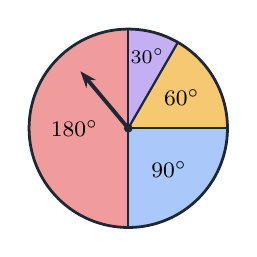
\begin{tikzpicture}[scale=1.05]
\fill[AnsRed!45] (0,0)--(90:1.2) arc (90:270:1.2)--cycle;
\fill[tmBlue!45] (0,0)--(270:1.2) arc (270:360:1.2)--cycle;
\fill[StarGold!70] (0,0)--(0:1.2) arc (0:60:1.2)--cycle;
\fill[tmPurple!45] (0,0)--(60:1.2) arc (60:90:1.2)--cycle;
\draw[Ink,line width=1pt] (0,0) circle (1.2);
\foreach \a in {90,270,0,60}{\draw[Ink,line width=0.8pt] (0,0)--(\a:1.2);}
\node[font=\footnotesize] at (180:0.65){$180^\circ$};
\node[font=\footnotesize] at (315:0.7){$90^\circ$};
\node[font=\footnotesize] at (30:0.75){$60^\circ$};
\node[font=\scriptsize] at (75:0.9){$30^\circ$};
\draw[-{Stealth[length=6pt]},line width=1.4pt,Ink] (0,0)--(130:0.9);\fill[Ink] (0,0) circle (1.5pt);
\end{tikzpicture}
\end{minipage}
\end{probbox}
\probsol{
\textbf{Phân tích đề.} Các ô có kích thước \emph{khác nhau}, nên bốn ô \emph{không} đồng khả năng. Ta không thể dùng ``$1$ ô trên $4$ ô''. Thay vào đó, khả năng kim dừng ở một ô tỉ lệ với độ lớn của ô, tức là với góc ở tâm của ô.
\begin{recallbox}Với bánh xe có các ô không bằng nhau: $P(\text{ô})=\dfrac{\text{góc ở tâm của ô}}{360^\circ}$. Cả vòng tròn có góc $360^\circ$.\end{recallbox}
\step{1}{Kiểm tra số liệu}
$180^\circ+90^\circ+60^\circ+30^\circ=360^\circ$ -- đúng bằng một vòng tròn \checkmark.
\step{2}{Câu a}
$P(\text{xanh})=\dfrac{90}{360}=\dfrac14$.

\emph{Cách nghĩ khác:} ta có thể chia bánh xe thành $12$ ô nhỏ bằng nhau, mỗi ô $30^\circ$. Khi đó đỏ chiếm $6$ ô nhỏ, xanh $3$ ô, vàng $2$ ô, tím $1$ ô; $12$ ô nhỏ này đồng khả năng. $P(\text{xanh})=\dfrac{3}{12}=\dfrac14$ \checkmark.
\step{3}{Câu b}
Ô vàng và ô tím không chồng lên nhau, nên góc tổng là $60^\circ+30^\circ=90^\circ$.
$P(\text{vàng hoặc tím})=\dfrac{90}{360}=\dfrac14$ (hoặc $\dfrac{2+1}{12}=\dfrac{3}{12}=\dfrac14$).
\step{4}{Câu c}
Hùng nói \textbf{sai}. Công thức ``thuận lợi chia tất cả'' chỉ dùng được khi các kết quả \emph{đồng khả năng}. Ở đây bốn màu không đồng khả năng: ô đỏ chiếm nửa bánh xe nên $P(\text{đỏ})=\dfrac{180}{360}=\dfrac12$, còn $P(\text{tím})=\dfrac{30}{360}=\dfrac{1}{12}$ -- khác xa nhau.
\verify{$P(\text{đỏ})+P(\text{xanh})+P(\text{vàng})+P(\text{tím})=\dfrac{6}{12}+\dfrac{3}{12}+\dfrac{2}{12}+\dfrac{1}{12}=1$ \checkmark.}
\begin{parentbox}Có thể cắt một đĩa giấy thành $12$ ``miếng bánh'' bằng nhau rồi tô màu như đề bài. Trẻ đếm số miếng của mỗi màu sẽ hiểu ngay vì sao ô to thì xác suất lớn.\end{parentbox}
\ans{a) $\dfrac14$;\quad b) $\dfrac14$;\quad c) Sai, vì các ô không bằng nhau (ví dụ $P(\text{đỏ})=\dfrac12$, $P(\text{tím})=\dfrac1{12}$).}
}

% ---------------------------------------------------------------- Bài 33
\begin{probbox}{33}{\relax}
Căng tin trường có thực đơn bữa trưa: món chính chọn một trong $3$ món (cơm gà, phở, bún chả); đồ uống chọn một trong $2$ loại (trà đá, nước cam); tráng miệng chọn một trong $2$ món (chè, sữa chua). Mỗi suất ăn gồm một món chính, một đồ uống và một món tráng miệng.
\begin{enumerate}[label=\alph*),leftmargin=1.5em,itemsep=0pt,topsep=2pt]
\item Có bao nhiêu suất ăn khác nhau?
\item Bạn Lan được phát ngẫu nhiên một suất ăn. Tính xác suất suất ăn đó có phở.
\item Tính xác suất suất ăn của Lan có cả phở và nước cam.
\end{enumerate}
\end{probbox}
\probsol{
\textbf{Phân tích đề.} Mỗi suất ăn được tạo bởi ba bước chọn liên tiếp: món chính, đồ uống, tráng miệng. Được ``phát ngẫu nhiên'' nghĩa là mọi suất ăn khác nhau đều đồng khả năng.
\step{1}{Câu a -- quy tắc nhân}
\begin{recallbox}Quy tắc nhân: một việc gồm nhiều bước, bước 1 có $m$ cách, bước 2 có $n$ cách, bước 3 có $p$ cách thì có $m\times n\times p$ cách.\end{recallbox}
Số suất ăn: $3\times2\times2=12$.
\begin{center}\begin{tikzpicture}[grow'=right,level distance=2.6cm,font=\sffamily\footnotesize,
  every node/.style={draw=tmBlue,fill=tmBlue!8,rounded corners=2pt,inner sep=2pt},
  level 1/.style={sibling distance=2.4cm},level 2/.style={sibling distance=1.2cm},level 3/.style={sibling distance=0.6cm},
  edge from parent/.style={draw=Ink!60}]
\node[fill=Ink!10,draw=Ink]{Suất}
  child{node{cơm gà} child{node{trà đá} child{node{chè}} child{node{sữa chua}}} child{node{nước cam} child{node{chè}} child{node{sữa chua}}}}
  child{node[fill=tmOrange!25,draw=tmOrange]{phở} child{node{trà đá} child{node{chè}} child{node{sữa chua}}} child{node[fill=tmOrange!25,draw=tmOrange]{nước cam} child{node[fill=tmOrange!25,draw=tmOrange]{chè}} child{node[fill=tmOrange!25,draw=tmOrange]{sữa chua}}}}
  child{node{bún chả} child{node{trà đá} child{node{chè}} child{node{sữa chua}}} child{node{nước cam} child{node{chè}} child{node{sữa chua}}}};
\end{tikzpicture}\end{center}
Sơ đồ cây có $3$ nhánh lớn, mỗi nhánh lớn tỏa $2$ nhánh, mỗi nhánh đó lại tỏa $2$ nhánh: $12$ ngọn, đúng $12$ suất ăn.
\step{2}{Câu b}
Các suất có phở: món chính cố định là phở, đồ uống $2$ cách, tráng miệng $2$ cách: $1\times2\times2=4$ suất (nhánh giữa của sơ đồ cây).
$P(\text{có phở})=\dfrac{4}{12}=\dfrac13$.
\begin{tipbox}Cũng có thể nghĩ nhanh: món chính được chọn ngẫu nhiên trong $3$ món, mỗi món xuất hiện trong số suất ăn như nhau, nên $P(\text{phở})=\dfrac13$. Đồ uống và tráng miệng không ảnh hưởng.\end{tipbox}
\step{3}{Câu c}
Món chính là phở, đồ uống là nước cam, chỉ còn chọn tráng miệng: $1\times1\times2=2$ suất (tô cam trên sơ đồ).
$P(\text{phở và nước cam})=\dfrac{2}{12}=\dfrac16$.
\verify{Liệt kê: (phở, nước cam, chè) và (phở, nước cam, sữa chua) -- đúng $2$ suất \checkmark.}
\ans{a) $12$ suất;\quad b) $\dfrac13$;\quad c) $\dfrac16$.}
}

% ---------------------------------------------------------------- Bài 34
\begin{probbox}{34}{\relax}
Một hội trường có $20$ hàng ghế. Hàng thứ nhất có $12$ ghế, và mỗi hàng phía sau có nhiều hơn hàng ngay trước nó $2$ ghế.
\begin{enumerate}[label=\alph*),leftmargin=1.5em,itemsep=0pt,topsep=2pt]
\item Hàng thứ $20$ có bao nhiêu ghế?
\item Hàng thứ mấy có đúng $30$ ghế?
\item Hội trường có tất cả bao nhiêu ghế?
\end{enumerate}
\end{probbox}
\probsol{
\textbf{Phân tích đề.} Số ghế các hàng là $12;14;16;\dots$ -- một \emph{dãy cách đều} với khoảng cách $d=2$. Ta cần: số hạng thứ $20$, vị trí của số $30$ và tổng của $20$ số hạng.
\step{1}{Câu a -- tìm quy luật}
\begin{center}
\begin{tabular}{|c|c|c|c|c|c|}\hline
Hàng & $1$ & $2$ & $3$ & $4$ & $k$\\ \hline
Số ghế & $12$ & $12+2$ & $12+2\times2$ & $12+3\times2$ & $12+(k-1)\times2$\\ \hline
\end{tabular}
\end{center}
Từ hàng $1$ đến hàng $k$ có $k-1$ ``bước nhảy'', mỗi bước thêm $2$ ghế. Hàng $20$: $12+19\times2=12+38=50$ ghế.
\begin{warnbox}Không phải $12+20\times2=52$: từ hàng $1$ đến hàng $20$ chỉ có $19$ lần tăng (lỗi ``lệch một'').\end{warnbox}
\step{2}{Câu b}
Cần $12+(k-1)\times2=30$, tức $(k-1)\times2=18$, $k-1=9$, $k=10$. Hàng thứ $10$ có $30$ ghế.
\step{3}{Câu c -- tổng dãy cách đều}
\begin{recallbox}Tổng dãy cách đều $=\dfrac{(\text{số đầu}+\text{số cuối})\times\text{số số hạng}}{2}$ (cách ghép cặp của Gauss).\end{recallbox}
Tổng số ghế: $\dfrac{(12+50)\times20}{2}=\dfrac{62\times20}{2}=620$ ghế.
\begin{proofbox}Ghép hàng $1$ với hàng $20$: $12+50=62$; hàng $2$ với hàng $19$: $14+48=62$; \ldots; hàng $10$ với hàng $11$: $30+32=62$. Có $10$ cặp, mỗi cặp $62$ ghế, nên tổng là $10\times62=620$.\end{proofbox}
\verify{Cách khác: nếu mọi hàng đều có $12$ ghế thì có $20\times12=240$ ghế; phần ``thêm'' là $0+2+4+\dots+38=2\times(0+1+\dots+19)=2\times190=380$; tổng $240+380=620$ \checkmark.}
\ans{a) $50$ ghế;\quad b) hàng thứ $10$;\quad c) $620$ ghế.}
}

% ---------------------------------------------------------------- Bài 35
\begin{probbox}{35}{\stars{1}}
Một hộp chỉ chứa bi đỏ và bi xanh. Lấy ngẫu nhiên một viên thì xác suất được bi đỏ là $\dfrac35$. Nếu bỏ thêm vào hộp $5$ viên bi xanh thì xác suất lấy được bi đỏ chỉ còn $\dfrac12$. Hỏi lúc đầu trong hộp có bao nhiêu bi đỏ, bao nhiêu bi xanh?
\end{probbox}
\probsol{
\textbf{Phân tích đề.} Ta chưa biết tổng số bi, chỉ biết \emph{tỉ lệ}. Thêm bi xanh thì số bi đỏ không đổi. Hãy dịch hai xác suất sang ngôn ngữ ``phần bằng nhau'' (sơ đồ đoạn thẳng).
\step{1}{Dịch điều kiện thứ nhất}
$P(\text{đỏ})=\dfrac35$: nếu chia số bi thành $5$ phần bằng nhau thì bi đỏ chiếm $3$ phần, bi xanh chiếm $5-3=2$ phần.
\step{2}{Dịch điều kiện thứ hai}
Sau khi thêm $5$ bi xanh, $P(\text{đỏ})=\dfrac12$: bi đỏ chiếm đúng một nửa, tức là \emph{số bi đỏ bằng số bi xanh}.
\step{3}{Vẽ sơ đồ và so sánh}
\begin{figC}
\rowlab{-0.15}{0}{Đỏ}
\blk{0}{1.5}{0}{0.55}{AnsRed}{1 phần}\blk{1.5}{3}{0}{0.55}{AnsRed}{1 phần}\blk{3}{4.5}{0}{0.55}{AnsRed}{1 phần}
\rowlab{-0.15}{-0.8}{Xanh}
\blk{0}{1.5}{-0.8}{0.55}{tmBlue}{1 phần}\blk{1.5}{3}{-0.8}{0.55}{tmBlue}{1 phần}\blk{3}{4.5}{-0.8}{0.55}{tmTeal}{thêm 5}
\brcdn{3}{4.5}{-1.25}{$1$ phần $=5$ viên}
\end{figC}
Bi đỏ: $3$ phần. Bi xanh sau khi thêm: $2$ phần $+\ 5$ viên. Hai số này bằng nhau, nên $5$ viên chính là $3-2=1$ phần.
\step{4}{Tính số bi lúc đầu}
$1$ phần $=5$ viên. Bi đỏ: $3\times5=15$ viên. Bi xanh: $2\times5=10$ viên.
\begin{tipbox}\emph{Cách đại số (cho bạn nào thích):} gọi số bi đỏ là $3k$, bi xanh là $2k$. Sau khi thêm: $3k=2k+5$, nên $k=5$.\end{tipbox}
\verify{Lúc đầu: $15$ đỏ, $10$ xanh, $P(\text{đỏ})=\dfrac{15}{25}=\dfrac35$ \checkmark. Thêm $5$ xanh: $15$ đỏ, $15$ xanh, $P(\text{đỏ})=\dfrac{15}{30}=\dfrac12$ \checkmark.}
\begin{warnbox}Đừng giải bằng cách ``trừ xác suất'': $\dfrac35-\dfrac12=\dfrac1{10}$ không cho biết gì trực tiếp về số bi. Xác suất là \emph{tỉ số}, phải quay về số lượng cụ thể.\end{warnbox}
\ans{Lúc đầu có $15$ bi đỏ và $10$ bi xanh.}
}

% ---------------------------------------------------------------- Bài 36
\begin{probbox}{36}{\stars{1}}
Nhắc lại: số đối xứng là số đọc xuôi hay đọc ngược đều như nhau (ví dụ $3443$, $7007$).
\begin{enumerate}[label=\alph*),leftmargin=1.5em,itemsep=0pt,topsep=2pt]
\item Có bao nhiêu số đối xứng có bốn chữ số?
\item Trong đó có bao nhiêu số chẵn?
\item Chọn ngẫu nhiên một số đối xứng có bốn chữ số. Tính xác suất số đó là số chẵn.
\item Chứng tỏ rằng mọi số đối xứng có bốn chữ số đều chia hết cho $11$.
\end{enumerate}
\end{probbox}
\probsol{
\textbf{Phân tích đề.} Số có bốn chữ số $\overline{abcd}$ là số đối xứng khi đọc ngược $\overline{dcba}$ vẫn là nó: $d=a$ và $c=b$. Vậy số đối xứng có bốn chữ số có dạng $\overline{abba}$, và chỉ có \emph{hai} chữ số được chọn tự do: $a$ và $b$.
\step{1}{Câu a}
\begin{recallbox}Quy tắc nhân; chữ số đầu tiên của một số không được là $0$.\end{recallbox}
\countboxes{chữ số a/9/từ 1 đến 9/tmBlue,chữ số b/10/từ 0 đến 9/tmOrange,thứ ba/1/bằng b/tmGreen,thứ tư/1/bằng a/tmGreen}{90}
$a$: $9$ cách ($1$ đến $9$); $b$: $10$ cách; hai chữ số sau bị ép bằng $b$ và $a$. Có $9\times10=90$ số.
\step{2}{Câu b}
Số chẵn khi chữ số hàng đơn vị chẵn. Chữ số hàng đơn vị chính là $a$, nên $a$ phải chẵn \emph{và} khác $0$: $a\in\{2;4;6;8\}$ -- $4$ cách. $b$ vẫn có $10$ cách. Có $4\times10=40$ số chẵn.
\begin{warnbox}Chữ số $0$ là chữ số chẵn, nhưng $a=0$ bị loại vì $a$ còn là chữ số đầu tiên. Vì vậy chỉ có $4$ chứ không phải $5$ lựa chọn cho $a$.\end{warnbox}
\step{3}{Câu c}
$P(\text{chẵn})=\dfrac{40}{90}=\dfrac49$.
\step{4}{Câu d -- chứng minh}
\begin{proofbox}Viết số $\overline{abba}$ theo giá trị các hàng:
$\overline{abba}=1000a+100b+10b+a=1001a+110b$.
Mà $1001=11\times91$ và $110=11\times10$, nên
$\overline{abba}=11\times91\times a+11\times10\times b=11\times(91a+10b)$,
là một số chia hết cho $11$.\end{proofbox}
\verify{Ví dụ: $3443=11\times313$; $7007=11\times637$; $1221=11\times111$ \checkmark. Kiểm tra đếm: các số đối xứng bắt đầu bằng $1$ là $1001;1111;\dots;1991$ -- đúng $10$ số; chín chữ số đầu cho $90$ số \checkmark.}
\ans{a) $90$;\quad b) $40$;\quad c) $\dfrac49$;\quad d) $\overline{abba}=11\times(91a+10b)$.}
}

% ---------------------------------------------------------------- Bài 37
\begin{probbox}{37}{\stars{1}}
Từ bốn chữ số $0;1;2;3$, lập các số có bốn chữ số đôi một khác nhau (mỗi chữ số dùng đúng một lần).
\begin{enumerate}[label=\alph*),leftmargin=1.5em,itemsep=0pt,topsep=2pt]
\item Lập được bao nhiêu số như vậy?
\item Có bao nhiêu số chẵn trong các số đó?
\item Chọn ngẫu nhiên một số trong các số ở câu a). Tính xác suất số đó là số chẵn.
\end{enumerate}
\end{probbox}
\probsol{
\textbf{Phân tích đề.} Mỗi số là một cách xếp bốn chữ số $0;1;2;3$ vào bốn hàng (nghìn, trăm, chục, đơn vị), với điều kiện chữ số hàng nghìn khác $0$.
\step{1}{Câu a -- chọn vị trí có điều kiện trước}
\begin{recallbox}Quy tắc nhân. Vị trí nào có điều kiện thì chọn trước.\end{recallbox}
\countboxes{hàng nghìn/3/1 2 hoặc 3/tmBlue,hàng trăm/3/kể cả 0/tmOrange,hàng chục/2/còn lại/tmGreen,đơn vị/1/còn lại/tmPurple}{18}
Hàng nghìn: $3$ cách ($1$, $2$ hoặc $3$). Hàng trăm: còn $3$ chữ số (bây giờ được dùng $0$): $3$ cách. Hàng chục: $2$ cách. Hàng đơn vị: $1$ cách. Có $3\times3\times2\times1=18$ số.
\begin{warnbox}Nếu quên điều kiện ``hàng nghìn khác $0$'' sẽ được $4\times3\times2\times1=24$ -- trong đó có $6$ ``số'' bắt đầu bằng $0$ như $0123$, thực chất chỉ là số có ba chữ số.\end{warnbox}
\step{2}{Câu b -- chia trường hợp theo chữ số hàng đơn vị}
Số chẵn thì hàng đơn vị là $0$ hoặc $2$. Hai trường hợp này khác nhau ở chỗ: chữ số $0$ có ảnh hưởng đến hàng nghìn.
\begin{itemize}[leftmargin=1.2em,itemsep=1pt,topsep=1pt]
\item \textbf{Trường hợp 1: hàng đơn vị là $0$.} Ba chữ số $1;2;3$ xếp tự do vào ba hàng còn lại (không còn lo chữ số $0$ ở đầu): $3\times2\times1=6$ số.
\item \textbf{Trường hợp 2: hàng đơn vị là $2$.} Còn $0;1;3$. Hàng nghìn khác $0$: $2$ cách ($1$ hoặc $3$); hàng trăm: $2$ cách; hàng chục: $1$ cách. Có $2\times2\times1=4$ số.
\end{itemize}
\begin{recallbox}Quy tắc cộng: các trường hợp tách rời nhau thì cộng số cách của từng trường hợp.\end{recallbox}
Số các số chẵn: $6+4=10$.
\step{3}{Câu c}
$P(\text{chẵn})=\dfrac{10}{18}=\dfrac59$.
\verify{Liệt kê các số chẵn. TH1: $1230;1320;2130;2310;3120;3210$ ($6$ số). TH2: $1032;1302;3012;3102$ ($4$ số). Tổng $10$ \checkmark. Số lẻ (tận cùng $1$ hoặc $3$): mỗi trường hợp giống TH2, có $4$ số, tổng $8$; và $10+8=18$ \checkmark.}
\ans{a) $18$ số;\quad b) $10$ số chẵn;\quad c) $\dfrac59$.}
}

% ---------------------------------------------------------------- Bài 38
\begin{probbox}{38}{\stars{1}}
\begin{minipage}[t]{0.62\linewidth}\vspace{0pt}
Hình bên là một lưới hình chữ nhật gồm $2$ hàng, $3$ cột ô vuông.
\begin{enumerate}[label=\alph*),leftmargin=1.5em,itemsep=0pt,topsep=2pt]
\item Trong hình có tất cả bao nhiêu hình chữ nhật (kể cả hình vuông)?
\item Có bao nhiêu hình vuông?
\item Chọn ngẫu nhiên một hình chữ nhật trong số đó. Tính xác suất nó là hình vuông.
\end{enumerate}
\end{minipage}\hfill
\begin{minipage}[t]{0.34\linewidth}\vspace{0pt}
\centering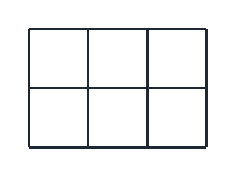
\begin{tikzpicture}[scale=0.75]
\foreach \x in {0,1,2,3}{\draw[Ink,line width=1pt] (\x,0)--(\x,2);}
\foreach \y in {0,1,2}{\draw[Ink,line width=1pt] (0,\y)--(3,\y);}
\end{tikzpicture}
\end{minipage}
\end{probbox}
\probsol{
\textbf{Phân tích đề.} Đây là một lưới kẻ suốt, nên dùng được mẹo ``chọn hai đường''. Ta cũng sẽ đếm theo kích thước để kiểm tra lại.
\step{1}{Câu a -- chọn hai đường ngang và hai đường dọc}
\begin{recallbox}Một hình chữ nhật trong lưới được xác định bởi $2$ đường ngang và $2$ đường dọc. Số cách chọn $2$ đường trong $n$ đường là $\dfrac{n\times(n-1)}{2}$.\end{recallbox}
Lưới có $3$ đường ngang và $4$ đường dọc.
\begin{itemize}[leftmargin=1.2em,itemsep=0pt,topsep=1pt]
\item Chọn $2$ đường ngang: $\dfrac{3\times2}{2}=3$ cách.
\item Chọn $2$ đường dọc: $\dfrac{4\times3}{2}=6$ cách.
\end{itemize}
Theo quy tắc nhân: $3\times6=18$ hình chữ nhật.
\step{2}{Kiểm tra bằng bảng kích thước}
Kí hiệu ``cao $\times$ rộng'' (theo số ô). Một hình rộng $w$ ô có $4-w$ vị trí theo chiều ngang; cao $h$ ô có $3-h$ vị trí theo chiều dọc.
\begin{center}
\begin{tabular}{|c|c|c|c|c|c|c|c|}\hline
Kích thước & $1\times1$ & $1\times2$ & $1\times3$ & $2\times1$ & $2\times2$ & $2\times3$ & Tổng\\ \hline
Số hình & $2\times3=6$ & $2\times2=4$ & $2\times1=2$ & $1\times3=3$ & $1\times2=2$ & $1\times1=1$ & $18$\\ \hline
\end{tabular}
\end{center}
Hai cách cho cùng kết quả $18$ \checkmark.
\step{3}{Câu b}
Hình vuông là các hình $1\times1$ và $2\times2$: $6+2=8$ hình vuông.
\begin{warnbox}Không có hình vuông $3\times3$ vì lưới chỉ cao $2$ ô. Và đừng quên hai hình vuông $2\times2$ (bên trái và bên phải, chồng lên nhau ở cột giữa).\end{warnbox}
\step{4}{Câu c}
$P(\text{hình vuông})=\dfrac{8}{18}=\dfrac49$.
\ans{a) $18$;\quad b) $8$;\quad c) $\dfrac49$.}
}

% ---------------------------------------------------------------- Bài 39
\begin{probbox}{39}{\stars{1}}
Bốn bạn An, Bình, Chi, Dũng được xếp ngẫu nhiên vào bốn chiếc ghế xếp thành một hàng ngang.
\begin{enumerate}[label=\alph*),leftmargin=1.5em,itemsep=0pt,topsep=2pt]
\item Có bao nhiêu cách xếp chỗ?
\item Tính xác suất An và Bình ngồi cạnh nhau.
\item Tính xác suất An và Bình ngồi ở hai đầu hàng.
\end{enumerate}
\end{probbox}
\probsol{
\textbf{Phân tích đề.} ``Xếp ngẫu nhiên'' nghĩa là mọi cách xếp đều đồng khả năng. Ta đếm tổng số cách xếp, rồi đếm số cách thuận lợi cho từng biến cố. Đánh số ghế $1;2;3;4$ từ trái sang phải.
\step{1}{Câu a}
\begin{recallbox}Xếp $n$ người vào $n$ ghế: $n\times(n-1)\times\dots\times2\times1$ cách (quy tắc nhân, mỗi ghế sau còn ít hơn một người để chọn).\end{recallbox}
Ghế $1$: $4$ cách chọn người; ghế $2$: $3$ cách; ghế $3$: $2$ cách; ghế $4$: $1$ cách. Có $4\times3\times2\times1=24$ cách.
\step{2}{Câu b -- xem An và Bình là một ``khối''}
\begin{figC}
\draw[tmOrange,line width=1.2pt,rounded corners=4pt,fill=tmOrange!12] (0,0) rectangle (2.4,0.7);
\node[font=\bfseries] at (0.6,0.35){An};\node[font=\bfseries] at (1.8,0.35){Bình};
\draw[tmBlue,line width=1pt,rounded corners=3pt,fill=tmBlue!10] (2.7,0) rectangle (3.9,0.7);\node[font=\bfseries] at (3.3,0.35){Chi};
\draw[tmGreen,line width=1pt,rounded corners=3pt,fill=tmGreen!10] (4.2,0) rectangle (5.4,0.7);\node[font=\bfseries] at (4.8,0.35){Dũng};
\node[font=\footnotesize,text=tmOrange!80!black] at (1.2,-0.3){một khối, chiếm $2$ ghế liền nhau};
\end{figC}
\begin{itemize}[leftmargin=1.2em,itemsep=1pt,topsep=1pt]
\item Vị trí của khối (An, Bình): chiếm ghế $1$--$2$, $2$--$3$ hoặc $3$--$4$: $3$ cách.
\item Trong khối, An bên trái hoặc Bình bên trái: $2$ cách.
\item Chi và Dũng xếp vào $2$ ghế còn lại: $2\times1=2$ cách.
\end{itemize}
Số cách thuận lợi: $3\times2\times2=12$. Vậy $P(\text{cạnh nhau})=\dfrac{12}{24}=\dfrac12$.
\begin{warnbox}Đừng quên nhân $2$ cho việc đổi chỗ An và Bình bên trong khối: ``An--Bình'' và ``Bình--An'' là hai cách xếp khác nhau.\end{warnbox}
\step{3}{Câu c}
An và Bình ở ghế $1$ và ghế $4$: An ở ghế $1$, Bình ở ghế $4$ hoặc ngược lại -- $2$ cách. Chi và Dũng vào ghế $2$, $3$: $2$ cách. Số cách thuận lợi: $2\times2=4$.
$P(\text{hai đầu})=\dfrac{4}{24}=\dfrac16$.
\verify{Câu b, đếm theo cách khác: An ngồi ở đầu hàng (ghế $1$ hoặc $4$, $2$ khả năng) thì chỉ có $1$ ghế cạnh An; An ngồi ở giữa (ghế $2$ hoặc $3$) thì có $2$ ghế cạnh An. Số cặp ghế (An, Bình) cạnh nhau: $2\times1+2\times2=6$; nhân với $2$ cách xếp Chi, Dũng: $12$ \checkmark.}
\begin{parentbox}Với bài $4$ người, có thể cho trẻ dùng $4$ tấm thẻ ghi tên và thật sự xếp hết $24$ cách theo thứ tự (bắt đầu bằng An, rồi bắt đầu bằng Bình\ldots). Liệt kê một lần giúp trẻ tin vào quy tắc nhân.\end{parentbox}
\ans{a) $24$ cách;\quad b) $\dfrac12$;\quad c) $\dfrac16$.}
}

% ---------------------------------------------------------------- Bài 40
\begin{probbox}{40}{\stars{2}}
Một hộp có $4$ viên bi đỏ và $6$ viên bi xanh có cùng kích thước. Bạn Hoa lấy ngẫu nhiên một viên bi, \emph{không trả lại}, rồi lấy ngẫu nhiên tiếp viên thứ hai.
\begin{enumerate}[label=\alph*),leftmargin=1.5em,itemsep=0pt,topsep=2pt]
\item Tính xác suất cả hai viên đều là bi đỏ.
\item Tính xác suất hai viên bi cùng màu.
\item Tính xác suất hai viên bi khác màu.
\end{enumerate}
\end{probbox}
\probsol{
\textbf{Phân tích đề.} Hoa lấy \emph{lần lượt} hai viên và không trả lại. Hãy tưởng tượng các viên bi được đánh số $1$ đến $10$ (bi $1$--$4$ đỏ, bi $5$--$10$ xanh). Mỗi \emph{cặp có thứ tự} (viên thứ nhất, viên thứ hai) là một kết quả, và các kết quả này đồng khả năng.
\step{1}{Đếm tất cả các kết quả}
\begin{recallbox}Quy tắc nhân: lần $1$ có $10$ cách; với mỗi cách đó, lần $2$ còn $9$ viên nên có $9$ cách.\end{recallbox}
Số kết quả: $10\times9=90$ cặp có thứ tự.
\step{2}{Câu a -- cả hai đỏ}
Lần $1$ lấy bi đỏ: $4$ cách. Khi đó còn $3$ bi đỏ, lần $2$ lấy bi đỏ: $3$ cách. Số kết quả thuận lợi: $4\times3=12$.
$P(\text{đỏ, đỏ})=\dfrac{12}{90}=\dfrac{2}{15}$.
\step{3}{Sơ đồ cây có ghi số cách}
\begin{center}\begin{tikzpicture}[grow'=right,level distance=3.1cm,font=\sffamily\footnotesize,
  every node/.style={draw=Ink!60,rounded corners=2pt,inner sep=2.5pt,fill=white},
  level 1/.style={sibling distance=2.2cm},level 2/.style={sibling distance=1.1cm},
  edge from parent/.style={draw=Ink!60}]
\node[fill=Ink!10]{Bắt đầu}
  child{node[fill=AnsRed!15,draw=AnsRed]{Đỏ: $4$ cách}
     child{node[fill=AnsRed!15,draw=AnsRed]{Đỏ: $3$ cách $\Rightarrow 4\times3=12$}}
     child{node[fill=tmBlue!15,draw=tmBlue]{Xanh: $6$ cách $\Rightarrow 4\times6=24$}}}
  child{node[fill=tmBlue!15,draw=tmBlue]{Xanh: $6$ cách}
     child{node[fill=AnsRed!15,draw=AnsRed]{Đỏ: $4$ cách $\Rightarrow 6\times4=24$}}
     child{node[fill=tmBlue!15,draw=tmBlue]{Xanh: $5$ cách $\Rightarrow 6\times5=30$}}};
\end{tikzpicture}\end{center}
Kiểm tra: $12+24+24+30=90$ \checkmark{} -- bốn nhánh phủ hết mọi kết quả.
\step{4}{Câu b -- cùng màu}
Cùng màu gồm hai trường hợp tách rời: (đỏ, đỏ) có $12$ kết quả và (xanh, xanh) có $30$ kết quả.
\begin{recallbox}Quy tắc cộng cho các trường hợp không chồng lên nhau.\end{recallbox}
Số kết quả thuận lợi: $12+30=42$. $P(\text{cùng màu})=\dfrac{42}{90}=\dfrac{7}{15}$.
\step{5}{Câu c -- biến cố đối}
``Khác màu'' là biến cố đối của ``cùng màu'': $P(\text{khác màu})=1-\dfrac{7}{15}=\dfrac{8}{15}$.
\verify{Đếm trực tiếp: (đỏ, xanh) $24$ và (xanh, đỏ) $24$, tổng $48$; $\dfrac{48}{90}=\dfrac{8}{15}$ \checkmark.}
\begin{warnbox}Lỗi hay gặp nhất: coi như lần hai vẫn còn đủ $10$ viên, tính $\dfrac{4}{10}\times\dfrac{4}{10}$ hoặc đếm $4\times4$ cặp đỏ. Vì \emph{không trả lại}, lần hai chỉ còn $9$ viên và chỉ còn $3$ viên đỏ.\end{warnbox}
\begin{tipbox}Có thể đếm không theo thứ tự: số cách chọn $2$ viên trong $10$ viên là $\dfrac{10\times9}{2}=45$, số cách chọn $2$ viên đỏ trong $4$ viên là $\dfrac{4\times3}{2}=6$, nên $P(\text{đỏ, đỏ})=\dfrac{6}{45}=\dfrac{2}{15}$ -- cùng kết quả. Điều quan trọng là tử số và mẫu số phải đếm \emph{cùng một kiểu} (cùng có thứ tự hoặc cùng không thứ tự).\end{tipbox}
\ans{a) $\dfrac{2}{15}$;\quad b) $\dfrac{7}{15}$;\quad c) $\dfrac{8}{15}$.}
}

% ---------------- part d ----------------
% ================= Topic 3 (VI) -- part d: problems 41--50 (nâng cao) =================
\begin{probbox}{41}{\stars{1}}
Trên một lưới điểm vuông, bạn Lan đứng ở điểm $A$. Lan tung một đồng xu cân đối $6$ lần; mỗi lần ra mặt sấp thì Lan đi
\emph{lên} một điểm, ra mặt ngửa thì Lan đi \emph{sang phải} một điểm (như bài 16). Các điểm $M$, $N$, $B$ được đánh dấu
trên hình.
\begin{figC}\begin{scope}[scale=0.85]
  \foreach \x in {0,...,3}{\foreach \y in {0,...,3}{\fill[Navy] (\x,\y) circle (2.4pt);}}
  \fill[tmOrange] (0,0) circle (3.4pt);\node[below left] at (0,0) {$A$};
  \fill[tmGreen!80!black] (1,1) circle (3.4pt);\node[above left] at (1,1) {$M$};
  \fill[AnsRed] (2,1) circle (3.4pt);\node[below right] at (2,1) {$N$};
  \fill[tmPurple] (3,3) circle (3.4pt);\node[above right] at (3,3) {$B$};
\end{scope}\end{figC}
\begin{enumerate}[label=\alph*),leftmargin=1.6em,itemsep=1pt,topsep=2pt]
\item Tính xác suất để sau $6$ lần tung, Lan dừng ở điểm $B$.
\item Tính xác suất để Lan đi qua điểm $M$ \emph{và} dừng ở $B$.
\item Tính xác suất để Lan dừng ở $B$ mà \emph{không} đi qua điểm $N$.
\end{enumerate}
\end{probbox}
\probsol{
\textbf{Phân tích đề.} Mỗi dãy $6$ lần tung là một dãy gồm $6$ kí hiệu $\uparrow$ (lên) hoặc $\rightarrow$ (sang phải).
Có $2^6=2\times2\times2\times2\times2\times2=64$ dãy, đồng khả năng. Mỗi dãy là một \emph{đường đi} trên lưới.
Ta đánh dấu vị trí bằng cặp (số bước sang phải, số bước lên): $A=(0,0)$, $M=(1,1)$, $N=(2,1)$, $B=(3,3)$.

\step{1}{Đếm số đường đi từ $A$ tới mỗi điểm (câu a)}
\begin{recallbox}Một điểm chỉ có thể tới được từ điểm ngay bên trái hoặc ngay bên dưới nó. Vì vậy:
số đường tới một điểm $=$ số đường tới điểm bên trái $+$ số đường tới điểm bên dưới (quy tắc cộng).\end{recallbox}
Ghi số đường đi vào từng điểm, bắt đầu từ $A$ (ghi $1$); hàng dưới cùng và cột trái cùng đều là $1$:
\begin{figC}\begin{scope}[scale=0.85]
  \foreach \x/\y/\n in {0/0/1,1/0/1,2/0/1,3/0/1,0/1/1,1/1/2,2/1/3,3/1/4,0/2/1,1/2/3,2/2/6,3/2/10,0/3/1,1/3/4,2/3/10,3/3/20}{
    \fill[tmBlue!12] (\x,\y) circle (9pt);\node[font=\small\bfseries,text=Navy] at (\x,\y) {\n};}
  \draw[tmPurple,thick] (3,3) circle (10pt);\node[right=9pt,text=tmPurple] at (3,3) {$B$};
\end{scope}\end{figC}
Có $20$ đường đi từ $A$ tới $B$. (Cách khác: đi tới $B$ cần đúng $3$ bước lên trong $6$ bước; số cách chọn $3$ lượt
trong $6$ lượt là $\dfrac{6\times5\times4}{3\times2\times1}=20$.)
\[P(a)=\frac{20}{64}=\frac{5}{16}.\]

\step{2}{Câu b: đi qua $M$ rồi tới $B$ -- quy tắc nhân}
Một đường qua $M$ gồm hai chặng: chặng $A\to M$ ($1$ bước lên, $1$ bước phải) và chặng $M\to B$ ($2$ bước lên, $2$ bước phải).
Chặng $A\to M$ có $2$ cách ($\uparrow\rightarrow$ hoặc $\rightarrow\uparrow$); chặng $M\to B$ có $6$ cách (giống bài 16:
chọn $2$ lượt lên trong $4$ lượt). Mỗi cách đi chặng đầu ghép với mỗi cách đi chặng sau cho một đường khác nhau:
$2\times6=12$ đường.
\[P(b)=\frac{12}{64}=\frac{3}{16}.\]

\step{3}{Câu c: không đi qua $N$ -- dùng phần bù}
Số đường từ $A$ qua $N$ tới $B$: chặng $A\to N$ ($2$ bước phải, $1$ bước lên) có $3$ cách; chặng $N\to B$ ($1$ bước phải,
$2$ bước lên) có $3$ cách; tổng $3\times3=9$ đường. Vậy số đường từ $A$ tới $B$ \emph{không} qua $N$ là $20-9=11$.
\[P(c)=\frac{11}{64}.\]
\begin{proofbox}\emph{Kiểm tra bằng cách ``chặn'' điểm $N$.} Ghi lại số đường đi nhưng đặt số $0$ tại $N$ (coi như không được đi qua).
Hàng $1$: $1,\ 2,\ \mathbf{0},\ 0+1=1$. Hàng $2$: $1,\ 3,\ 3+0=3,\ 3+1=4$. Hàng $3$: $1,\ 4,\ 4+3=7,\ 7+4=11$.
Tại $B$ được $11$, khớp với phần bù.\end{proofbox}
\begin{warnbox}Câu b và c hỏi về xác suất trong \emph{toàn bộ} $64$ dãy tung, không phải trong $20$ đường tới $B$. Nếu chia cho $20$
là trả lời một câu hỏi khác (xác suất có điều kiện, chưa học).\end{warnbox}
\verify{Ở câu a, các điểm cuối có thể là $(6,0),(5,1),\dots,(0,6)$ với số đường $1,6,15,20,15,6,1$; tổng $=64$. Điểm $B=(3,3)$ ứng với số $20$.}
\ans{a) $\dfrac5{16}$;\quad b) $\dfrac3{16}$;\quad c) $\dfrac{11}{64}$}
}

\begin{probbox}{42}{\stars{2}}
Ta xếp các lưới ô vuông bằng que tăm như ở bài 17. Một lưới ``$m\times n$'' có $m$ hàng, mỗi hàng $n$ ô vuông.
\begin{enumerate}[label=\alph*),leftmargin=1.6em,itemsep=1pt,topsep=2pt]
\item Lập công thức tính số que tăm cần dùng cho lưới $m\times n$.
\item Một lưới hình vuông $k\times k$ dùng hết đúng $760$ que tăm. Tìm $k$.
\item Bạn Nam có đúng $2026$ que tăm và muốn xếp một lưới $m\times n$ (với $1\le m\le n$) dùng \emph{hết} số que này.
Tìm tất cả các lưới Nam có thể xếp.
\end{enumerate}
\end{probbox}
\probsol{
\textbf{Phân tích đề.} Giống bài 17, ta đếm riêng que nằm ngang và que thẳng đứng. Câu c dẫn tới một phương trình với hai ẩn
là số tự nhiên; mẹo ``nhân $2$ rồi cộng $1$'' giúp biến nó thành bài toán tìm ước.

\step{1}{Câu a: công thức}
Lưới $m\times n$ có $m+1$ đường kẻ ngang, mỗi đường $n$ que: $(m+1)\times n$ que nằm ngang. Có $n+1$ đường kẻ dọc, mỗi đường
$m$ que: $(n+1)\times m$ que thẳng đứng. Tổng:
\[T=(m+1)n+(n+1)m=mn+n+mn+m=2mn+m+n.\]
Thử lại với lưới $1\times10$: $2\times1\times10+1+10=31$. Đúng như bài 17.

\step{2}{Câu b: lưới vuông $k\times k$}
Thay $m=n=k$: $T=2k^2+2k=2k(k+1)$. Ta cần $2k(k+1)=760$, tức $k(k+1)=380$.
$k(k+1)$ là tích hai số tự nhiên liên tiếp. Vì $19\times20=380$, nên $k=19$. (Khi $k$ tăng thì $k(k+1)$ tăng, nên chỉ có một
giá trị: $18\times19=342<380<420=20\times21$.)

\step{3}{Câu c: lập phương trình}
Cần tìm các số tự nhiên $1\le m\le n$ với $2mn+m+n=2026$.
\begin{tipbox}Nhân hai vế với $2$ rồi cộng $1$: $4mn+2m+2n+1=4053$. Vế trái phân tích được thành tích:
$(2m+1)(2n+1)=4mn+2m+2n+1$ (nhân phân phối để kiểm tra). Vậy
\[(2m+1)(2n+1)=4053.\]\end{tipbox}

\step{4}{Phân tích $4053$ ra thừa số nguyên tố}
$4053$ có tổng chữ số $4+0+5+3=12$ chia hết cho $3$: $4053=3\times1351$. Tiếp theo $1351=7\times193$.
Số $193$ là số nguyên tố: nó không chia hết cho $2,3,5,7,11,13$, và $13\times13=169<193<196=14\times14$, nên không cần thử thêm.
\begin{recallbox}Để kiểm tra $N$ có là số nguyên tố không, chỉ cần thử chia cho các số nguyên tố $p$ với $p\times p\le N$.\end{recallbox}
Vậy $4053=3\times7\times193$. Các ước của $4053$ là: $1,\ 3,\ 7,\ 21,\ 193,\ 579,\ 1351,\ 4053$.

\step{5}{Tìm các cặp $(m,n)$}
Vì $m\ge1$ nên $2m+1\ge3$; vì $m\le n$ nên $2m+1\le2n+1$. Các cách viết $4053$ thành tích hai ước thỏa mãn:
\begin{center}\begin{tabular}{|c|c|c|c|c|}\hline
$2m+1$ & $2n+1$ & $m$ & $n$ & Thử lại $2mn+m+n$\\\hline
$3$ & $1351$ & $1$ & $675$ & $1350+1+675=2026$\\\hline
$7$ & $579$ & $3$ & $289$ & $1734+3+289=2026$\\\hline
$21$ & $193$ & $10$ & $96$ & $1920+10+96=2026$\\\hline
\end{tabular}\end{center}
(Cặp $1\times4053$ bị loại vì cho $m=0$.)
\begin{warnbox}Thử từng giá trị $m=1,2,3,\dots$ cũng làm được nhưng rất dài, dễ sót. Mẹo nhân $2$ cộng $1$ biến bài toán thành
``tìm ước'' và đảm bảo \emph{không bỏ sót} nghiệm nào.\end{warnbox}
\verify{Ở các giá trị $m$ khác, $2m+1$ không phải là ước của $4053$ nên $n$ không là số tự nhiên. Ví dụ $m=2$: $5(2n+1)=4053$ không
được vì $4053$ không chia hết cho $5$.}
\ans{a) $2mn+m+n$;\quad b) $k=19$;\quad c) ba lưới: $1\times675$, $3\times289$, $10\times96$}
}

\begin{probbox}{43}{\stars{1}}
Gieo cùng lúc ba con xúc xắc cân đối có màu đỏ, xanh và vàng (mỗi con ghi số từ $1$ đến $6$). Tính xác suất của các biến cố:
\begin{enumerate}[label=\alph*),leftmargin=1.6em,itemsep=1pt,topsep=2pt]
\item ba số xuất hiện đôi một khác nhau;
\item số trên con đỏ nhỏ hơn số trên con xanh, và số trên con xanh nhỏ hơn số trên con vàng;
\item có ít nhất một con xúc xắc ra số $6$;
\item số lớn nhất trong ba số xuất hiện bằng đúng $4$.
\end{enumerate}
\end{probbox}
\probsol{
\textbf{Phân tích đề.} Mỗi kết quả là bộ ba (đỏ, xanh, vàng). Theo quy tắc nhân có $6\times6\times6=216$ kết quả đồng khả năng.

\step{1}{Câu a: ba số khác nhau}
Con đỏ: $6$ cách; con xanh khác con đỏ: $5$ cách; con vàng khác hai con kia: $4$ cách. Có $6\times5\times4=120$ kết quả.
\[P(a)=\frac{120}{216}=\frac{5}{9}.\]

\step{2}{Câu b: đỏ $<$ xanh $<$ vàng -- dùng tính đối xứng}
Xét một bộ ba số khác nhau, chẳng hạn $\{2,3,5\}$. Có $3\times2\times1=6$ cách xếp ba số này cho ba con xúc xắc
($235$, $253$, $325$, $352$, $523$, $532$), và \emph{chỉ đúng một} cách là tăng dần ($2<3<5$).
Như vậy $120$ kết quả ở câu a chia thành các nhóm $6$, mỗi nhóm có $1$ kết quả thuận lợi: số kết quả thuận lợi là $120:6=20$.
\[P(b)=\frac{20}{216}=\frac{5}{54}.\]
\begin{recallbox}Số cách xếp $3$ vật khác nhau vào $3$ chỗ là $3\times2\times1=6$.\end{recallbox}

\step{3}{Câu c: ít nhất một số $6$ -- phần bù}
Biến cố đối là ``không con nào ra $6$'': mỗi con chỉ có $5$ kết quả ($1$ đến $5$), tổng $5\times5\times5=125$.
Vậy số kết quả có ít nhất một số $6$ là $216-125=91$.
\[P(c)=\frac{91}{216}.\]
\begin{warnbox}Không được tính ``mỗi con có xác suất $\frac16$ ra số $6$, ba con là $\frac36=\frac12$''. Cách cộng đó đếm trùng các kết quả
có hai hoặc ba số $6$ (như $(6,6,1)$ bị đếm hai lần).\end{warnbox}

\step{4}{Câu d: số lớn nhất bằng đúng $4$}
``Số lớn nhất $\le4$'' nghĩa là cả ba số đều thuộc $\{1,2,3,4\}$: $4\times4\times4=64$ kết quả.
``Số lớn nhất $\le3$'': $3\times3\times3=27$ kết quả. Số lớn nhất bằng đúng $4$ khi nó $\le4$ nhưng không $\le3$:
$64-27=37$ kết quả.
\[P(d)=\frac{37}{216}.\]
\begin{proofbox}Mọi kết quả có số lớn nhất $\le3$ đều nằm trong nhóm có số lớn nhất $\le4$. Bớt đi nhóm nhỏ còn lại đúng các kết
quả mà số lớn nhất không vượt quá $4$ nhưng vượt quá $3$, tức là bằng $4$.\end{proofbox}
\verify{Cách nghĩ của câu d áp dụng cho câu c: số lớn nhất bằng $6$ có $6^3-5^3=216-125=91$ kết quả, khớp. Tổng số kết quả theo
số lớn nhất $1,2,\dots,6$: $1+7+19+37+61+91=216$.}
\ans{a) $\dfrac59$;\quad b) $\dfrac5{54}$;\quad c) $\dfrac{91}{216}$;\quad d) $\dfrac{37}{216}$}
}

\begin{probbox}{44}{\stars{2}}
Người ta làm các con xúc xắc đặc biệt có $6$ mặt, mỗi mặt ghi một số trong các số $1,2,3,4,5,6$ (được phép ghi trùng), sao cho
giống bài 19: xác suất gieo được số chia hết cho $3$ là $\frac12$ và xác suất gieo được số chẵn là $\frac13$.
Hai con xúc xắc được coi là như nhau nếu chúng có cùng bộ sáu số (không kể thứ tự các mặt).
\begin{enumerate}[label=\alph*),leftmargin=1.6em,itemsep=1pt,topsep=2pt]
\item Tổng sáu số trên một con xúc xắc như vậy lớn nhất là bao nhiêu? Nhỏ nhất là bao nhiêu?
\item Có tất cả bao nhiêu con xúc xắc khác nhau như vậy?
\end{enumerate}
\end{probbox}
\probsol{
\textbf{Phân tích đề.} Như bài 19, điều kiện nghĩa là: \textbf{đúng $3$ mặt chia hết cho $3$} và \textbf{đúng $2$ mặt chẵn}.
Mấu chốt là số $6$ thuộc cả hai nhóm, nên ta phân loại các số $1$--$6$ thành bốn loại:
\begin{center}\begin{tabular}{|c|c|c|}\hline
Loại & Các số & Tính chất\\\hline
I & $6$ & chẵn và chia hết cho $3$\\\hline
II & $3$ & lẻ, chia hết cho $3$\\\hline
III & $2,\ 4$ & chẵn, không chia hết cho $3$\\\hline
IV & $1,\ 5$ & lẻ, không chia hết cho $3$\\\hline
\end{tabular}\end{center}

\step{1}{Biểu diễn số mặt mỗi loại theo số mặt ghi số $6$}
Gọi $a$ là số mặt ghi số $6$. Khi đó:
\begin{itemize}[leftmargin=1.2em,itemsep=1pt,topsep=2pt]
\item số mặt chia hết cho $3$ là (loại I) $+$ (loại II) $=3$, nên loại II có $3-a$ mặt;
\item số mặt chẵn là (loại I) $+$ (loại III) $=2$, nên loại III có $2-a$ mặt;
\item loại IV có $6-a-(3-a)-(2-a)=1+a$ mặt.
\end{itemize}
Số mặt không thể âm nên $2-a\ge0$, tức $a\in\{0,1,2\}$.
\begin{center}\begin{tabular}{|c|c|c|c|c|}\hline
$a$ & loại I (số $6$) & loại II (số $3$) & loại III ($2$ hoặc $4$) & loại IV ($1$ hoặc $5$)\\\hline
$0$ & $0$ & $3$ & $2$ & $1$\\\hline
$1$ & $1$ & $2$ & $1$ & $2$\\\hline
$2$ & $2$ & $1$ & $0$ & $3$\\\hline
\end{tabular}\end{center}

\step{2}{Câu a: tổng lớn nhất và nhỏ nhất}
Muốn tổng lớn nhất, ở loại III ta chọn toàn số $4$, ở loại IV chọn toàn số $5$. Tổng là
\[6a+3(3-a)+4(2-a)+5(1+a)=22+4a,\]
lớn nhất khi $a=2$: tổng $30$ (con xúc xắc $3,5,5,5,6,6$).
Muốn tổng nhỏ nhất, chọn toàn số $2$ ở loại III và toàn số $1$ ở loại IV. Tổng là
\[6a+3(3-a)+2(2-a)+1\cdot(1+a)=14+2a,\]
nhỏ nhất khi $a=0$: tổng $14$ (con xúc xắc $1,2,2,3,3,3$).
\begin{recallbox}Thu gọn: $6a-3a-4a+5a=4a$ và $9+8+5=22$; tương tự $6a-3a-2a+a=2a$ và $9+4+1=14$.\end{recallbox}

\step{3}{Câu b: đếm số con xúc xắc}
Khi đã biết $a$, ta chỉ còn phải quyết định: trong các mặt loại III có bao nhiêu mặt là số $4$ (còn lại là số $2$), và trong các mặt loại IV
có bao nhiêu mặt là số $5$ (còn lại là số $1$).
\begin{itemize}[leftmargin=1.2em,itemsep=1pt,topsep=2pt]
\item $a=0$: loại III có $2$ mặt, số mặt ghi $4$ có thể là $0,1,2$: $3$ cách; loại IV có $1$ mặt: $2$ cách. Được $3\times2=6$ con.
\item $a=1$: loại III có $1$ mặt: $2$ cách; loại IV có $2$ mặt: $3$ cách. Được $2\times3=6$ con.
\item $a=2$: loại III có $0$ mặt: $1$ cách; loại IV có $3$ mặt (số mặt ghi $5$ là $0,1,2,3$): $4$ cách. Được $1\times4=4$ con.
\end{itemize}
Tổng: $6+6+4=16$ con xúc xắc.
\begin{warnbox}Vì không kể thứ tự các mặt, hai mặt loại III là ``$2,4$'' hay ``$4,2$'' chỉ là \emph{một} trường hợp. Đếm số
\emph{lượng} số $4$ (là $0$, $1$ hay $2$) thay vì xếp chỗ sẽ tránh đếm trùng.\end{warnbox}
\verify{Hai con trong danh sách: với $a=1$, chọn một số $4$ và hai số $1$: con xúc xắc $1,1,3,3,4,6$ có $3$ mặt chia hết cho $3$
($3,3,6$) và $2$ mặt chẵn ($4,6$). Đúng. Con $1,2,2,3,3,3$ (tổng $14$) cũng có $3$ mặt chia hết cho $3$ và $2$ mặt chẵn.}
\ans{a) Lớn nhất $30$, nhỏ nhất $14$;\quad b) $16$ con xúc xắc}
}

\begin{probbox}{45}{\stars{1}}
Ba ngọn đèn nhấp nháy: đèn thứ nhất cứ $4$ giây nháy một lần, đèn thứ hai cứ $6$ giây, đèn thứ ba cứ $10$ giây. Lúc bắt đầu
($0$ giây) cả ba đèn cùng nháy. Xét $10$ phút tiếp theo (từ giây thứ $1$ đến hết giây thứ $600$).
\begin{enumerate}[label=\alph*),leftmargin=1.6em,itemsep=1pt,topsep=2pt]
\item Có bao nhiêu lần cả ba đèn cùng nháy?
\item Có bao nhiêu thời điểm có \emph{đúng hai} đèn cùng nháy?
\item Có bao nhiêu thời điểm có ít nhất một đèn nháy?
\end{enumerate}
\end{probbox}
\probsol{
\textbf{Phân tích đề.} Đèn thứ nhất nháy ở các giây là bội của $4$; đèn thứ hai ở các bội của $6$; đèn thứ ba ở các bội của $10$
(giống bài 20, nhưng ở đây là mọi bội, không chỉ bội lẻ). Ta đếm các bội trong khoảng từ $1$ đến $600$.

\step{1}{Đếm số lần mỗi đèn nháy}
\begin{recallbox}Số bội của $d$ trong các số từ $1$ đến $N$ là phần nguyên của $N:d$ (thương trong phép chia có dư).\end{recallbox}
Đèn 1: $600:4=150$ lần. Đèn 2: $600:6=100$ lần. Đèn 3: $600:10=60$ lần.

\step{2}{Hai đèn và ba đèn cùng nháy -- dùng BCNN}
Hai đèn cùng nháy khi số giây là bội chung của hai chu kì, tức là bội của BCNN.
\begin{itemize}[leftmargin=1.2em,itemsep=1pt,topsep=2pt]
\item $\text{BCNN}(4,6)=12$: $600:12=50$ lần đèn 1 và đèn 2 cùng nháy.
\item $\text{BCNN}(4,10)=20$: $600:20=30$ lần.
\item $\text{BCNN}(6,10)=30$: $600:30=20$ lần.
\item $\text{BCNN}(4,6,10)=60$: $600:60=10$ lần cả ba đèn cùng nháy. Đó là đáp số câu a.
\end{itemize}
\begin{warnbox}$\text{BCNN}(4,6)$ là $12$, không phải $4\times6=24$ (vì $4$ và $6$ có ước chung $2$). Tương tự
$\text{BCNN}(4,6,10)=60$ chứ không phải $240$.\end{warnbox}

\step{3}{Câu b: đúng hai đèn}
Trong $50$ lần đèn 1 và đèn 2 cùng nháy có $10$ lần đèn 3 cũng nháy (ba đèn), nên chỉ có hai đèn 1, 2: $50-10=40$ lần.
Tương tự: chỉ đèn 1 và đèn 3: $30-10=20$; chỉ đèn 2 và đèn 3: $20-10=10$. Tổng số thời điểm đúng hai đèn:
$40+20+10=70$.

\step{4}{Câu c: vẽ sơ đồ Ven và điền số từ trong ra ngoài}
Chỉ đèn 1: $150-40-20-10=80$; chỉ đèn 2: $100-40-10-10=40$; chỉ đèn 3: $60-20-10-10=20$.
\begin{figC}
  \fill[tmBlue,opacity=0.12] (0,0) circle (1.3);\fill[tmOrange,opacity=0.12] (1.6,0) circle (1.3);
  \fill[tmGreen,opacity=0.12] (0.8,-1.3) circle (1.3);
  \draw[tmBlue,thick] (0,0) circle (1.3);\draw[tmOrange,thick] (1.6,0) circle (1.3);\draw[tmGreen!80!black,thick] (0.8,-1.3) circle (1.3);
  \node[text=tmBlue] at (-0.9,1.25) {đèn 1};\node[text=tmOrange!80!black] at (2.6,1.25) {đèn 2};
  \node[text=tmGreen!70!black] at (0.8,-2.85) {đèn 3};
  \node at (-0.45,0.25) {$80$};\node at (2.05,0.25) {$40$};\node at (0.8,-1.95) {$20$};
  \node at (0.8,0.5) {$40$};\node at (0.05,-0.95) {$20$};\node at (1.55,-0.95) {$10$};
  \node[text=AnsRed,font=\bfseries\small] at (0.8,-0.45) {$10$};
\end{figC}
Số thời điểm có ít nhất một đèn nháy là tổng bảy số trong sơ đồ:
\[80+40+20+40+20+10+10=220.\]
\begin{recallbox}\emph{Nguyên lí bù trừ} cho ba nhóm: số phần tử thuộc ít nhất một nhóm $=$ (tổng số phần tử của ba nhóm) $-$ (tổng số phần tử chung của từng cặp hai nhóm) $+$ (số phần tử chung của cả ba nhóm). Phần chung của cả ba nhóm bị cộng $3$ lần, bị trừ $3$ lần, nên phải cộng lại $1$ lần.\end{recallbox}
\verify{Theo nguyên lí bù trừ: $150+100+60-50-30-20+10=220$. Khớp với sơ đồ Ven.}
\ans{a) $10$ lần;\quad b) $70$ thời điểm;\quad c) $220$ thời điểm}
}


\begin{probbox}{46}{\stars{2}}
\begin{enumerate}[label=\alph*),leftmargin=1.6em,itemsep=2pt,topsep=2pt]
\item Một hình chóp tứ giác đều có $5$ mặt: một mặt đáy hình vuông và bốn mặt bên hình tam giác. Cần ít nhất bao nhiêu màu để sơn
$5$ mặt (mỗi mặt một màu) sao cho hai mặt có chung một cạnh luôn khác màu?
\item Có $6$ màu khác nhau. Ta sơn sáu mặt của một hình lập phương, mỗi mặt một màu, dùng đủ cả $6$ màu. Hai hình lập phương được
coi là giống nhau nếu có thể xoay hình này để được hình kia (màu ở các vị trí trùng khớp). Có bao nhiêu hình lập phương khác nhau?
\end{enumerate}
\begin{figC}
  \begin{scope}
    \coordinate (A) at (0,0);\coordinate (B) at (2,0);\coordinate (C) at (2.7,0.6);\coordinate (D) at (0.7,0.6);\coordinate (S) at (1.35,2.1);
    \draw[Ink,thick,dashed] (A)--(D)--(C);\draw[Ink,thick,dashed] (D)--(S);
    \fill[tmBlue!30] (A)--(B)--(S)--cycle;\fill[tmOrange!35] (B)--(C)--(S)--cycle;
    \draw[Ink,thick] (A)--(B)--(C)--(S)--cycle;\draw[Ink,thick] (B)--(S);
    \node[font=\scriptsize] at (1.35,-0.3) {hình chóp tứ giác};
  \end{scope}
  \begin{scope}[shift={(4.2,0)}]
    \fill[tmGreen!35,draw=Ink,thick] (0,0)--(1.4,0)--(1.4,1.4)--(0,1.4)--cycle;
    \fill[tmPurple!30,draw=Ink,thick] (0,1.4)--(1.4,1.4)--(2.0,1.95)--(0.6,1.95)--cycle;
    \fill[tmTeal!30,draw=Ink,thick] (1.4,0)--(2.0,0.55)--(2.0,1.95)--(1.4,1.4)--cycle;
    \node[font=\scriptsize] at (1,-0.3) {hình lập phương $6$ màu};
  \end{scope}
\end{figC}
\end{probbox}
\probsol{
\textbf{Phân tích đề.} Câu a giống bài 21: tìm một cách tô và chứng minh không thể ít màu hơn. Câu b là bài toán đếm ``không kể
cách xoay'': phải cẩn thận vì một hình lập phương có thể đặt theo nhiều tư thế.

\step{1}{Câu a: cần ít nhất $3$ màu}
\begin{proofbox}Mặt đáy có chung cạnh với cả bốn mặt bên, nên màu của đáy khác màu của mọi mặt bên. Hai mặt bên kề nhau cũng có chung
một cạnh (cạnh bên đi lên đỉnh chóp), nên cũng phải khác màu. Lấy mặt đáy và hai mặt bên kề nhau: ba mặt này đôi một chung cạnh,
nên cần ít nhất $3$ màu.\end{proofbox}
\emph{Ba màu là đủ:} sơn đáy màu $1$; bốn mặt bên đi vòng quanh sơn xen kẽ màu $2$, màu $3$, màu $2$, màu $3$. Mặt bên thứ tư (màu $3$)
kề với mặt bên thứ nhất (màu $2$): khác màu. Vậy câu a cần ít nhất $3$ màu.
\begin{tipbox}Nếu đáy là ngũ giác (hình chóp có $5$ mặt bên) thì $5$ mặt bên xếp thành vòng lẻ, không thể tô xen kẽ hai màu,
nên cần $4$ màu. Số mặt bên chẵn hay lẻ quyết định đáp số!\end{tipbox}

\step{2}{Câu b: đặt hình lập phương về một ``tư thế chuẩn''}
Gọi các màu là $1,2,3,4,5,6$. Với mỗi hình lập phương, ta xoay nó theo hai bước:
\begin{itemize}[leftmargin=1.2em,itemsep=1pt,topsep=2pt]
\item xoay sao cho mặt màu $1$ nằm \emph{dưới đáy};
\item giữ nguyên đáy, xoay quanh trục thẳng đứng sao cho, trong bốn mặt bên, mặt có \emph{số màu nhỏ nhất} nằm ở phía trước.
\end{itemize}
Sau khi đặt như vậy, không còn phép xoay nào giữ nguyên cả mặt đáy lẫn mặt trước. Do đó hai hình lập phương là giống nhau khi và
chỉ khi ở tư thế chuẩn chúng có cùng màu ở mọi vị trí.

\step{3}{Đếm số tư thế chuẩn}
\begin{itemize}[leftmargin=1.2em,itemsep=1pt,topsep=2pt]
\item Mặt trên (đối diện màu $1$): chọn một trong $5$ màu còn lại: $5$ cách.
\item Bốn màu còn lại nằm ở bốn mặt bên; màu nhỏ nhất trong bốn màu đó đã được đặt ở mặt trước (không phải chọn).
\item Ba màu còn lại xếp vào ba mặt: trái, sau, phải: $3\times2\times1=6$ cách.
\end{itemize}
Theo quy tắc nhân: $5\times6=30$ hình lập phương khác nhau.

\step{4}{Kiểm tra bằng cách thứ hai}
Nếu \emph{không} cho phép xoay (sáu vị trí trên, dưới, trước, sau, trái, phải là cố định), số cách sơn là
$6\times5\times4\times3\times2\times1=720$. Mỗi hình lập phương có thể đặt theo $6\times4=24$ tư thế ($6$ cách chọn mặt nằm dưới
đáy, rồi $4$ cách xoay quanh trục thẳng đứng), và với $6$ màu khác nhau thì $24$ tư thế này cho $24$ cách sơn cố định khác nhau.
Vậy số hình lập phương khác nhau là $720:24=30$.
\begin{warnbox}Trả lời $720$ là quên rằng các hình xoay được thành nhau thì giống nhau. Trả lời $6\times5=30$ ``cho có'' mà không giải thích
cũng chưa đủ: cần lập luận vì sao mỗi hình lập phương được đếm đúng một lần.\end{warnbox}
\verify{Hai cách đếm (tư thế chuẩn và chia cho $24$) cho cùng kết quả $30$.}
\ans{a) $3$ màu;\quad b) $30$ hình lập phương}
}

\begin{probbox}{47}{\stars{2}}
Xét các số nguyên $1,2,3,\dots,20$.
\begin{enumerate}[label=\alph*),leftmargin=1.6em,itemsep=1pt,topsep=2pt]
\item Có bao nhiêu cặp $(m,n)$ với $m<n$ sao cho $m+n$ chia hết cho $3$?
\item Có bao nhiêu cặp $(m,n)$ với $m<n$ sao cho $m+n$ chia hết cho $4$?
\item Có bao nhiêu bộ ba $(m,n,p)$ với $m<n<p$ sao cho $m+n+p$ chia hết cho $3$?
\end{enumerate}
\end{probbox}
\probsol{
\textbf{Phân tích đề.} Ở bài 22, ta chia các số theo tính chẵn lẻ (số dư khi chia cho $2$). Ở đây ta chia theo \emph{số dư khi chia
cho $3$} (hoặc cho $4$). Vì $m<n$ (và $m<n<p$) nên mỗi cặp/bộ ba được đếm một lần, không kể thứ tự.
\begin{recallbox}Số dư của một tổng khi chia cho $3$ bằng số dư của tổng các số dư. Ví dụ $7+11=18$: $7$ dư $1$, $11$ dư $2$, $1+2=3$
chia hết cho $3$, nên $18$ chia hết cho $3$.\end{recallbox}

\step{1}{Chia $20$ số theo số dư khi chia cho $3$}
\begin{center}\begin{tabular}{|c|l|c|}\hline
Số dư & Các số & Số lượng\\\hline
$0$ & $3,6,9,12,15,18$ & $6$\\\hline
$1$ & $1,4,7,10,13,16,19$ & $7$\\\hline
$2$ & $2,5,8,11,14,17,20$ & $7$\\\hline
\end{tabular}\end{center}

\step{2}{Câu a}
Tổng hai số dư chia hết cho $3$ chỉ trong hai trường hợp: $0+0$ hoặc $1+2$.
\begin{itemize}[leftmargin=1.2em,itemsep=1pt,topsep=2pt]
\item Hai số cùng dư $0$: chọn $2$ trong $6$ số: $\dfrac{6\times5}{2}=15$ cặp.
\item Một số dư $1$, một số dư $2$: $7\times7=49$ cặp (hai số khác nhóm nên tự động khác nhau; số nhỏ hơn là $m$).
\end{itemize}
(Hai số cùng dư $1$ có tổng dư $2$; hai số cùng dư $2$ có tổng $4$, dư $1$: không thỏa mãn.) Tổng: $15+49=64$ cặp.

\step{3}{Câu b: chia theo số dư khi chia cho $4$}
Mỗi số dư $0,1,2,3$ có đúng $5$ số (vì $20=4\times5$). Tổng hai số dư chia hết cho $4$ khi: $0+0$, $2+2$ hoặc $1+3$.
\[\frac{5\times4}{2}+\frac{5\times4}{2}+5\times5=10+10+25=45 \text{ cặp.}\]

\step{4}{Câu c: các kiểu số dư của bộ ba}
Liệt kê mọi kiểu số dư (không kể thứ tự) của ba số và tổng của chúng:
\begin{center}\begin{tabular}{|c|c|c|c|c|c|c|c|c|c|c|}\hline
Kiểu & $000$ & $111$ & $222$ & $012$ & $001$ & $002$ & $011$ & $022$ & $112$ & $122$\\\hline
Tổng & $0$ & $3$ & $6$ & $3$ & $1$ & $2$ & $2$ & $4$ & $4$ & $5$\\\hline
Chia hết cho $3$? & có & có & có & có & không & không & không & không & không & không\\\hline
\end{tabular}\end{center}
Đếm bốn kiểu thỏa mãn:
\begin{itemize}[leftmargin=1.2em,itemsep=1pt,topsep=2pt]
\item Kiểu $000$: chọn $3$ trong $6$ số: $\dfrac{6\times5\times4}{3\times2\times1}=20$.
\item Kiểu $111$: chọn $3$ trong $7$ số: $\dfrac{7\times6\times5}{3\times2\times1}=35$. Kiểu $222$: cũng $35$.
\item Kiểu $012$: mỗi nhóm một số: $6\times7\times7=294$.
\end{itemize}
Tổng: $20+35+35+294=384$ bộ ba.
\begin{recallbox}Số cách chọn $3$ vật (không kể thứ tự) từ $k$ vật là $\dfrac{k\times(k-1)\times(k-2)}{6}$: chọn có thứ tự được
$k(k-1)(k-2)$ cách, mỗi bộ ba bị đếm $3\times2\times1=6$ lần.\end{recallbox}
\begin{warnbox}Ở kiểu $012$, ta \emph{không} chia cho $6$: ba số thuộc ba nhóm khác nhau, mỗi cách chọn (một số dư $0$, một số dư $1$,
một số dư $2$) cho đúng một bộ ba, sau đó xếp tăng dần là xong.\end{warnbox}
\verify{Tổng số bộ ba là $\dfrac{20\times19\times18}{6}=1140$. Có $384$ bộ có tổng chia hết cho $3$, gần bằng $\dfrac13$ của $1140$ ($380$),
hợp lý vì tổng ba số ``khá đều'' giữa ba số dư.}
\ans{a) $64$ cặp;\quad b) $45$ cặp;\quad c) $384$ bộ ba}
}

\begin{probbox}{48}{\stars{1}}
Với một số có hai chữ số $n=\nd{ab}$, gọi $\nd{ba}$ là \emph{số đảo} của $n$ (như bài 23).
\begin{enumerate}[label=\alph*),leftmargin=1.6em,itemsep=1pt,topsep=2pt]
\item Tìm tất cả các số có hai chữ số $n$ sao cho $n$ cộng với số đảo của nó là một số chính phương.
\item Tìm tất cả các số có hai chữ số, cả hai chữ số đều khác $0$, sao cho $n$ trừ số đảo của nó là một số chính phương dương.
\item Chứng minh rằng mọi số có bốn chữ số dạng $\nd{abba}$ (số đối xứng) đều chia hết cho $11$.
\end{enumerate}
\end{probbox}
\probsol{
\textbf{Phân tích đề.} Viết số theo các chữ số: $\nd{ab}=10a+b$ và $\nd{ba}=10b+a$, với $a$ là chữ số hàng chục ($1\le a\le9$),
$b$ là chữ số hàng đơn vị. Số chính phương là bình phương của một số tự nhiên: $1,4,9,16,25,\dots$

\step{1}{Câu a: tính tổng}
$\nd{ab}+\nd{ba}=(10a+b)+(10b+a)=11a+11b=11(a+b)$.
\begin{proofbox}Nếu $11(a+b)=s\times s$ thì $s\times s$ chia hết cho số nguyên tố $11$, nên $s$ chia hết cho $11$ (một tích hai số
chia hết cho số nguyên tố $p$ thì một trong hai số chia hết cho $p$). Khi đó $s\times s$ chia hết cho $121$, tức $11(a+b)$ chia hết
cho $121$, nên $a+b$ chia hết cho $11$.\end{proofbox}
Đối với số có hai chữ số (đảo có thể bắt đầu bằng $0$, như $\nd{ba}=b$ khi $b=0$) ta có $1\le a+b\le18$, nên $a+b=11$, và khi đó
tổng là $11\times11=121=11^2$, đúng là số chính phương. Các số cần tìm: $a+b=11$ với $a$ từ $2$ đến $9$:
\[29,\ 38,\ 47,\ 56,\ 65,\ 74,\ 83,\ 92 \quad(8 \text{ số}).\]

\step{2}{Câu b: tính hiệu}
$\nd{ab}-\nd{ba}=(10a+b)-(10b+a)=9a-9b=9(a-b)$. Hiệu dương nên $a>b\ge1$.
Vì $9=3\times3$ là số chính phương, $9(a-b)$ là số chính phương khi và chỉ khi $a-b$ là số chính phương.
\begin{proofbox}Nếu $a-b=t\times t$ thì $9(a-b)=(3t)\times(3t)$. Ngược lại, nếu $9(a-b)=s\times s$ thì $s\times s$ chia hết cho $3$, nên
$s$ chia hết cho $3$; viết $s=3t$ ta được $9(a-b)=9t\times t$, tức $a-b=t\times t$.\end{proofbox}
Do $1\le b<a\le9$ nên $1\le a-b\le8$; các số chính phương trong khoảng này là $1$ và $4$.
\begin{itemize}[leftmargin=1.2em,itemsep=1pt,topsep=2pt]
\item $a-b=1$: $21, 32, 43, 54, 65, 76, 87, 98$ ($8$ số).
\item $a-b=4$: $51, 62, 73, 84, 95$ ($5$ số).
\end{itemize}
Tất cả có $13$ số.

\step{3}{Câu c: tách theo hàng}
\[\nd{abba}=1000a+100b+10b+a=1001a+110b=11\times91\times a+11\times10\times b=11\times(91a+10b).\]
Vậy $\nd{abba}$ luôn chia hết cho $11$.
\begin{warnbox}$\nd{ab}$ là cách viết số có chữ số $a$ và $b$, \emph{không phải} tích $a\times b$. Luôn đổi $\nd{ab}$ thành $10a+b$ trước khi tính.\end{warnbox}
\verify{a) $47+74=121=11^2$. b) $73-37=36=6^2$, $98-89=9=3^2$. c) $2332=11\times212$, $7007=11\times637$.}
\ans{a) $29$, $38$, $47$, $56$, $65$, $74$, $83$, $92$;\quad b) $13$ số (liệt kê ở bước 2);\quad c) xem chứng minh.}
}

\begin{probbox}{49}{\stars{2}}
Cho một lưới ô vuông gồm $3$ hàng và $5$ cột ($15$ ô vuông nhỏ) như hình vẽ; ô ở chính giữa được tô màu.
\begin{figC}\begin{scope}[scale=0.6]
  \fill[tmOrange!45] (2,1) rectangle (3,2);
  \draw[Ink,thick] (0,0) grid (5,3);
\end{scope}\end{figC}
\begin{enumerate}[label=\alph*),leftmargin=1.6em,itemsep=1pt,topsep=2pt]
\item Trong hình có bao nhiêu hình chữ nhật (kể cả hình vuông) có các cạnh nằm trên các đường kẻ của lưới?
\item Trong số đó có bao nhiêu hình vuông?
\item Chọn ngẫu nhiên một trong các hình chữ nhật ở câu a. Tính xác suất để hình chữ nhật đó chứa ô được tô màu.
\end{enumerate}
\end{probbox}
\probsol{
\textbf{Phân tích đề.} Giống bài 24, mỗi hình chữ nhật được xác định bởi hai đường kẻ ngang (cạnh trên, cạnh dưới) và hai đường kẻ dọc
(cạnh trái, cạnh phải). Lưới $3$ hàng có $4$ đường ngang, đánh số $0,1,2,3$ từ trên xuống; lưới $5$ cột có $6$ đường dọc, đánh số
$0,1,\dots,5$ từ trái sang.

\step{1}{Câu a: đếm hình chữ nhật}
Chọn $2$ trong $4$ đường ngang: $\dfrac{4\times3}{2}=6$ cách. Chọn $2$ trong $6$ đường dọc: $\dfrac{6\times5}{2}=15$ cách.
Theo quy tắc nhân: $6\times15=90$ hình chữ nhật.

\step{2}{Câu b: đếm hình vuông theo kích thước}
\begin{recallbox}Trong một lưới $3\times5$, hình vuông cạnh $k$ có $(3-k+1)$ vị trí theo chiều dọc và $(5-k+1)$ vị trí theo chiều ngang.\end{recallbox}
\begin{itemize}[leftmargin=1.2em,itemsep=1pt,topsep=2pt]
\item cạnh $1$: $3\times5=15$ hình;
\item cạnh $2$: $2\times4=8$ hình;
\item cạnh $3$: $1\times3=3$ hình;
\item cạnh $4$ trở lên: không có (lưới chỉ cao $3$).
\end{itemize}
Tổng: $15+8+3=26$ hình vuông.
\begin{warnbox}Không được dùng công thức ``chọn $2$ đường ngang và $2$ đường dọc'' để đếm hình vuông: phần lớn các cách chọn đó cho hình chữ
nhật không vuông. Hình vuông phải đếm theo cạnh.\end{warnbox}

\step{3}{Câu c: hình chữ nhật chứa ô ở giữa}
Ô ở giữa nằm giữa đường ngang $1$ và $2$, giữa đường dọc $2$ và $3$. Một hình chữ nhật chứa ô này khi và chỉ khi:
\begin{itemize}[leftmargin=1.2em,itemsep=1pt,topsep=2pt]
\item cạnh trên là đường ngang $0$ hoặc $1$ (ở trên ô): $2$ cách; cạnh dưới là đường ngang $2$ hoặc $3$: $2$ cách;
\item cạnh trái là đường dọc $0$, $1$ hoặc $2$: $3$ cách; cạnh phải là đường dọc $3$, $4$ hoặc $5$: $3$ cách.
\end{itemize}
\begin{figC}\begin{scope}[scale=0.6]
  \fill[tmGreen!25] (1,0) rectangle (4,2);
  \fill[tmOrange!55] (2,1) rectangle (3,2);
  \draw[Ink,thick] (0,0) grid (5,3);
  \draw[tmGreen!70!black,line width=2pt] (1,0) rectangle (4,2);
  \foreach \i in {0,...,5}{\node[font=\scriptsize,text=Slate] at (\i,3.35) {\i};}
  \foreach \j/\l in {3/0,2/1,1/2,0/3}{\node[font=\scriptsize,text=Slate] at (-0.35,\j) {\l};}
\end{scope}\end{figC}
(Ví dụ hình tô xanh lá: cạnh trên là đường ngang $1$, cạnh dưới là đường ngang $3$, cạnh trái là đường dọc $1$, cạnh phải là đường dọc $4$.)
Số hình chữ nhật chứa ô giữa: $2\times2\times3\times3=36$.
\[P=\frac{36}{90}=\frac{2}{5}.\]
\begin{proofbox}Vì sao điều kiện trên là đúng? Hình chữ nhật chứa ô giữa khi và chỉ khi nó ``trùm'' ô đó theo cả hai chiều: cạnh trên phải
ở trên (hoặc trùng) cạnh trên của ô, cạnh dưới ở dưới (hoặc trùng) cạnh dưới của ô; tương tự với cạnh trái, cạnh phải. Bốn lựa chọn này
độc lập với nhau nên ta nhân.\end{proofbox}
\verify{Tách theo từng chiều: trong $15$ cách chọn hai đường dọc, có $3\times3=9$ cách ``trùm'' cột giữa; trong $6$ cách chọn hai đường
ngang, có $2\times2=4$ cách trùm hàng giữa. Xác suất $=\dfrac{9}{15}\times\dfrac{4}{6}=\dfrac35\times\dfrac23=\dfrac25$. Khớp.}
\ans{a) $90$;\quad b) $26$;\quad c) $\dfrac25$}
}

\begin{probbox}{50}{\stars{2}}
Trong một cái hộp có $2026$ viên bi đỏ và $2027$ viên bi xanh. Bên ngoài hộp có một đống bi xanh rất lớn. Bạn Phong lặp lại thao tác
sau: lấy ngẫu nhiên $2$ viên bi trong hộp ra.
\begin{itemize}[leftmargin=1.2em,itemsep=1pt,topsep=2pt]
\item Nếu hai viên \emph{cùng màu} (cùng đỏ hoặc cùng xanh): bỏ cả hai viên ra ngoài, rồi lấy $1$ viên bi xanh từ đống bên ngoài bỏ vào hộp.
\item Nếu hai viên \emph{khác màu}: bỏ viên xanh ra ngoài và trả viên đỏ vào hộp.
\end{itemize}
Phong dừng lại khi trong hộp chỉ còn $1$ viên bi.
\begin{enumerate}[label=\alph*),leftmargin=1.6em,itemsep=1pt,topsep=2pt]
\item Phong đã thực hiện bao nhiêu lần thao tác?
\item Tính xác suất để viên bi cuối cùng là bi đỏ.
\item Nếu lúc đầu hộp có $2025$ viên bi đỏ và $2027$ viên bi xanh thì xác suất ở câu b bằng bao nhiêu?
\end{enumerate}
\end{probbox}
\probsol{
\textbf{Phân tích đề.} Có hàng nghìn viên bi, không thể vẽ cây xác suất như bài 25. Ta tìm một đại lượng \emph{không thay đổi} (gọi là
\emph{bất biến}) trong mỗi thao tác. Ở bài 25, bất biến là ``luôn còn bi xanh''; ở đây ta xét \emph{tính chẵn lẻ của số bi đỏ}.

\step{1}{Câu a: mỗi thao tác làm giảm số bi đi đúng $1$}
\begin{itemize}[leftmargin=1.2em,itemsep=1pt,topsep=2pt]
\item Cùng màu: lấy ra $2$, bỏ vào $1$ $\Rightarrow$ số bi trong hộp giảm $1$.
\item Khác màu: lấy ra $2$, trả lại $1$ $\Rightarrow$ số bi giảm $1$.
\end{itemize}
Lúc đầu có $2026+2027=4053$ viên, cuối cùng còn $1$ viên. Số thao tác là $4053-1=4052$.

\step{2}{Theo dõi số bi đỏ trong mỗi trường hợp}
\begin{center}\begin{tabular}{|c|c|c|}\hline
Lấy được & Số bi đỏ thay đổi & Số bi xanh thay đổi\\\hline
đỏ, đỏ & giảm $2$ & tăng $1$\\\hline
xanh, xanh & không đổi & giảm $2$, tăng $1$: giảm $1$\\\hline
đỏ, xanh & không đổi (trả viên đỏ lại) & giảm $1$\\\hline
\end{tabular}\end{center}
\begin{proofbox}Số bi đỏ hoặc giữ nguyên, hoặc giảm đúng $2$. Bớt đi $2$ không làm thay đổi tính chẵn lẻ (số chẵn trừ $2$ vẫn chẵn,
số lẻ trừ $2$ vẫn lẻ). Vậy \textbf{tính chẵn lẻ của số bi đỏ không bao giờ thay đổi}, dù Phong lấy được những viên nào.\end{proofbox}

\step{3}{Câu b: lúc đầu có $2026$ bi đỏ (số chẵn)}
Số bi đỏ luôn là số chẵn. Khi hộp chỉ còn $1$ viên: nếu viên đó đỏ thì số bi đỏ là $1$ (số lẻ) -- vô lí. Vậy viên cuối cùng chắc chắn
là bi xanh. Biến cố ``viên cuối là bi đỏ'' là biến cố không thể:
\[P(\text{viên cuối đỏ})=0.\]

\step{4}{Câu c: lúc đầu có $2025$ bi đỏ (số lẻ)}
Số bi đỏ luôn là số lẻ, nên không bao giờ bằng $0$. Khi còn $1$ viên, số bi đỏ là số lẻ không vượt quá $1$, tức bằng $1$: viên cuối chắc
chắn là bi đỏ. Biến cố này là biến cố chắc chắn:
\[P(\text{viên cuối đỏ})=1.\]
\begin{tipbox}Số bi xanh ban đầu không ảnh hưởng gì tới kết quả! Chỉ tính chẵn lẻ của số bi đỏ quyết định màu viên bi cuối cùng.\end{tipbox}
\begin{parentbox}Hãy cùng con chơi thử với ít bi (ví dụ $2$ đỏ, $3$ xanh, hoặc $3$ đỏ, $2$ xanh) bằng các đồng xu hai màu. Lần nào cũng thấy
kết quả giống nhau, con sẽ tò mò ``vì sao''; khi đó hãy gợi ý: ``Con thử đếm số bi đỏ sau mỗi lượt xem nó chẵn hay lẻ?''\end{parentbox}
\begin{warnbox}Thấy chữ ``ngẫu nhiên'' rồi nghĩ đáp số phải là một phân số ``đẹp'' như $\frac12$ là sai lầm. Có những quá trình ngẫu nhiên mà kết quả cuối
cùng lại hoàn toàn xác định.\end{warnbox}
\verify{Thử với $2$ đỏ, $1$ xanh: lấy đỏ--đỏ $\to(0\text{ đỏ},2\text{ xanh})\to(0,1)$: xanh; lấy đỏ--xanh $\to(2,0)\to$ lấy đỏ--đỏ $\to(0,1)$: xanh.
Mọi cách đều kết thúc bằng bi xanh, đúng với số bi đỏ ban đầu chẵn.}
\ans{a) $4052$ lần;\quad b) $0$;\quad c) $1$}
}

\end{document}
